\documentclass{beamer}
\usepackage{default}
\usepackage{amsmath}
\usepackage{graphicx}
\usepackage{adjustbox}  % Allows for fitting tables into slide

\usepackage{threeparttable}
\usepackage{caption}
\usepackage{subcaption}

%\usetheme{AnnArbor}
%\usetheme{Antibes}
%\usetheme{Bergen}
%\usetheme{Berkeley}
%\usetheme{Berlin}
%\usetheme{Boadilla}
%\usetheme{boxes}
%\usetheme{CambridgeUS}
%\usetheme{Copenhagen}
%\usetheme{Darmstadt}
%\usetheme{default}
%\usetheme{Frankfurt}
%\usetheme{Goettingen}
%\usetheme{Hannover}
%\usetheme{Ilmenau}
%\usetheme{JuanLesPins}
%\usetheme{Luebeck}
%\usetheme{Madrid}
\usetheme{Malmoe}
%\usetheme{Marburg}
%\usetheme{Montpellier}
%\usetheme{PaloAlto}
%\usetheme{Pittsburgh}
%\usetheme{Rochester}
%\usetheme{Singapore}
%\usetheme{Szeged}
%\usetheme{Warsaw}

\title{Understanding Expectation Formation from Probabilistic Surveys}


% A subtitle is optional and this may be deleted

\author{Tao Wang \\ Johns Hopkins University}
% - Give the names in the same order as the appear in the paper.
% - Use the \inst{?} command only if the authors have different
%   affiliation.

\date{April, 2019}
% - Either use conference name or its abbreviation.
% - Not really informative to the audience, more for people (including
%   yourself) who are reading the slides online

% This is only inserted into the PDF information catalog. Can be left
% out. 

% If you have a file called "university-logo-filename.xxx", where xxx
% is a graphic format that can be processed by latex or pdflatex,
% resp., then you can add a logo as follows:

% \pgfdeclareimage[height=0.5cm]{university-logo}{university-logo-filename}
% \logo{\pgfuseimage{university-logo}}

% Delete this, if you do not want the table of contents to pop up at
% the beginning of each subsection:
\AtBeginSubsection[]
{
	\begin{frame}<beamer>{Outline}
	\tableofcontents[currentsection]
\end{frame}
}

\begin{document}
	
	
\begin{frame}
	\titlepage
\end{frame}
\begin{frame}{Outline}
	\tableofcontents
	% You might wish to add the option [pausesections]
\end{frame}

\section{Motivation}

%\begin{frame}{Why studying expectation}
%\begin{itemize}
%	\item Both theories and empirical evidence on deviation from full-information rational expectation(FIRE)
%	\item ``Sluggish'' macro: i.e. ``excessive smoothing'' in consumption, sticky price adjustment by firms and UIP puzzle, forward guidance puzzle, etc
%	\item Heterogeneity in expectation matters for asset pricing
%	\item From \textcolor{blue}{revealed preference(belief)} to \textcolor{blue}{elicited beliefs}  	
%\end{itemize}
%\end{frame}


\begin{frame}{What I am doing}
\begin{itemize}
	\item Use \textcolor{blue}{density information} to 
	\begin{itemize}
		\item test expectation rigidity models 
		\item ... and identify differences in various theories 
	\end{itemize}
	\item Both \textcolor{blue}{individual} and population moments 
	\item \textcolor{blue}{Households} and professional forecasters 
	\begin{itemize}
		\item drivers of difference in rigidity across two types of agents
	\end{itemize}
	%\item Focus on aggregate variable inflation first, and then try \textcolor{blue}{individual variables} 
\end{itemize}
\end{frame}


\begin{frame}{Why density is important}
\begin{itemize}
\item \textbf{Identification:} different theories have testable predictions on the second moments   
	\begin{itemize}
		\item Scenario 1. Two people think the chance of raining is 50\%. 
		\item Scenario 2. One person thinks 100\% and the other 0\%. 
	\end{itemize}
\item \textbf{Modeling Implications:}  both mean and variance affect economic decisions
\begin{itemize}
	\item precautionary saving with income risks
	\item portfolio choice with risky asset
\end{itemize} 
\end{itemize}
\end{frame}

%
%\begin{frame}{Objections}
%\begin{itemize}
%	\item ``Subjective surveys are not trustworthy'' 
%	\begin{itemize}
%		\item Actually carefully designed. \cite{armantier2017overview}
%	\end{itemize}
%	\item ``People are bad at answering surveys, and worse on probabilities''  
%	\begin{itemize}
%		\item Not that bad. \cite{manski2004measuring}, \cite{delavande2014probabilistic}
%		\item Better than not.
%	\end{itemize}
%	\item ``A single parameter is enough for matching macro dynamics''
%	\begin{itemize}
%		\item No, heterogeneity in expectation could interact with other characteristics. 
%	\end{itemize}
%\end{itemize}
%\end{frame}

\begin{frame}{Literature}
\begin{itemize}
	\item \textbf{Theory}
	\begin{itemize}
		\item Sticky expectation \cite{carroll2003macroeconomic}, \cite{reis2006inattentive}
		\item Rational inattention \cite{sims2003implications},  \cite{gabaix2014sparsity}
		\item Noisy information \cite{lucas1972expectations}, \cite{woodford2001imperfect}
	\item Learning \cite{evans2012learning}
	\item Strategic interaction \cite{morris2002social}, \cite{hellwig2009knowing}
	\item Diagostic expectation  \cite{bordalo2018diagnostic}
	\item Model uncertainty \cite{hansen2001robust}, \cite{hansen2008robustness}
	\end{itemize}
\item \textbf{Empirics}
\begin{itemize}
	\item \textbf{Heterogeneity in Expectation:} \cite{mankiw2003disagreement}
	\item \textbf{Testing Theories:}  \textcolor{blue}{\cite{coibion2012can}, \cite{fuhrer2018intrinsic}}
\end{itemize}
\end{itemize}
\end{frame}

\section{Theories}

\begin{frame}{Unified Framework}

h-period ahead density forecast by agent $i$ at time $t$ based on information set $I_{i,t}$

\begin{eqnarray*}
	\widehat f_{i,t}(y_{t+h}|I_{i,t})
\end{eqnarray*}

\begin{itemize}
	\item Theories differ in $I_{i,t}$
	\item May also differ on information processing, i.e. $I_{i,t} \rightarrow \widehat f_{i,t}$
\end{itemize}

\end{frame}


\begin{frame}{Definition and notation}
\begin{itemize}
	\item \textcolor{red}{Individual}
	\begin{itemize}
		\item  mean forecast $\quad E_{i,t}(y_{t+h})$
		\item forecast error $\quad FE_{i,t+h|t} = y_{t+h}- E_{i,t}(y_{t+h})$
		\item \textcolor{blue}{uncertainty} $\quad Var_{i,t}(y_{t+h})$
	\end{itemize}
	\item \textcolor{red}{Population}
	\begin{itemize}
		\item average forecast  $\quad \bar E_{t}(y_{t+h})$
		\item average forecast error $\quad \overline {FE}_{t}= y_{t+h}-\bar E_{t}(y_{t+h})$
		\item \textcolor{blue}{cross-section disagreements}  $\quad Var_t(E_{i,t}(y_{t+h}))$
		\item \textcolor{blue}{average uncertainty}  $\quad \overline{Var}_t(y_{t+h})$
	\end{itemize}
\end{itemize}

\end{frame}


\begin{frame}{Assumption about true process}

$$y_{t} = \rho y_{t-1} + \omega_t  $$ 
$$\omega_t \sim N(0,\sigma^2_{\omega})$$

\begin{itemize}
	\item $0 < \rho \leq 1$
	\item if $\rho =0$, no way to forecast at all
	\item $\omega_t$ is i.i.d. (allowing for $\sigma^2$ to be time-varying) 
\end{itemize}

\end{frame}


\subsection{Sticky Expectation(SE)}


\begin{frame}{Sticky Expectation: assumptions}
\begin{itemize}
	\item At time $t$, agent $i$ learns about $y_t$ at a fixed Poisson rate $\lambda$ 
	\item A non-updater since $t-\tau$  
	$$E_{i,t}(y_{t+h}|y_{t-\tau}) =\rho^{h+\tau} y_{t-\tau} $$
	\item An updater is a special cae  $\tau=0$ 
\end{itemize}
\end{frame}

\begin{frame}{Impulse responses to shocks: individual moments}

$$\textrm{True Process} \quad  \rho=0.9, \quad \sigma_\omega=0.1, \quad \omega_1 = 0.1$$
$$\textrm{SE} \quad \quad  \lambda = 0.4 $$ 
\begin{figure}
	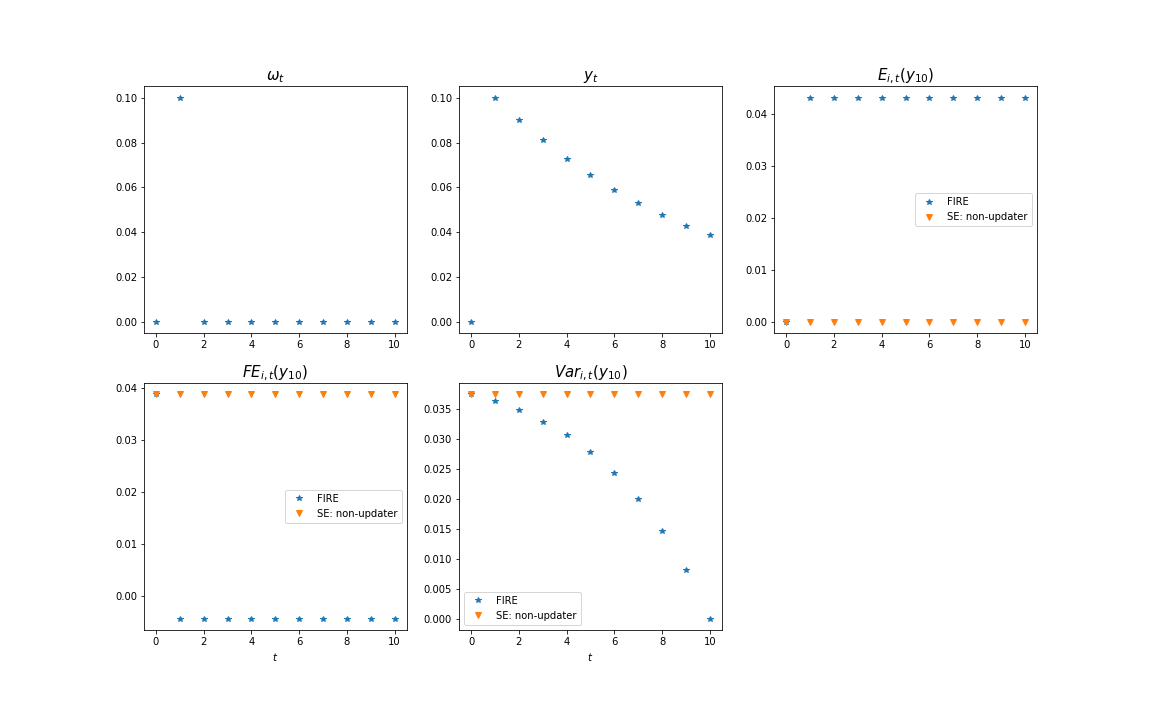
\includegraphics[scale=0.25]{figuresDraft/ir_indse} 
\end{figure}
\end{frame}


\begin{frame}{Impulse responses to shocks: population moments}

$$\textrm{True Process} \quad  \rho=0.9, \quad \sigma_\omega=0.1, \quad \omega_1 = 0.1$$
$$\textrm{SE} \quad \quad  \lambda = 0.4 $$ 

\begin{figure}
	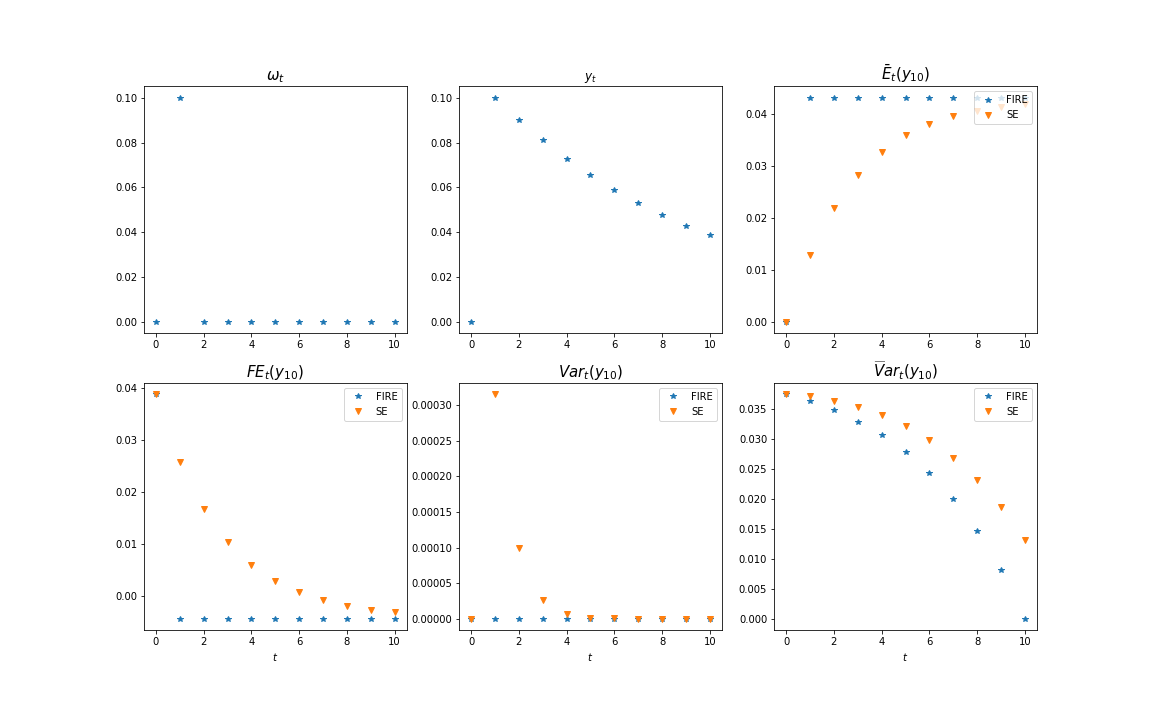
\includegraphics[scale=0.25]{figuresDraft/ir_popse} 
\end{figure}

\end{frame}

\subsection{Noisy Information(NI)}

\begin{frame}{Noisy Information: assumptions}
\begin{itemize}
	\item Individual only observes noisy signals 
	\begin{eqnarray*}
		\begin{aligned}
			& s_{i,t}=[s^{pb}_t, s^{pr}_{i,t}]' \in I_{i,t} \\
			&\text{public signal:} \quad s^{pb}_t = y_t + \epsilon_t, \quad \epsilon_t \sim N(0,\sigma^2_\epsilon)\\ 
			& \text{private signal:} \quad s^{pr}_{i,t} = y_t + \xi_{i,t} \quad \xi_{i,t} \sim N(0,\sigma^2_\xi)
		\end{aligned}
	\end{eqnarray*} 
   
	\item Kalman filtering (simply normal updating if $\rho$=0)
\end{itemize}
\end{frame}



\begin{frame}{Impulse responses to shocks: individual moments}


$$\textrm{True Process} \quad   \rho=0.9, \quad \sigma_\omega= 0.1, \quad \omega_1 = 0.1$$
$$ \textrm{SE:} \quad  \lambda = 0.5; \quad \textrm{NI:} \quad \sigma_\xi = 0.1, \quad \sigma_\epsilon = 0.1$$

\begin{figure}
	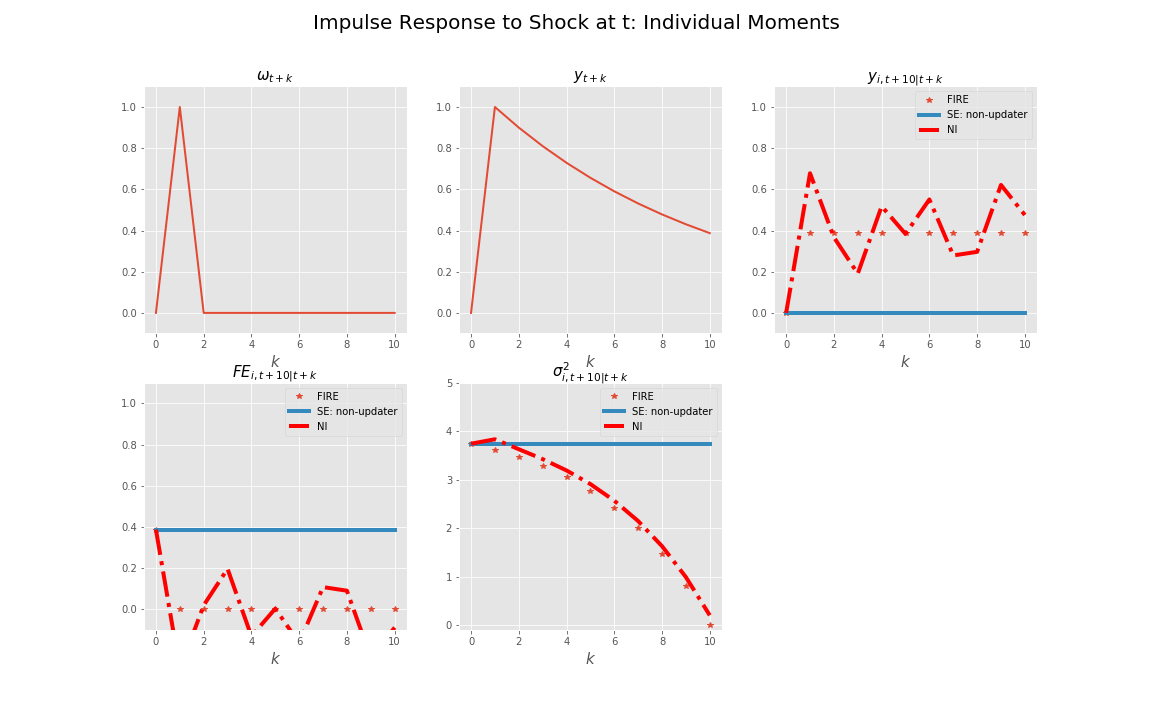
\includegraphics[height=6.3cm,width=10cm]{figuresDraft/ir_indseni} 
\end{figure}

\end{frame}

\begin{frame}{Impulse responses to shocks: population moments}


$$\textrm{True Process} \quad   \rho=0.9, \quad \sigma_\omega= 0.1, \quad \omega_1 = 0.1$$
$$ \textrm{SE:} \quad  \lambda = 0.5; \quad \textrm{NI:} \quad \sigma_\xi = 0.1, \quad \sigma_\epsilon = 0.1$$

\begin{figure}
	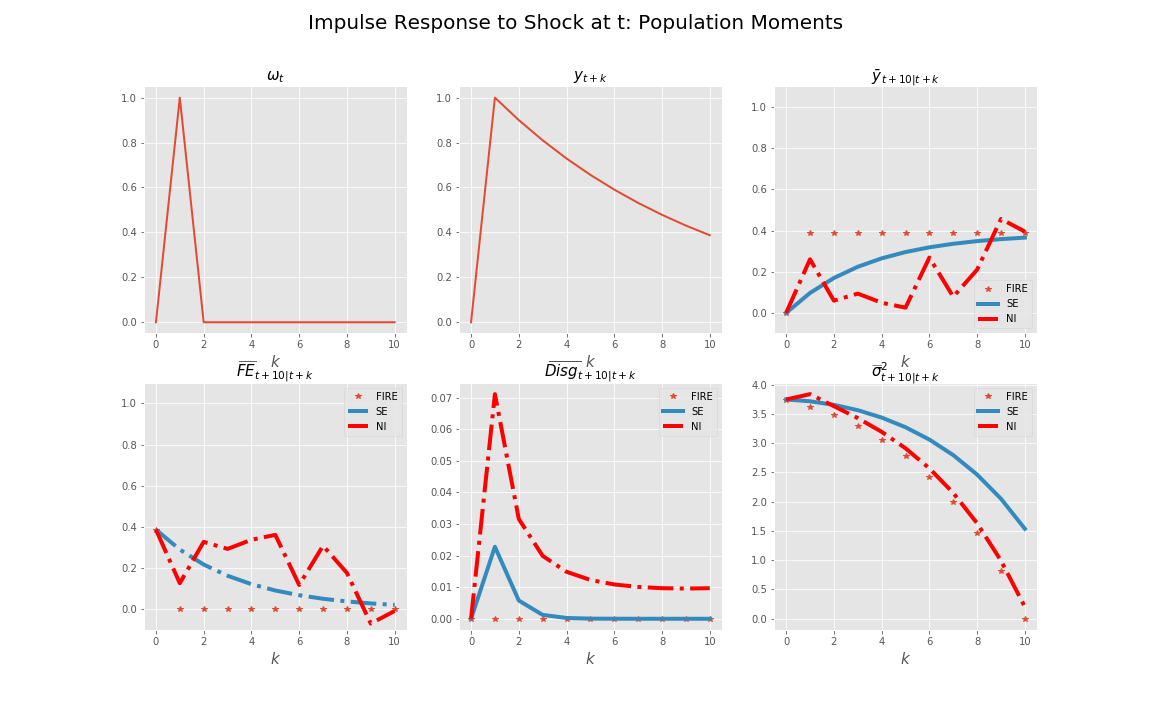
\includegraphics[height=6.3cm,width=10cm]{figuresDraft/ir_popseni} 
\end{figure}

\end{frame}

%\begin{frame}{Noisy Information: predictions}
%\begin{itemize}
%	\item \textbf{Similar to Sticky Expectation}
%	\begin{enumerate}
%\item \textbf{Macro rigidity}: population forecasts partially respond to shocks
% \item \textbf{Non-response of variance}: both individual and population variance \textcolor{blue}{does not respond to} shocks.   
% \end{enumerate}
%\item \textbf{Different from Sticky Expectation}

%	\begin{enumerate}
%	\item \textbf{Micro rigidity}: both individual and population forecast \textcolor{blue}{partially} respond to shocks 
%	\item \textbf{Horizon-sensitive rigidity}: rigidity decreases with horizon
%	\item \textbf{Increasing disagreements:} population disagreements \textcolor{blue}{increase} over time as approaching $t+h$
%	\item \textbf{Shock-specific responses:} different impacts of fundamental shocks, or simply news shocks 
%\end{enumerate}
%\end{itemize}

%\end{frame}


\begin{frame}{A detailed look into noisy information}


\begin{figure}
	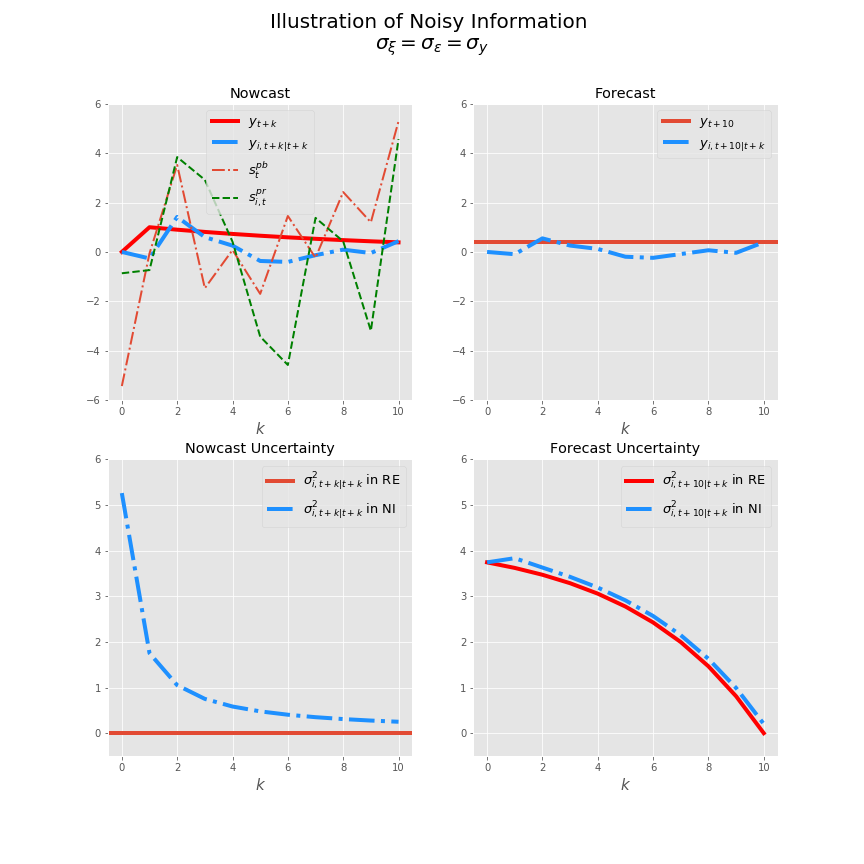
\includegraphics[height=8cm,width=8cm]{figuresDraft/ni_illustration} 
\end{figure}

\end{frame}


\begin{frame}{Implied rigidity of different models}


\begin{figure}
	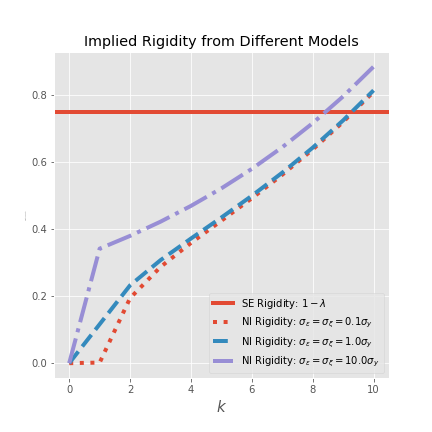
\includegraphics[height=5cm,width=8cm]{figuresDraft/rigidity} 
\end{figure}

\end{frame}



\begin{frame}{Other theories on to-do-list}
\begin{itemize}
	\item \textbf{Rational Inattention:} attentiveness endogenously respond to variances
	\item \textbf{Learning}: the structural parameter $\rho$ is not known, thus the agent learns about it as if an econometrician does
\end{itemize}
\end{frame}

\begin{frame}{Identification strategies 1: testing rigidity models}

\begin{itemize}
	\item\cite{coibion2012can}
	\begin{itemize}
		\item \textcolor{blue}{FEs} respond to shocks and serially correlated. 
	\end{itemize}
	\item \textbf{Additional in this paper}
	\begin{itemize}
		\item \textcolor{blue}{Uncertainty} does not depend on shocks; and serially correlated. 
	\end{itemize}
\end{itemize}

\end{frame}

\begin{frame}{Identification strategies 2: differentiating theories}
\begin{itemize}
	\item\cite{coibion2012can}
	\begin{itemize}
		\item \textcolor{blue}{FEs} do not depend on past realizations according to baseline SE and NI; but do so according to heterogeneous priors or precision models. 
		\item Implied rigidity does not differ across shocks according to SE but differs according to NI. 
		\item \textcolor{blue}{Disagreements} rise after shocks according to baseline SE, strategic interactions and heterogeneous priors but invariant according to baseline NI.
	\end{itemize}
	\item \textbf{Additional in this paper}
	\begin{itemize}
		\item \textcolor{blue}{Uncertainty} do not depend on shocks per se according to baseline SE and NI, instead on degree of information rigidity.
	\end{itemize}
\end{itemize}

\end{frame}

\section{Data and Methodology}


\begin{frame}{Data}
\begin{table}[]
\resizebox{\textwidth}{!}{	\begin{tabular}{lll}
		
		\hline 
		& SCE & SPF        \\
		\hline 
		Time period                                    & 2013-present                            & 2007-present             \\
		Frequency                                      & Monthly                                 & Quarterly                \\
		Sample Size                                    & 1,300                                   & 30-50                    \\
		Aggregate Var in Density                       & \textcolor{blue}{1-yr and 3-yr inflation}          & \textcolor{blue}{1-yr and 3-yr CPI and PCE}         \\
		Pannel Structure                               & stay up to 12 months                    & average stay for 5 years \\
		Demographic Info                        & Education, Income, Age        & Industry    \\
		\hline 
	\end{tabular}}
\end{table}

\end{frame}



\section{Stylized Facts}

\begin{frame}{Uncertainty and Realized Inflation}
\begin{figure}
	\centering
\label{InfVar}
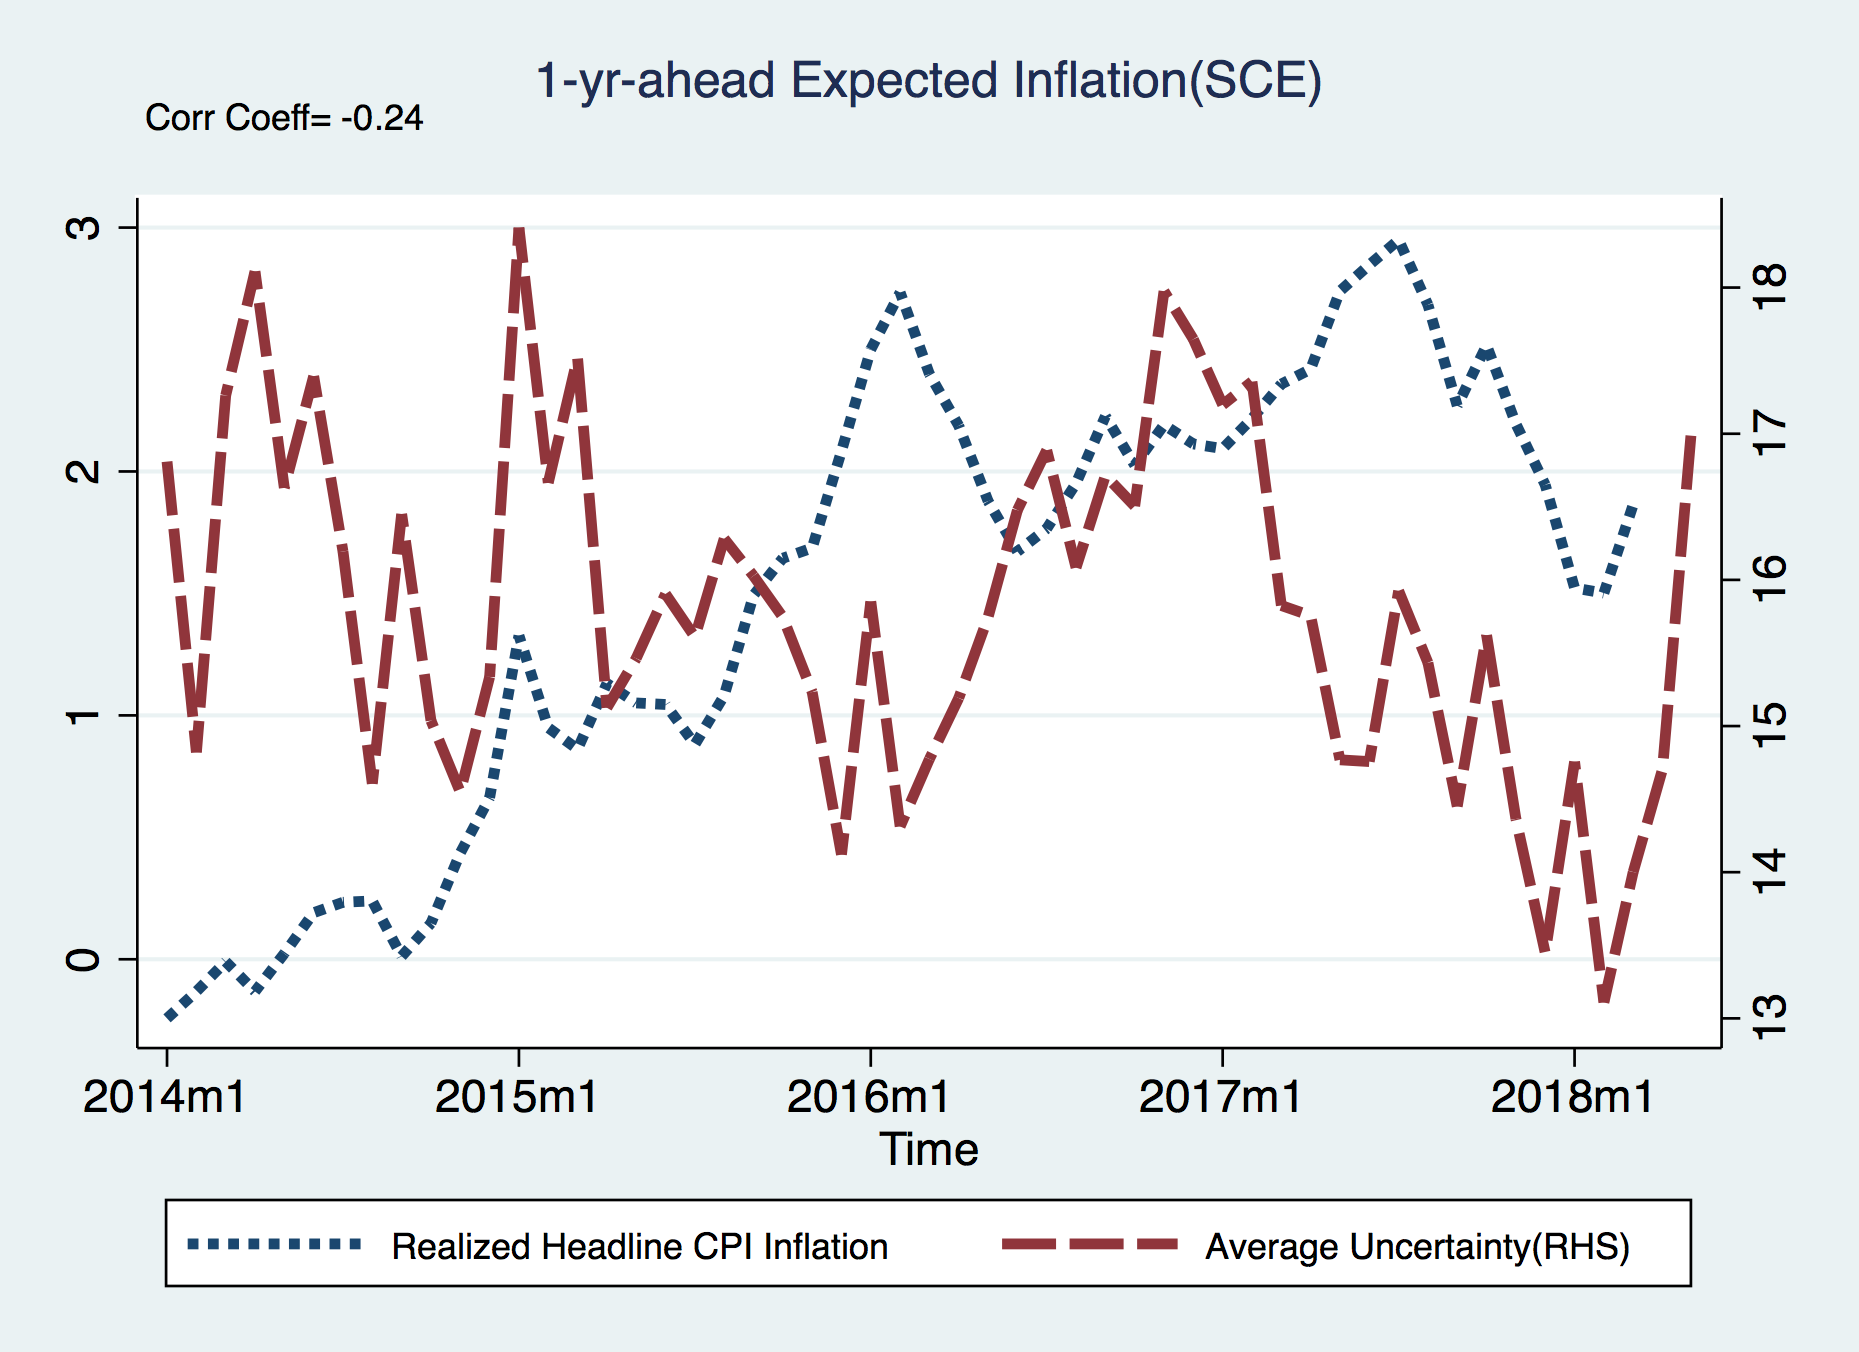
\includegraphics[width=0.33\textwidth]{figuresDraft/Inf1yf_CPIAU_varSCEM.png}
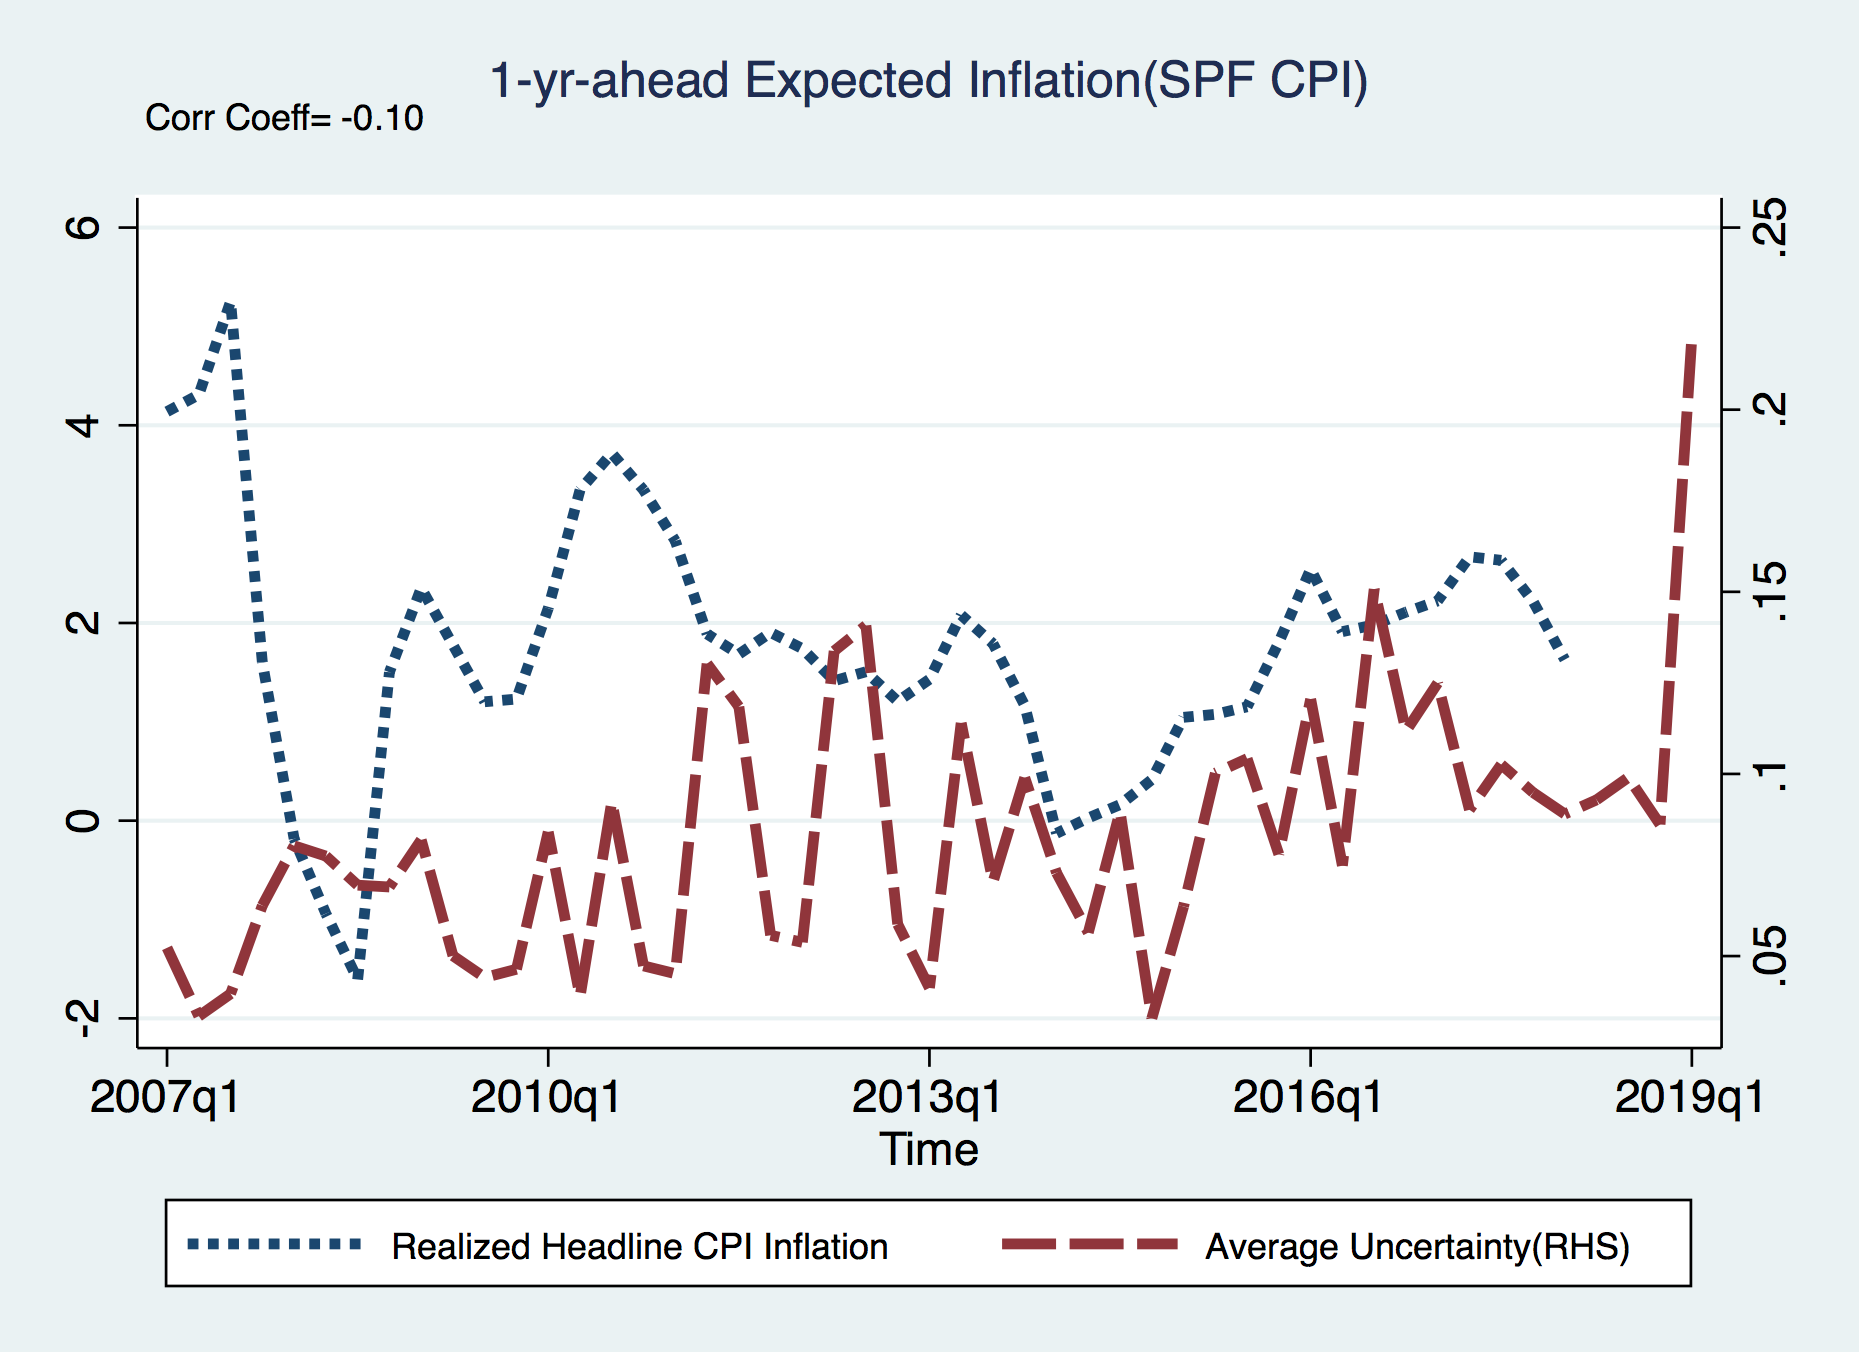
\includegraphics[width=0.33\textwidth]{figuresDraft/Inf1yf_CPIAU_varSPFCPIQ.png}
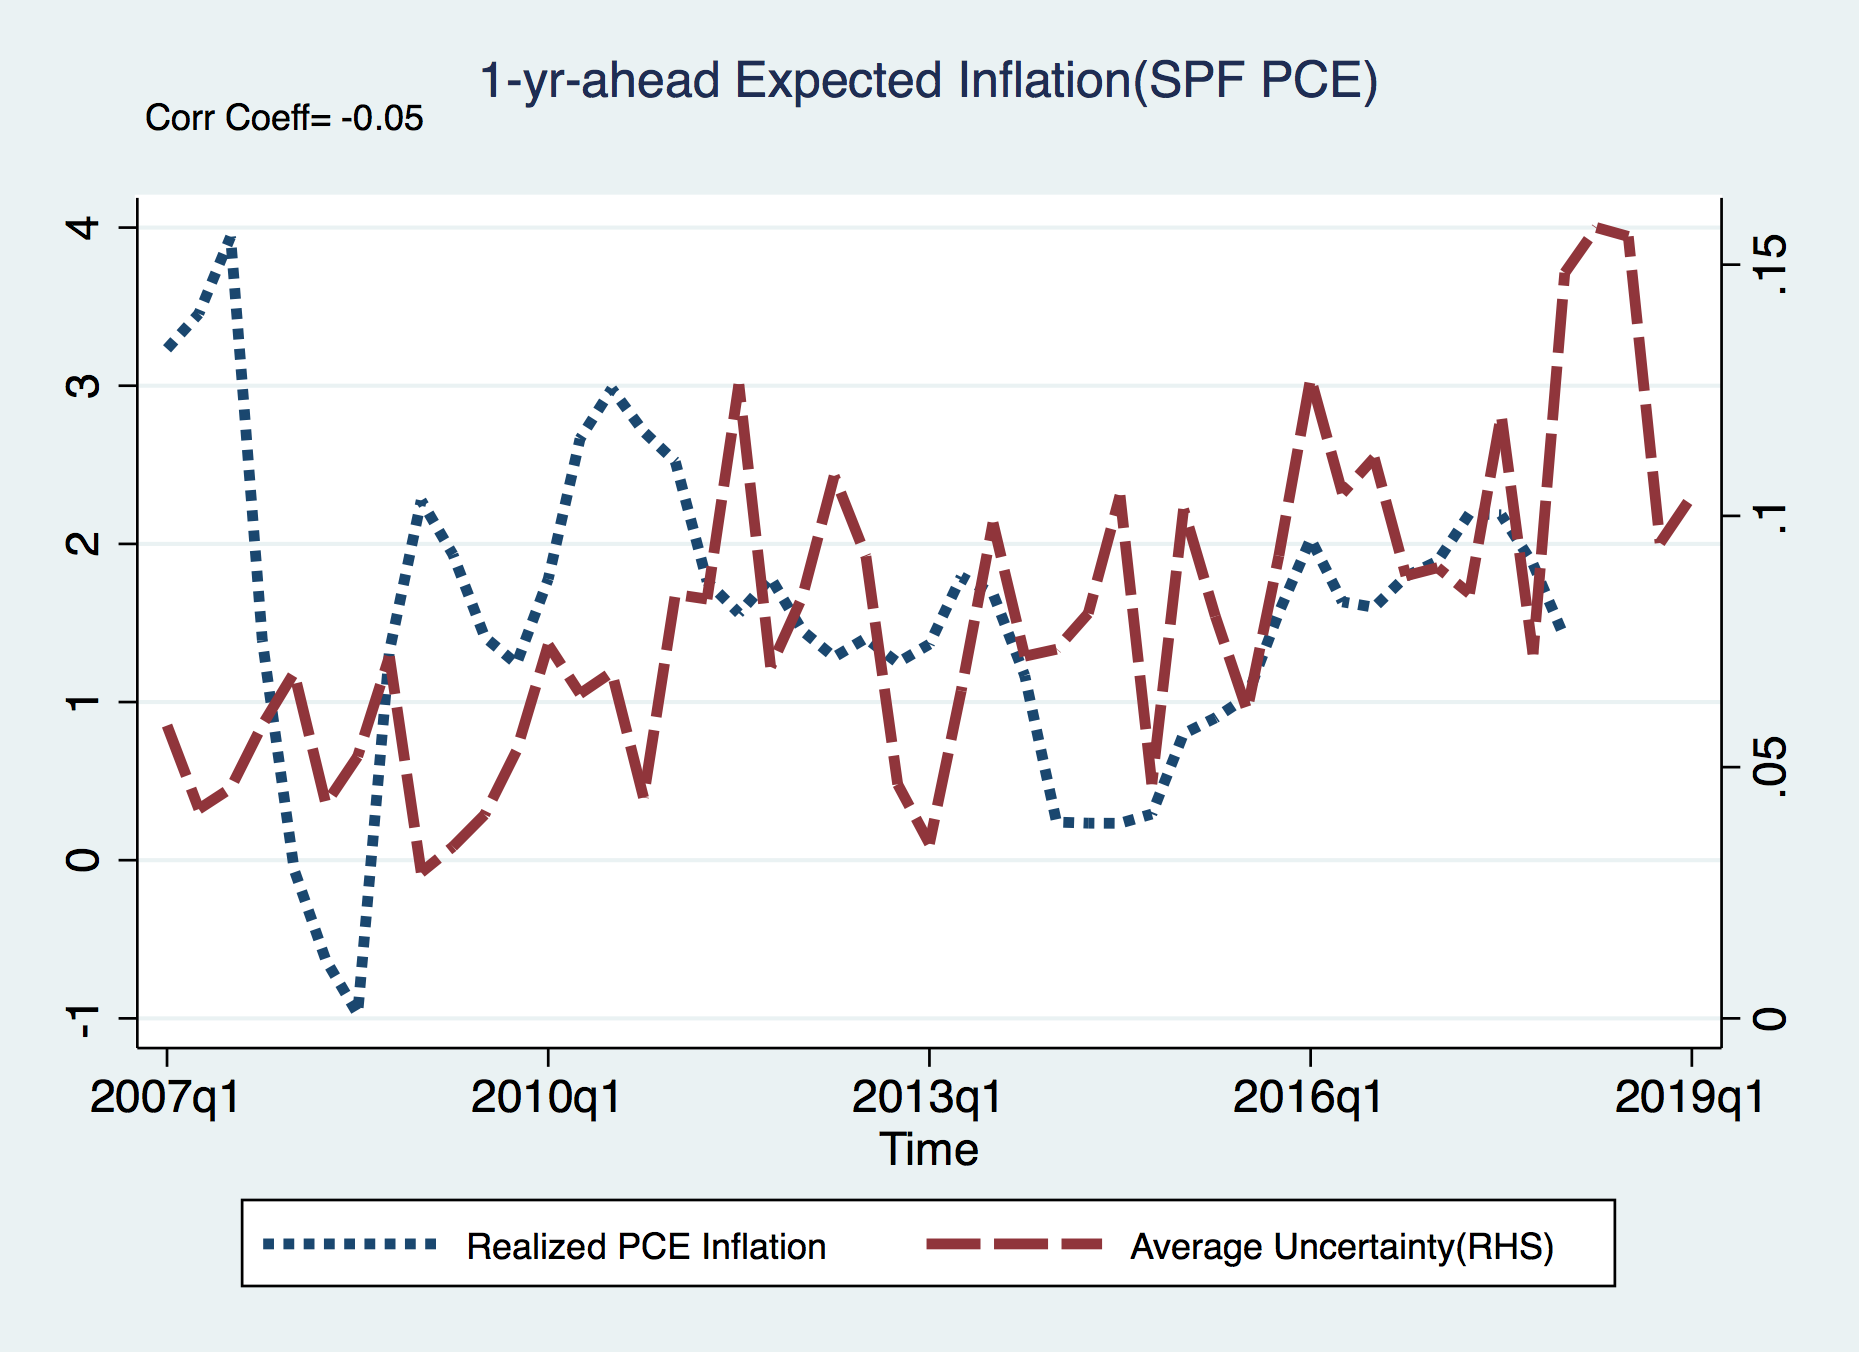
\includegraphics[width=0.33\textwidth]{figuresDraft/Inf1yf_PCE_varSPFPCEQ.png}
\end{figure}
\end{frame}

\begin{frame}{Uncertainty and Forecast Errors}
\begin{figure}
	\centering
	\label{FEVar}
	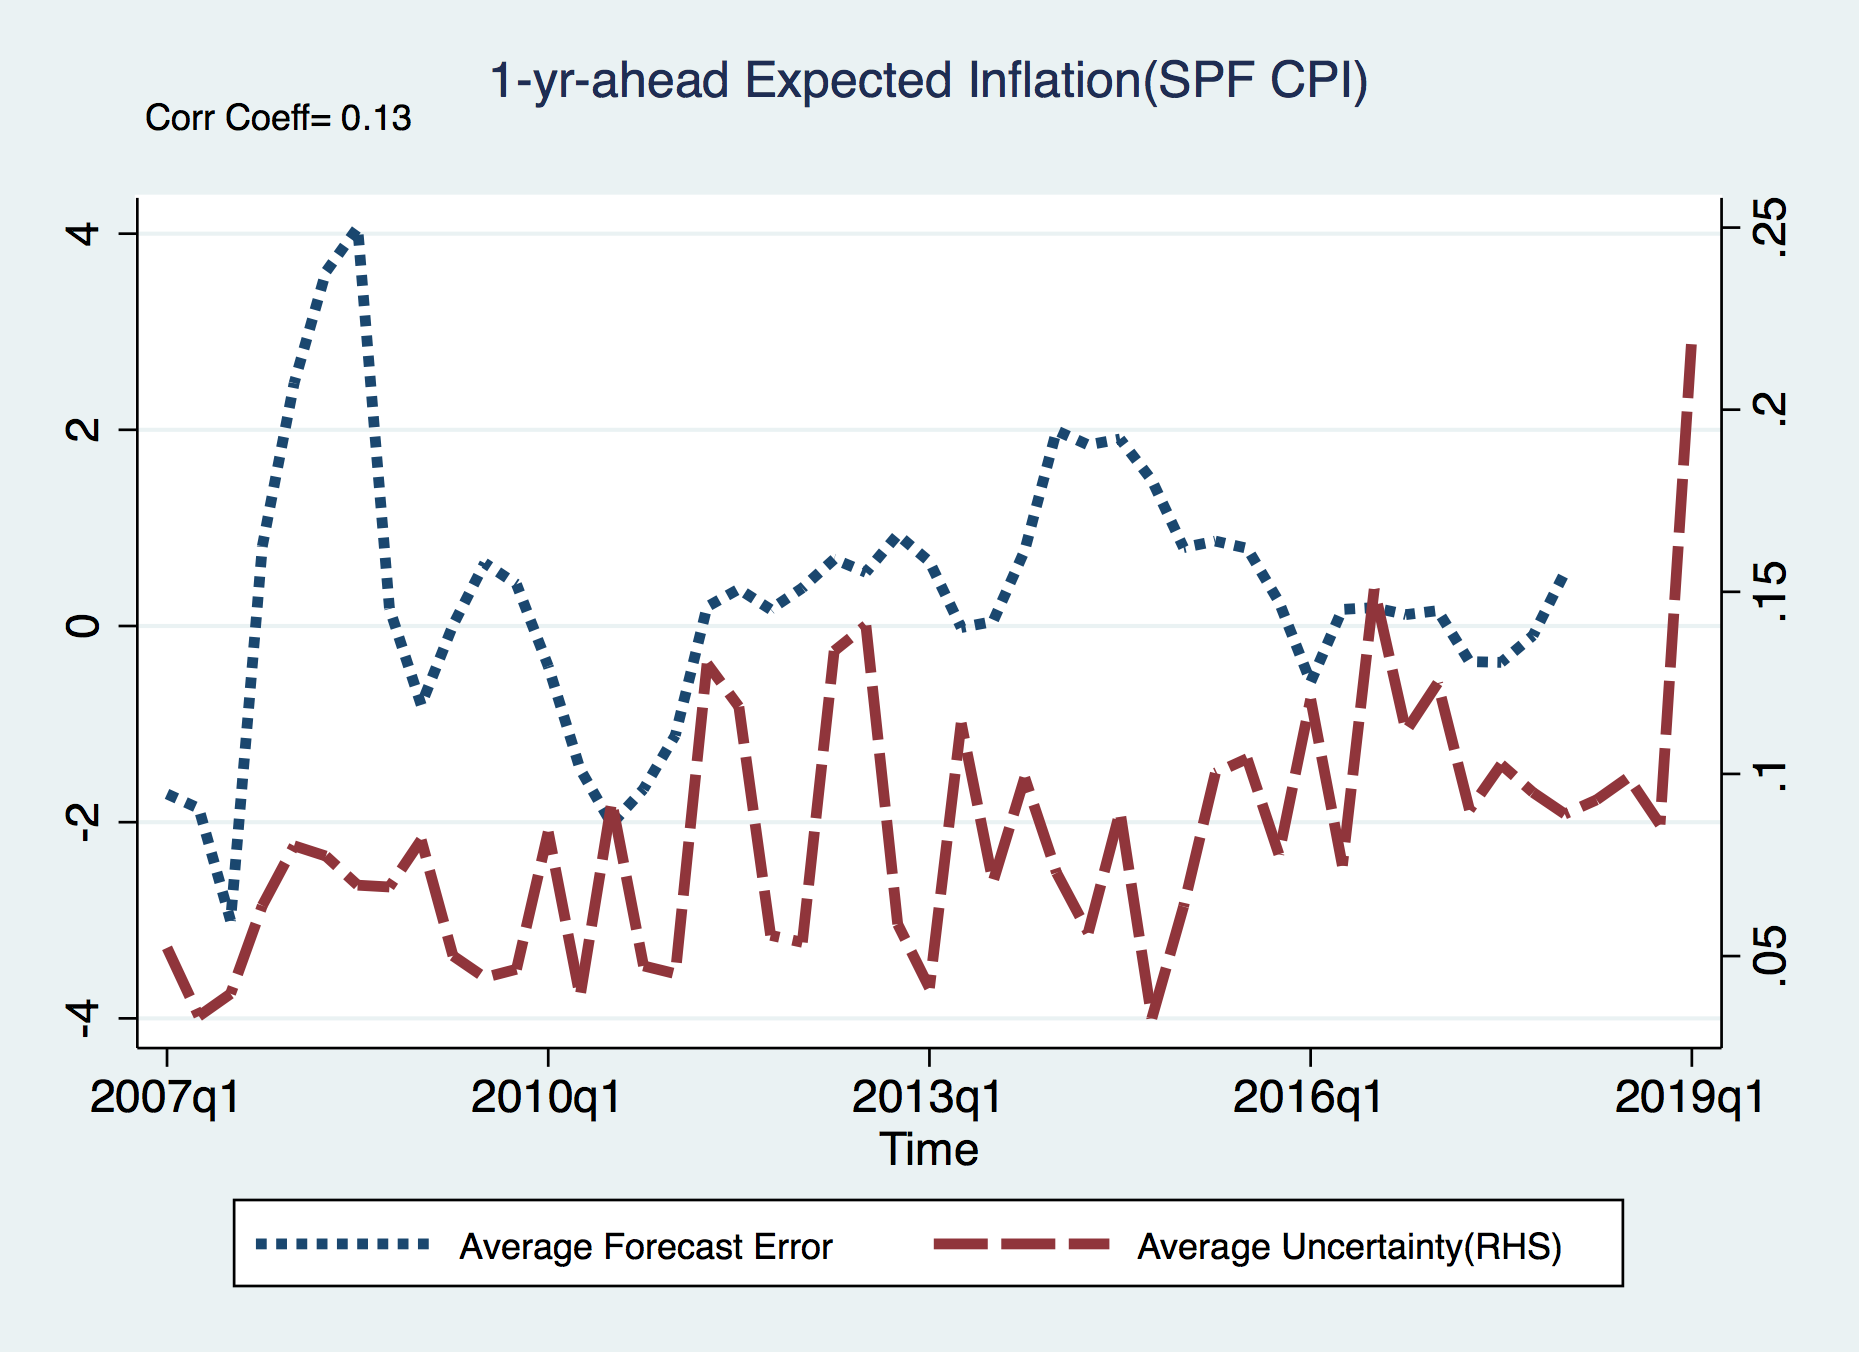
\includegraphics[width=0.33\textwidth]{figuresDraft/SPFCPI_FE_varSPFCPIQ.png}
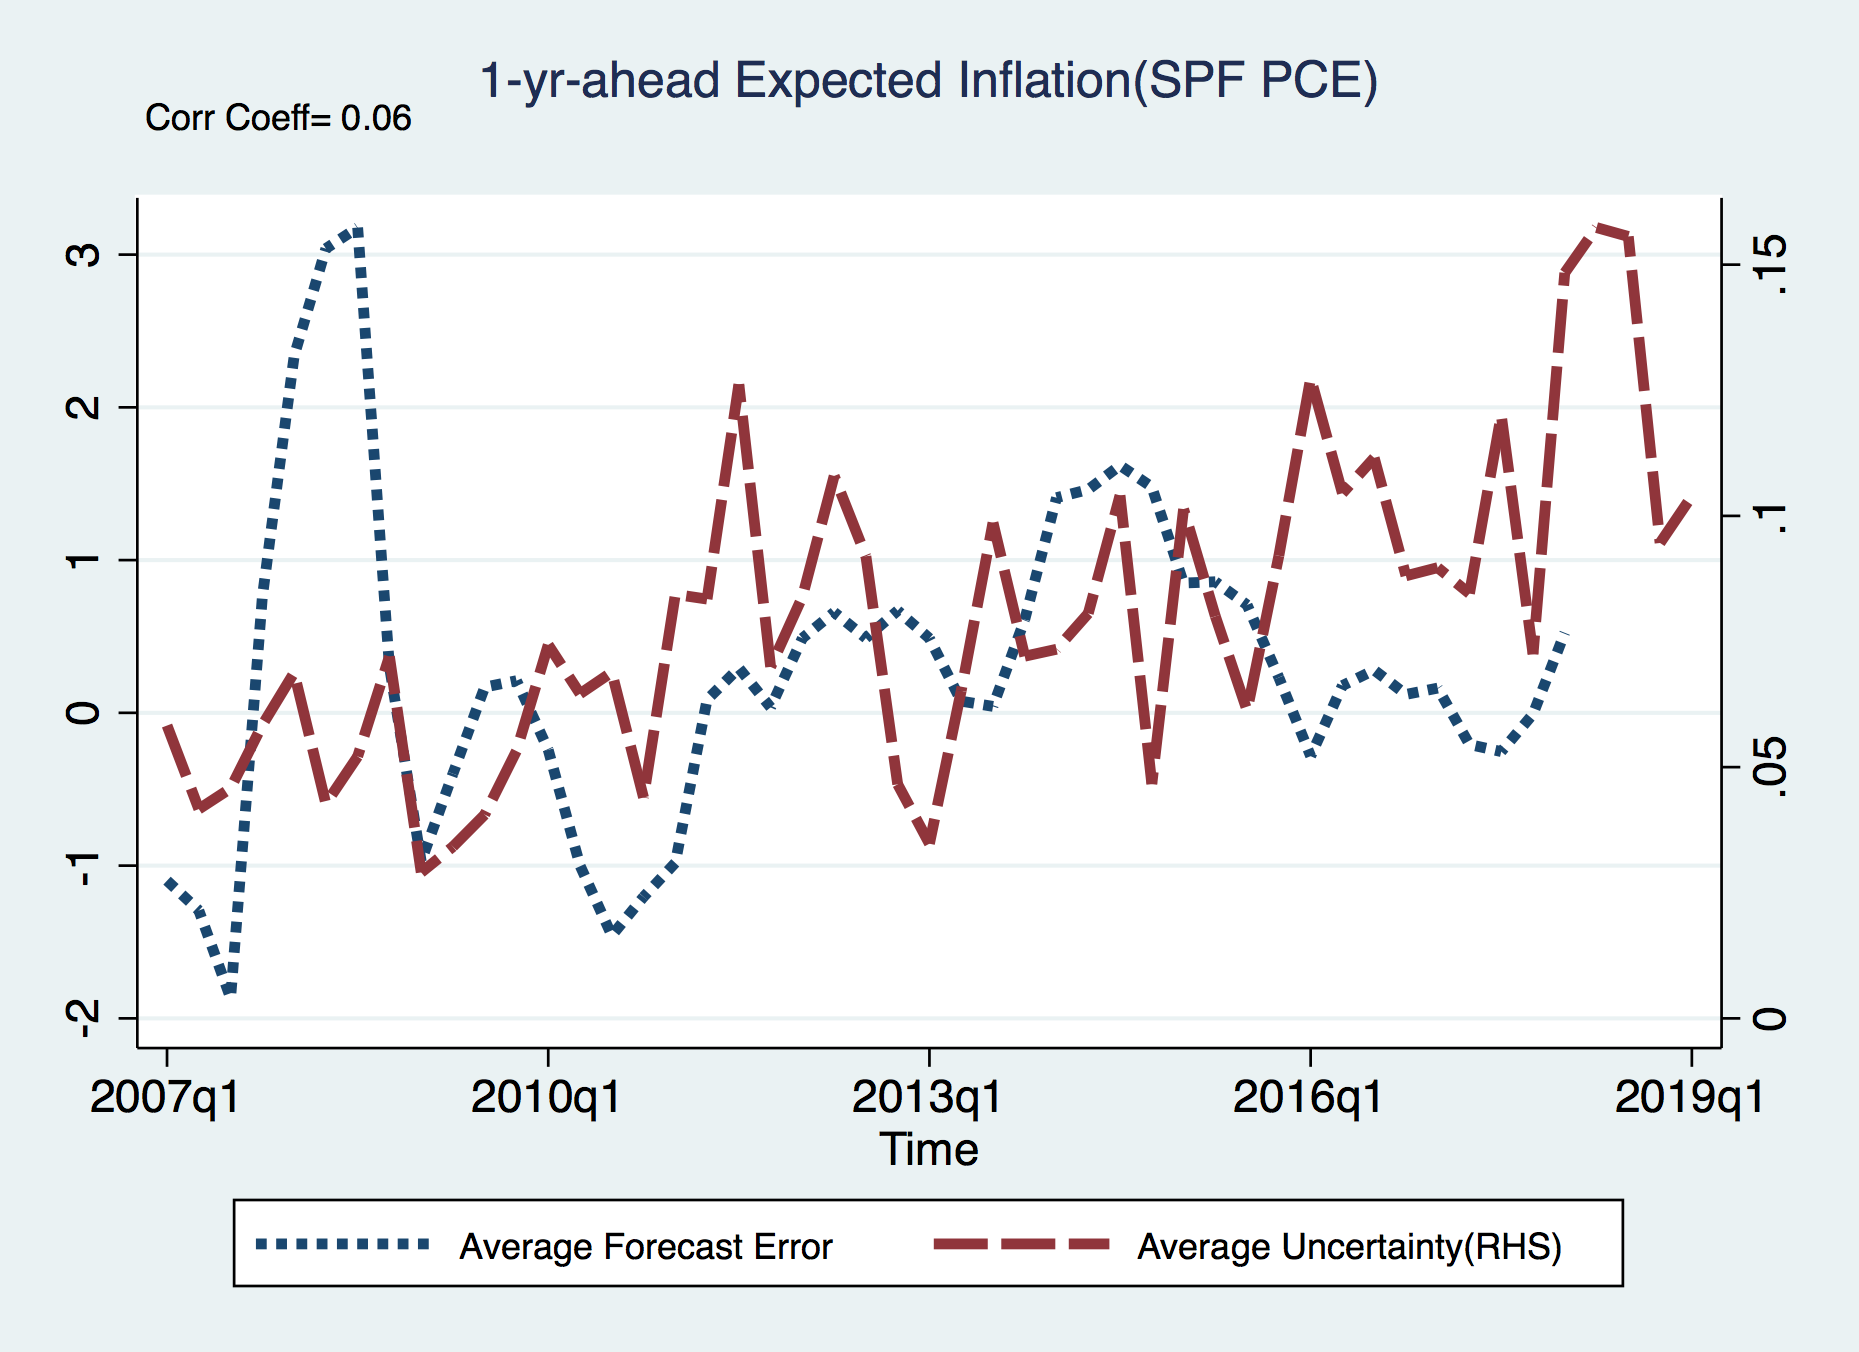
\includegraphics[width=0.33\textwidth]{figuresDraft/SPFPCE_FE_varSPFPCEQ.png}
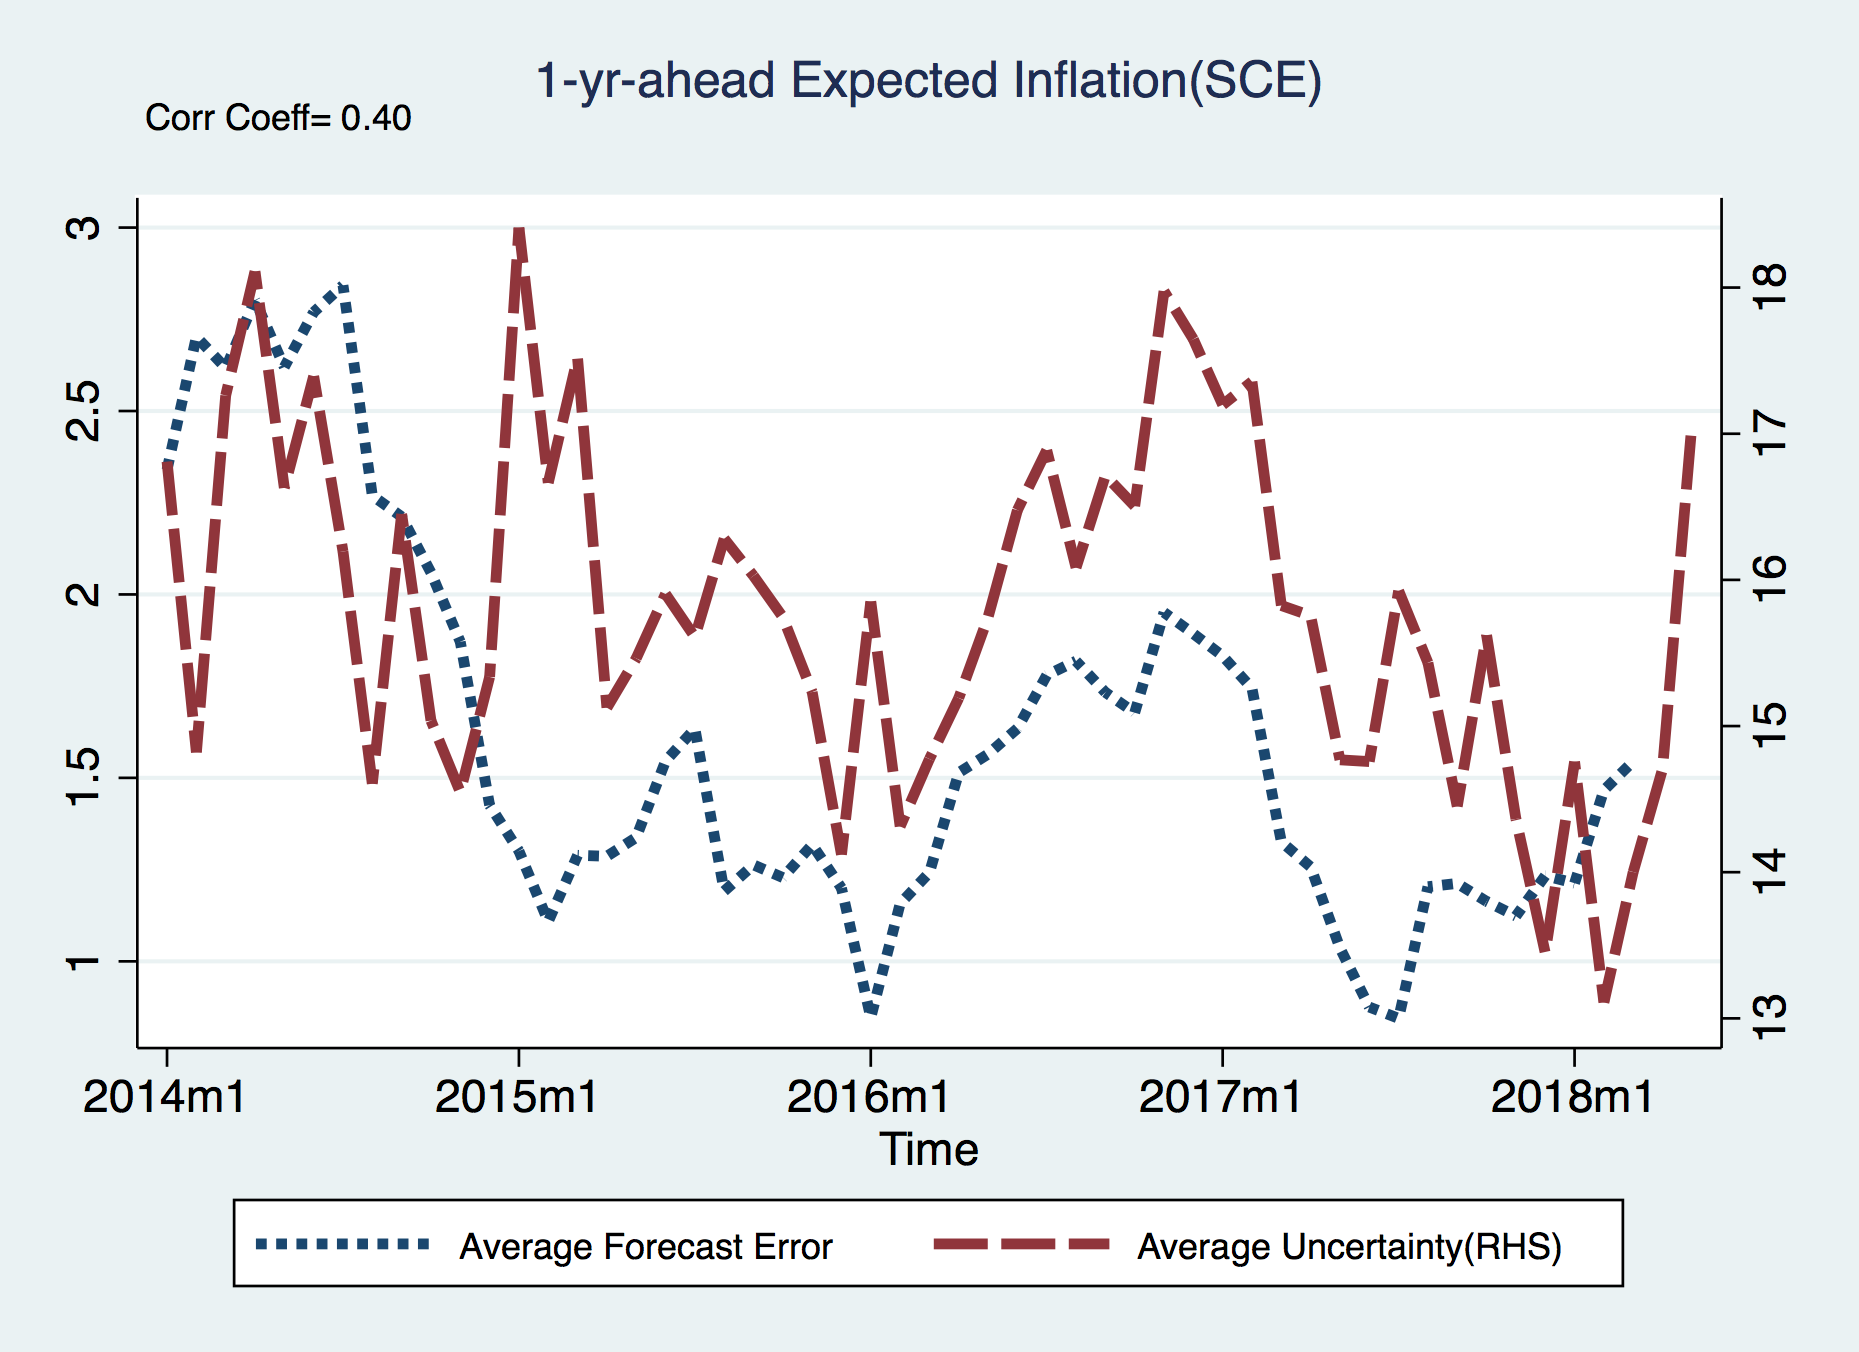
\includegraphics[width=0.33\textwidth]{figuresDraft/SCE_FE_varSCEM.png}
\end{figure}
\end{frame}


\begin{frame}{Uncertainty and Disagreements}
\begin{figure}
	\centering
\label{DisgVar}
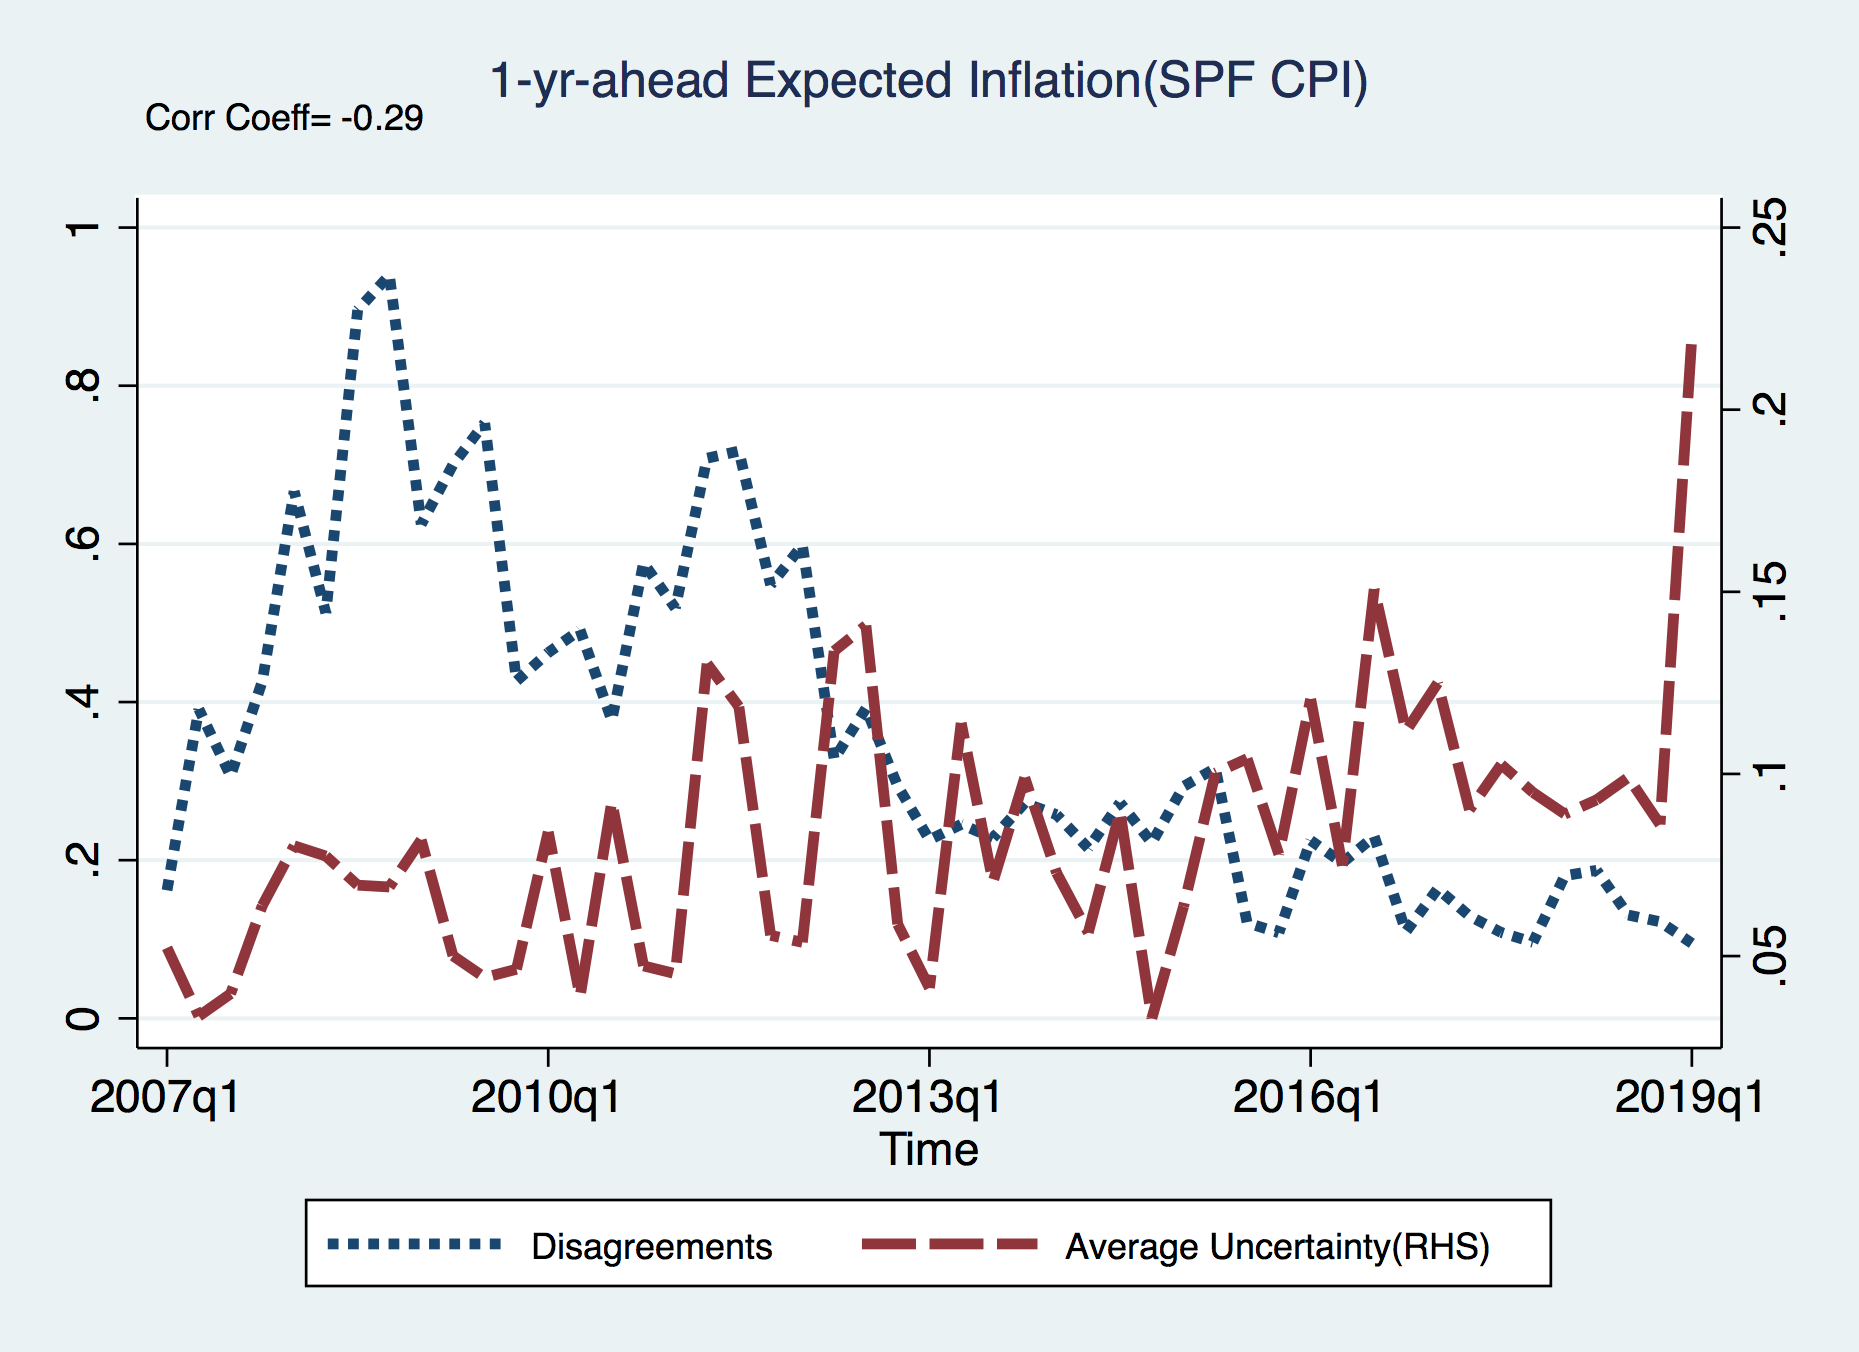
\includegraphics[width=0.33\textwidth]{figuresDraft/CPI_disg_varSPFCPIQ.png}
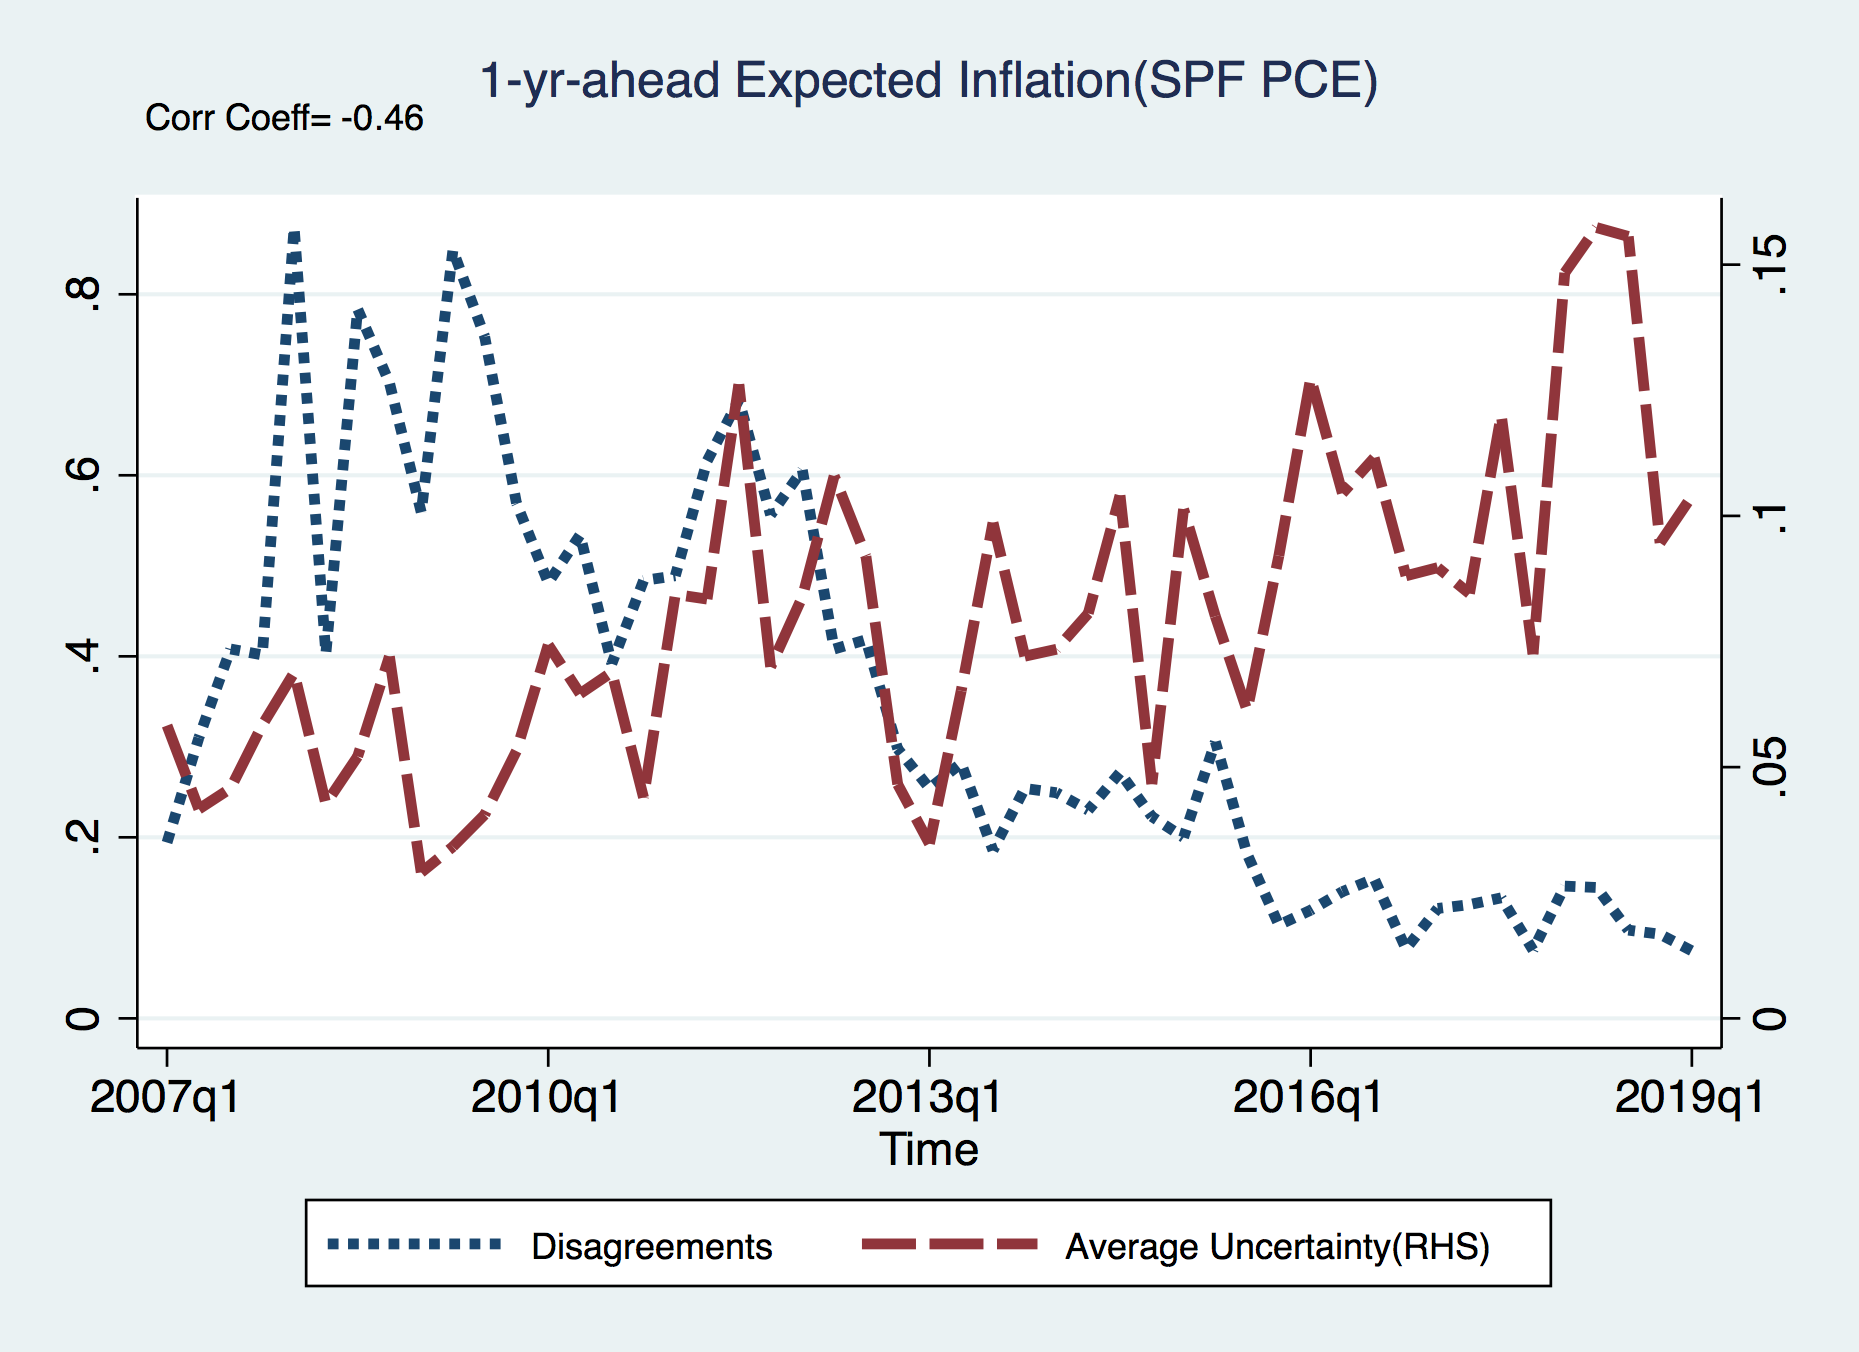
\includegraphics[width=0.33\textwidth]{figuresDraft/PCE_disg_varSPFPCEQ.png}
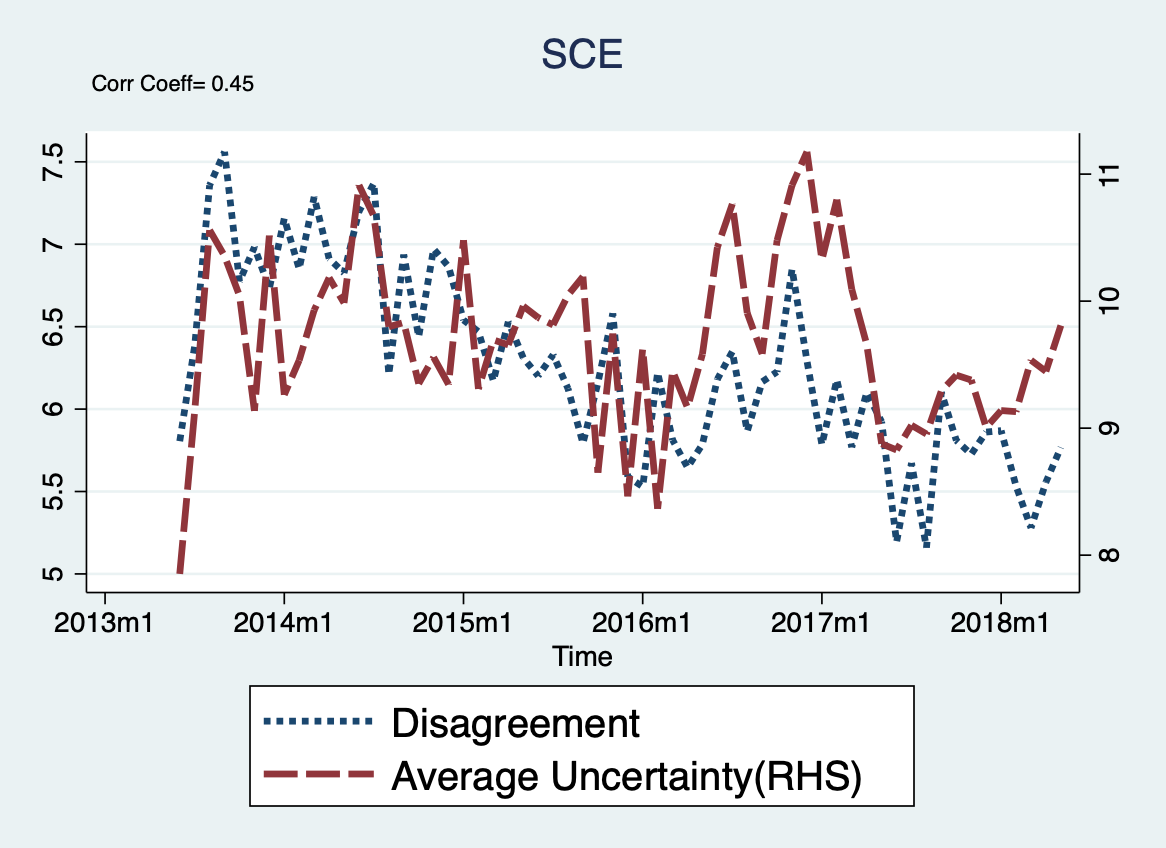
\includegraphics[width=0.33\textwidth]{figuresDraft/Q9_disg_varSCEM.png}
\end{figure}
\end{frame}



\begin{frame}{Dispersion of Mean Forecast}
\begin{figure}
	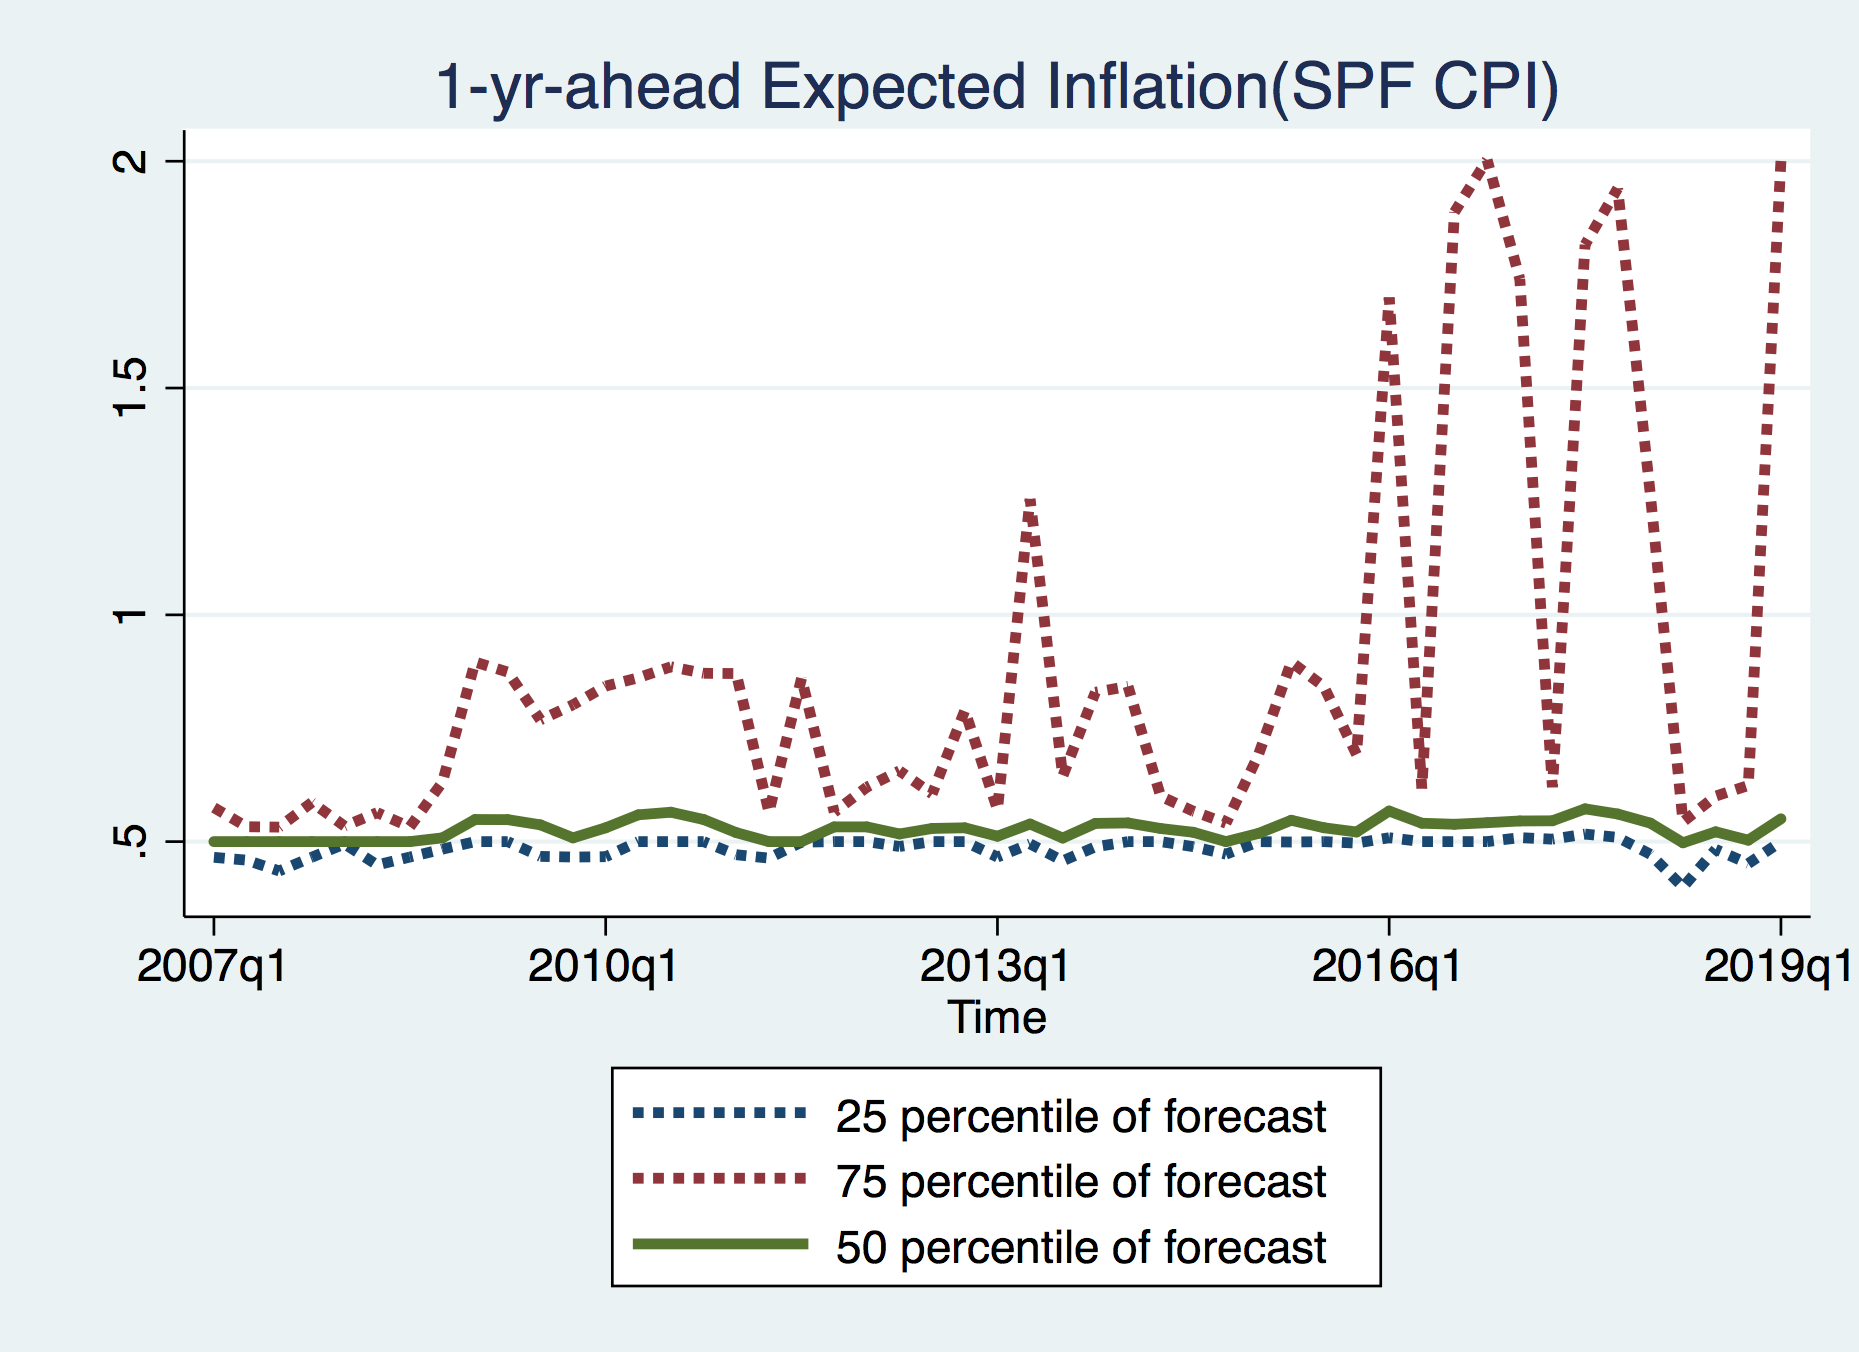
\includegraphics[width=0.33\textwidth]{figuresDraft/IQRmeanCPIQ.png} 
\smallskip
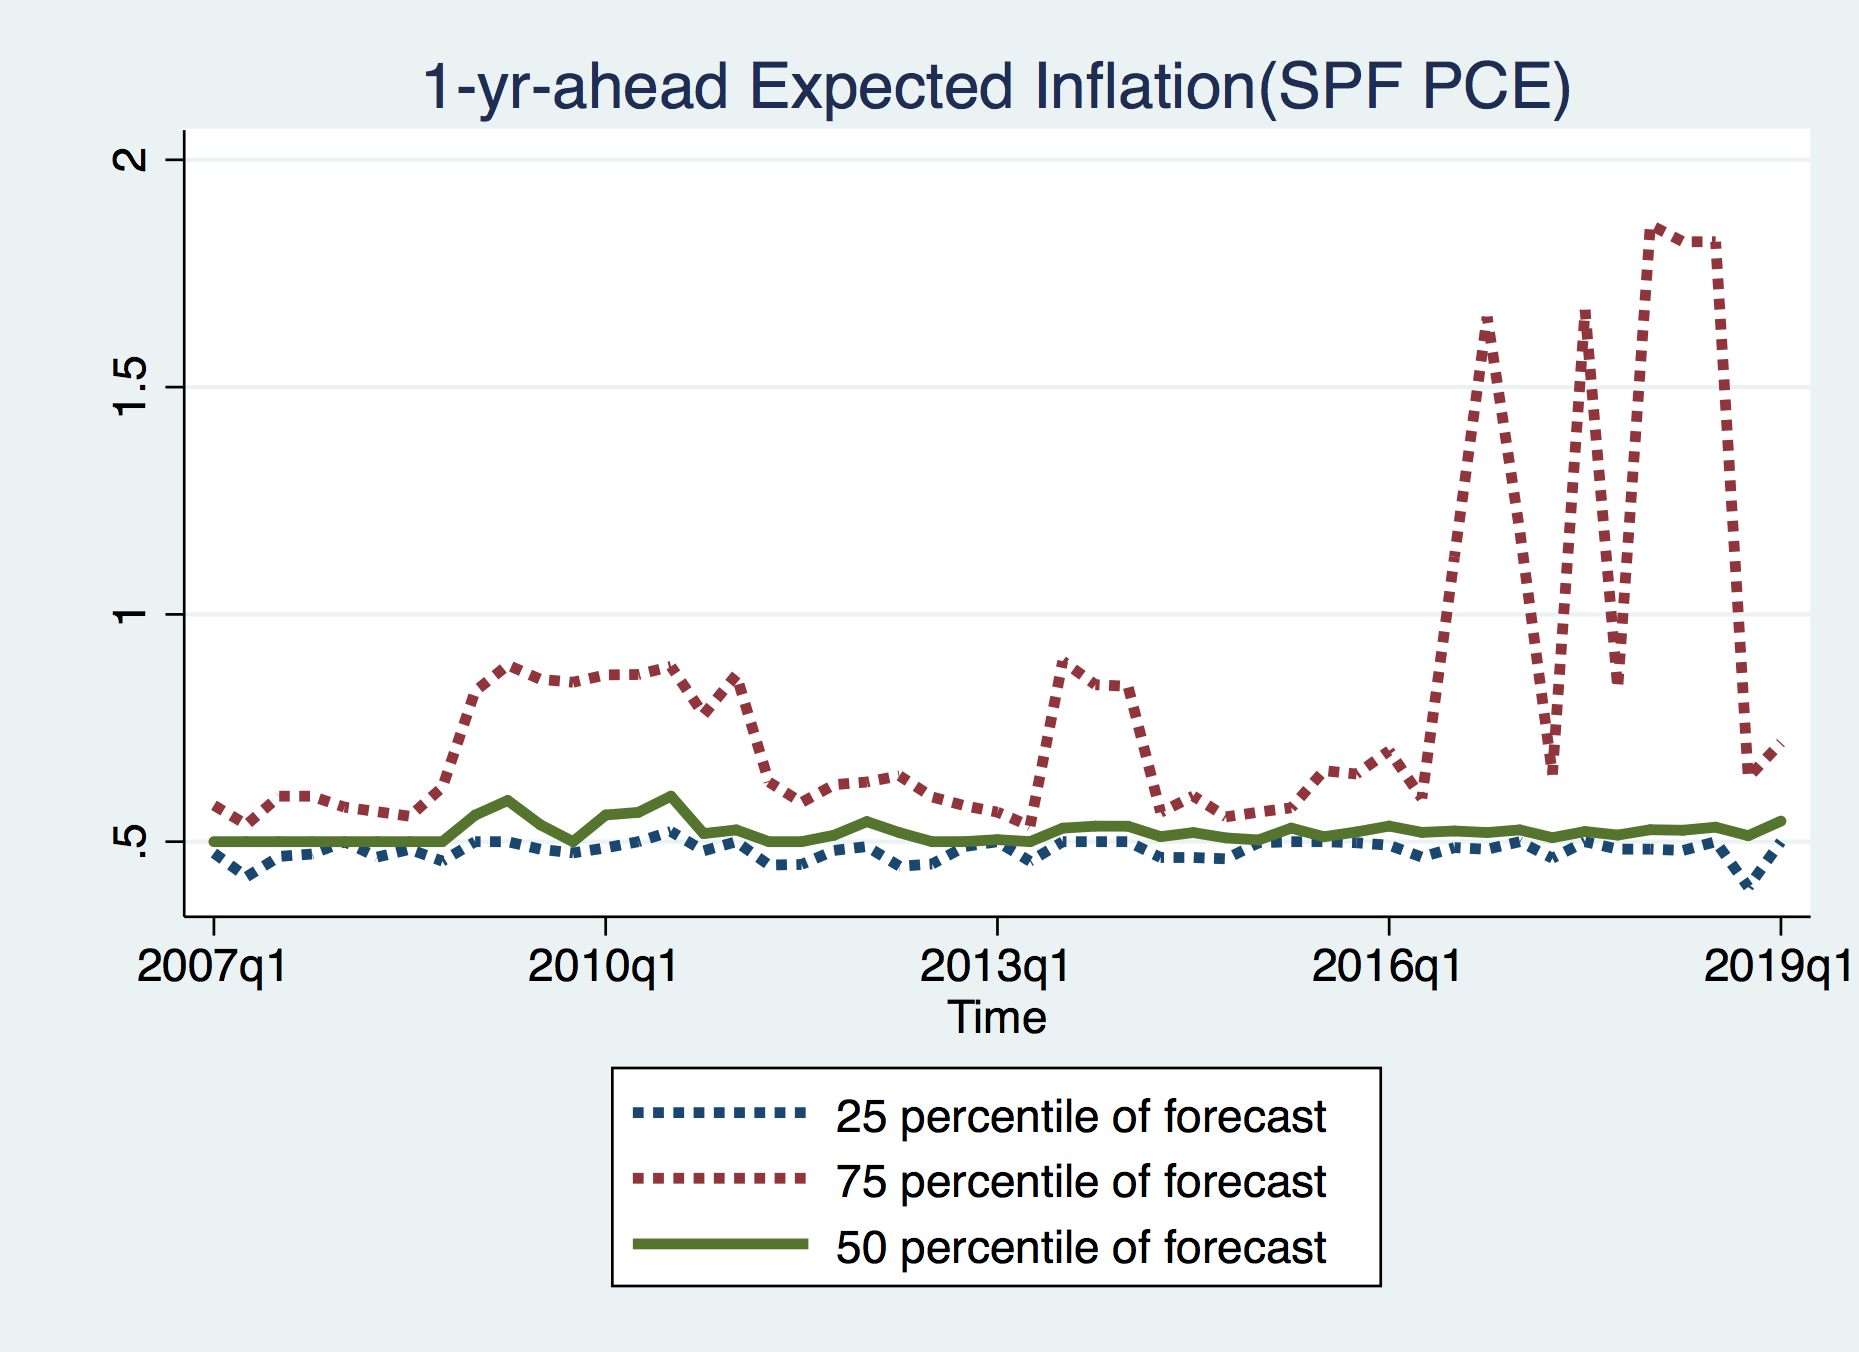
\includegraphics[width=0.33\textwidth]{figuresDraft/IQRmeanPCEQ.png}
\smallskip
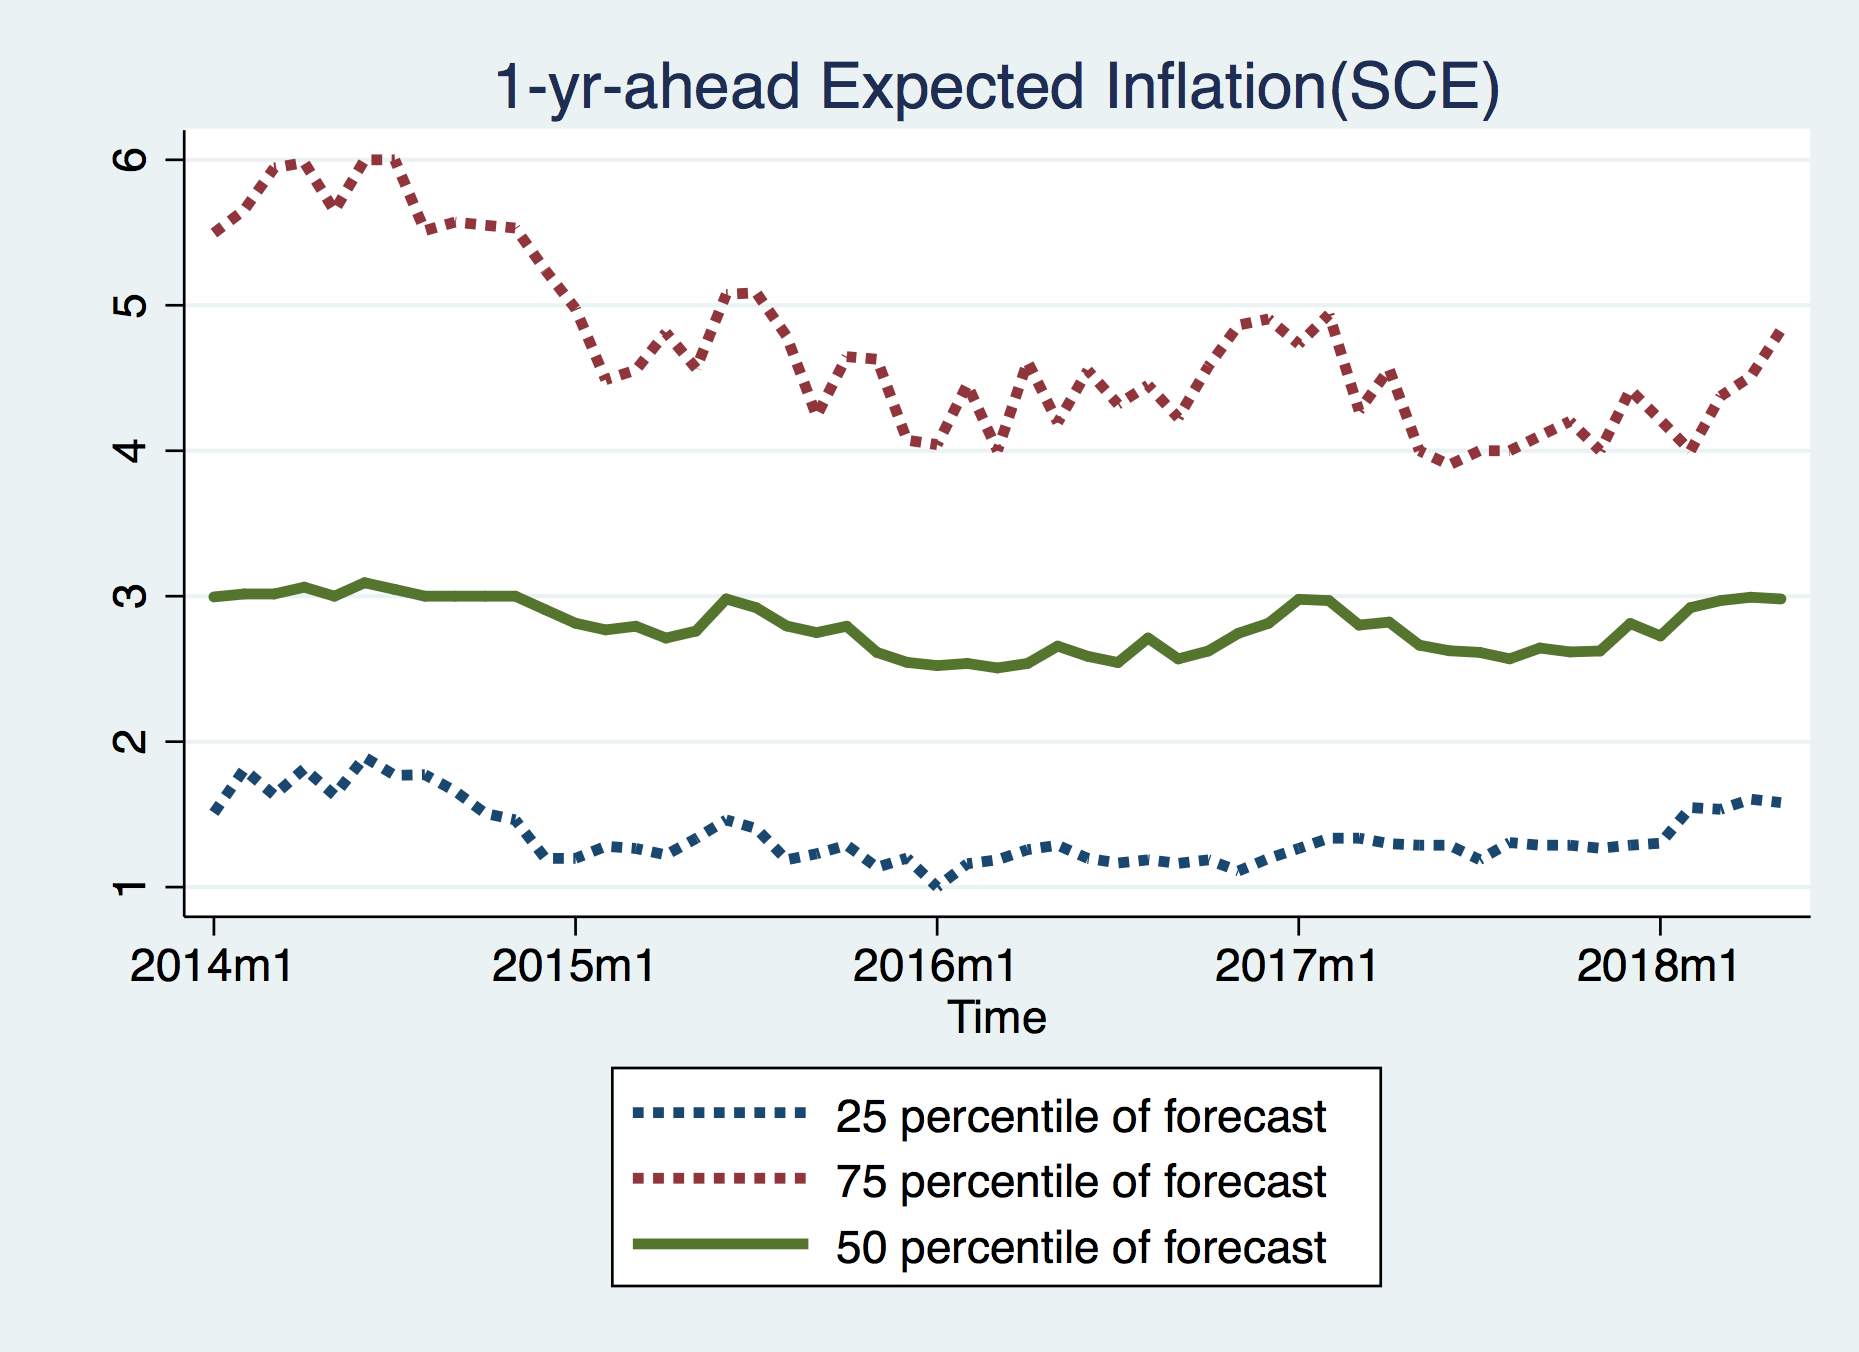
\includegraphics[width=0.33\textwidth]{figuresDraft/IQRmeanSCEM.png}
\end{figure}
\end{frame}


\begin{frame}{Dispersion of Uncertainty}
\begin{figure}
	\label{IQR_Unceratitny}
	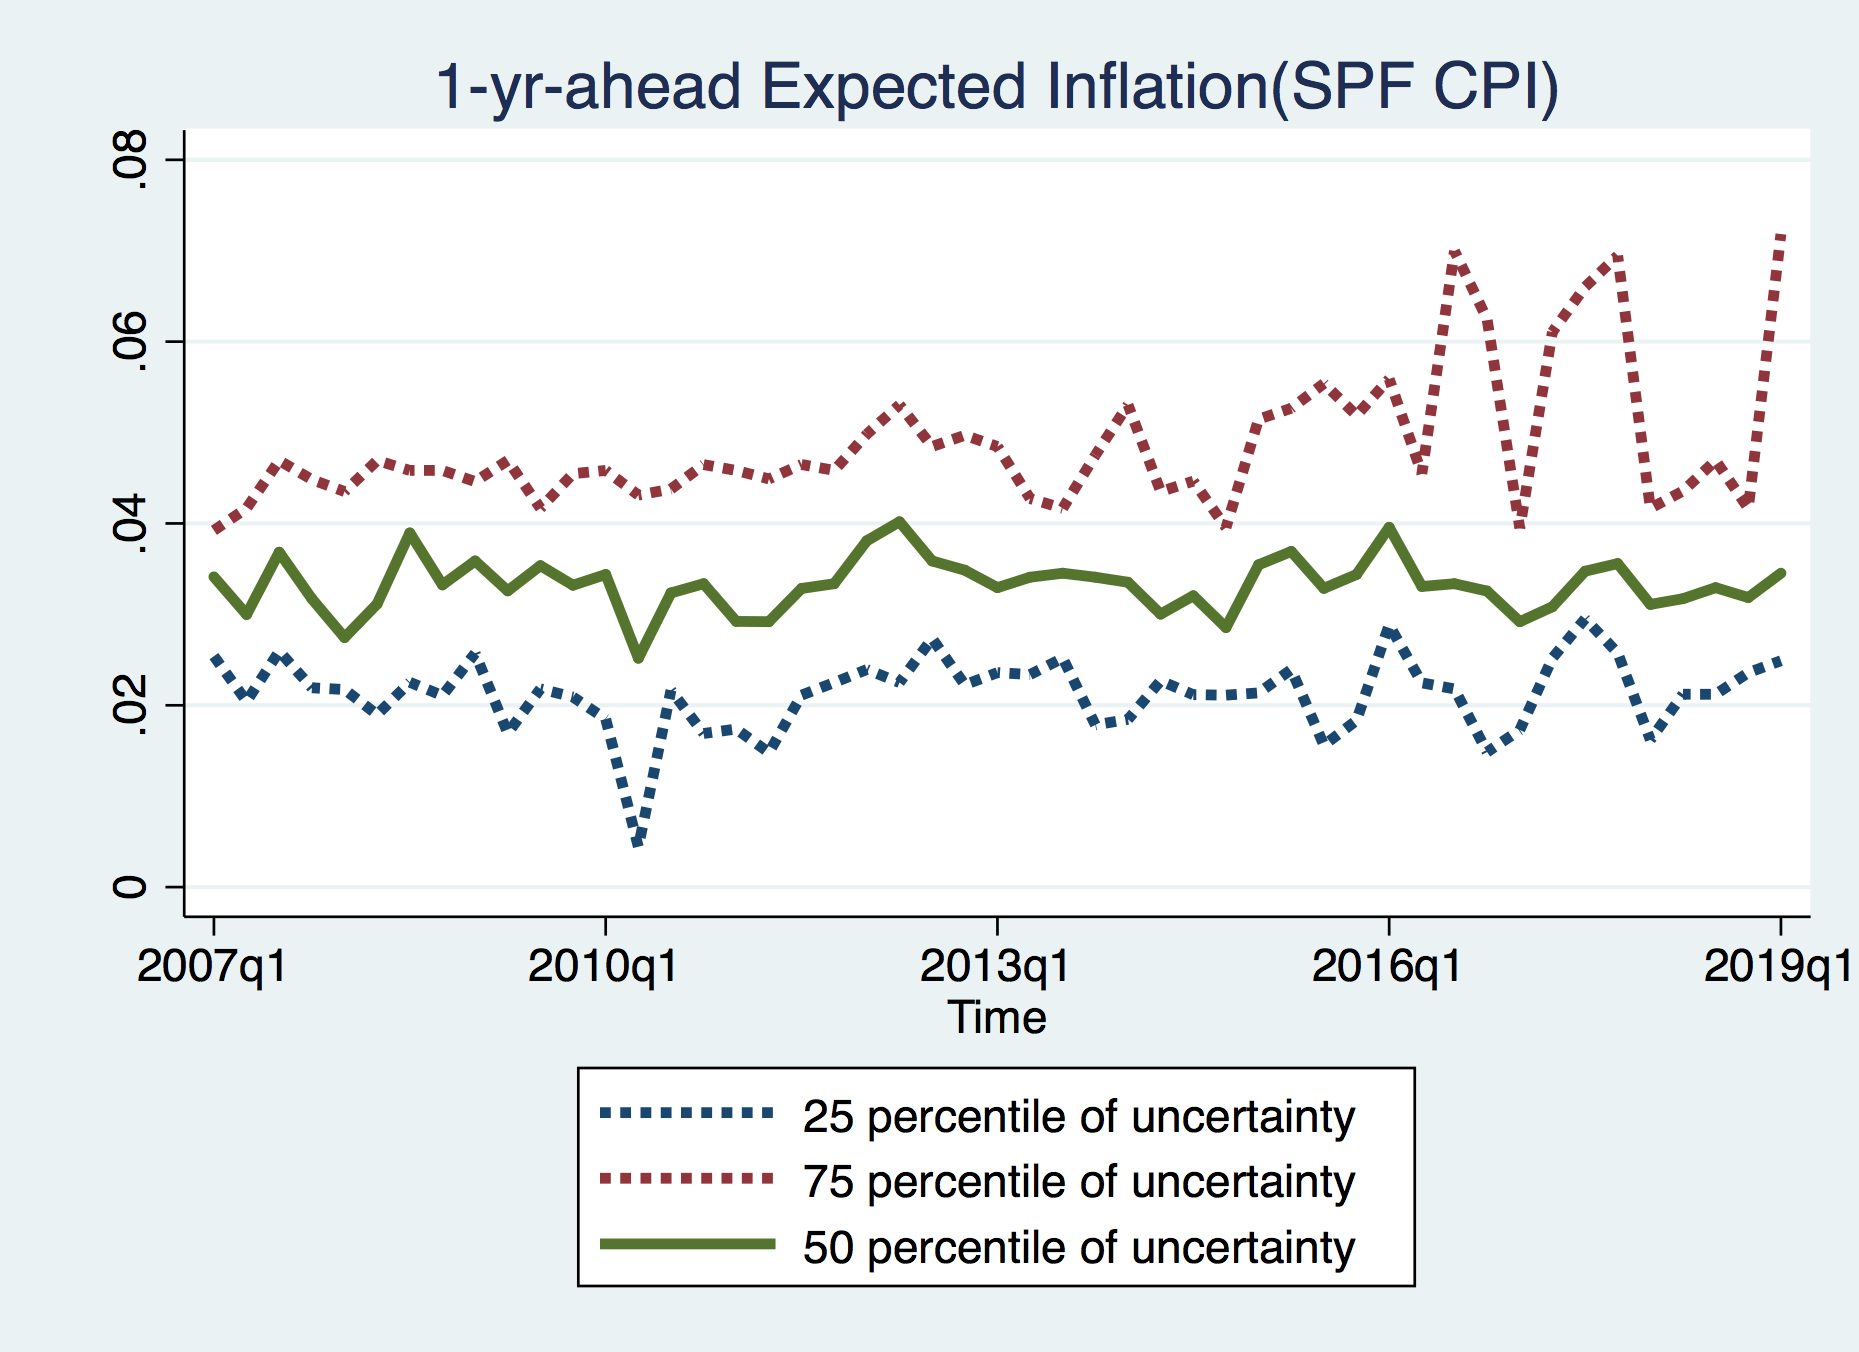
\includegraphics[width=0.33\textwidth]{figuresDraft/IQRvarCPIQ.png}
\smallskip
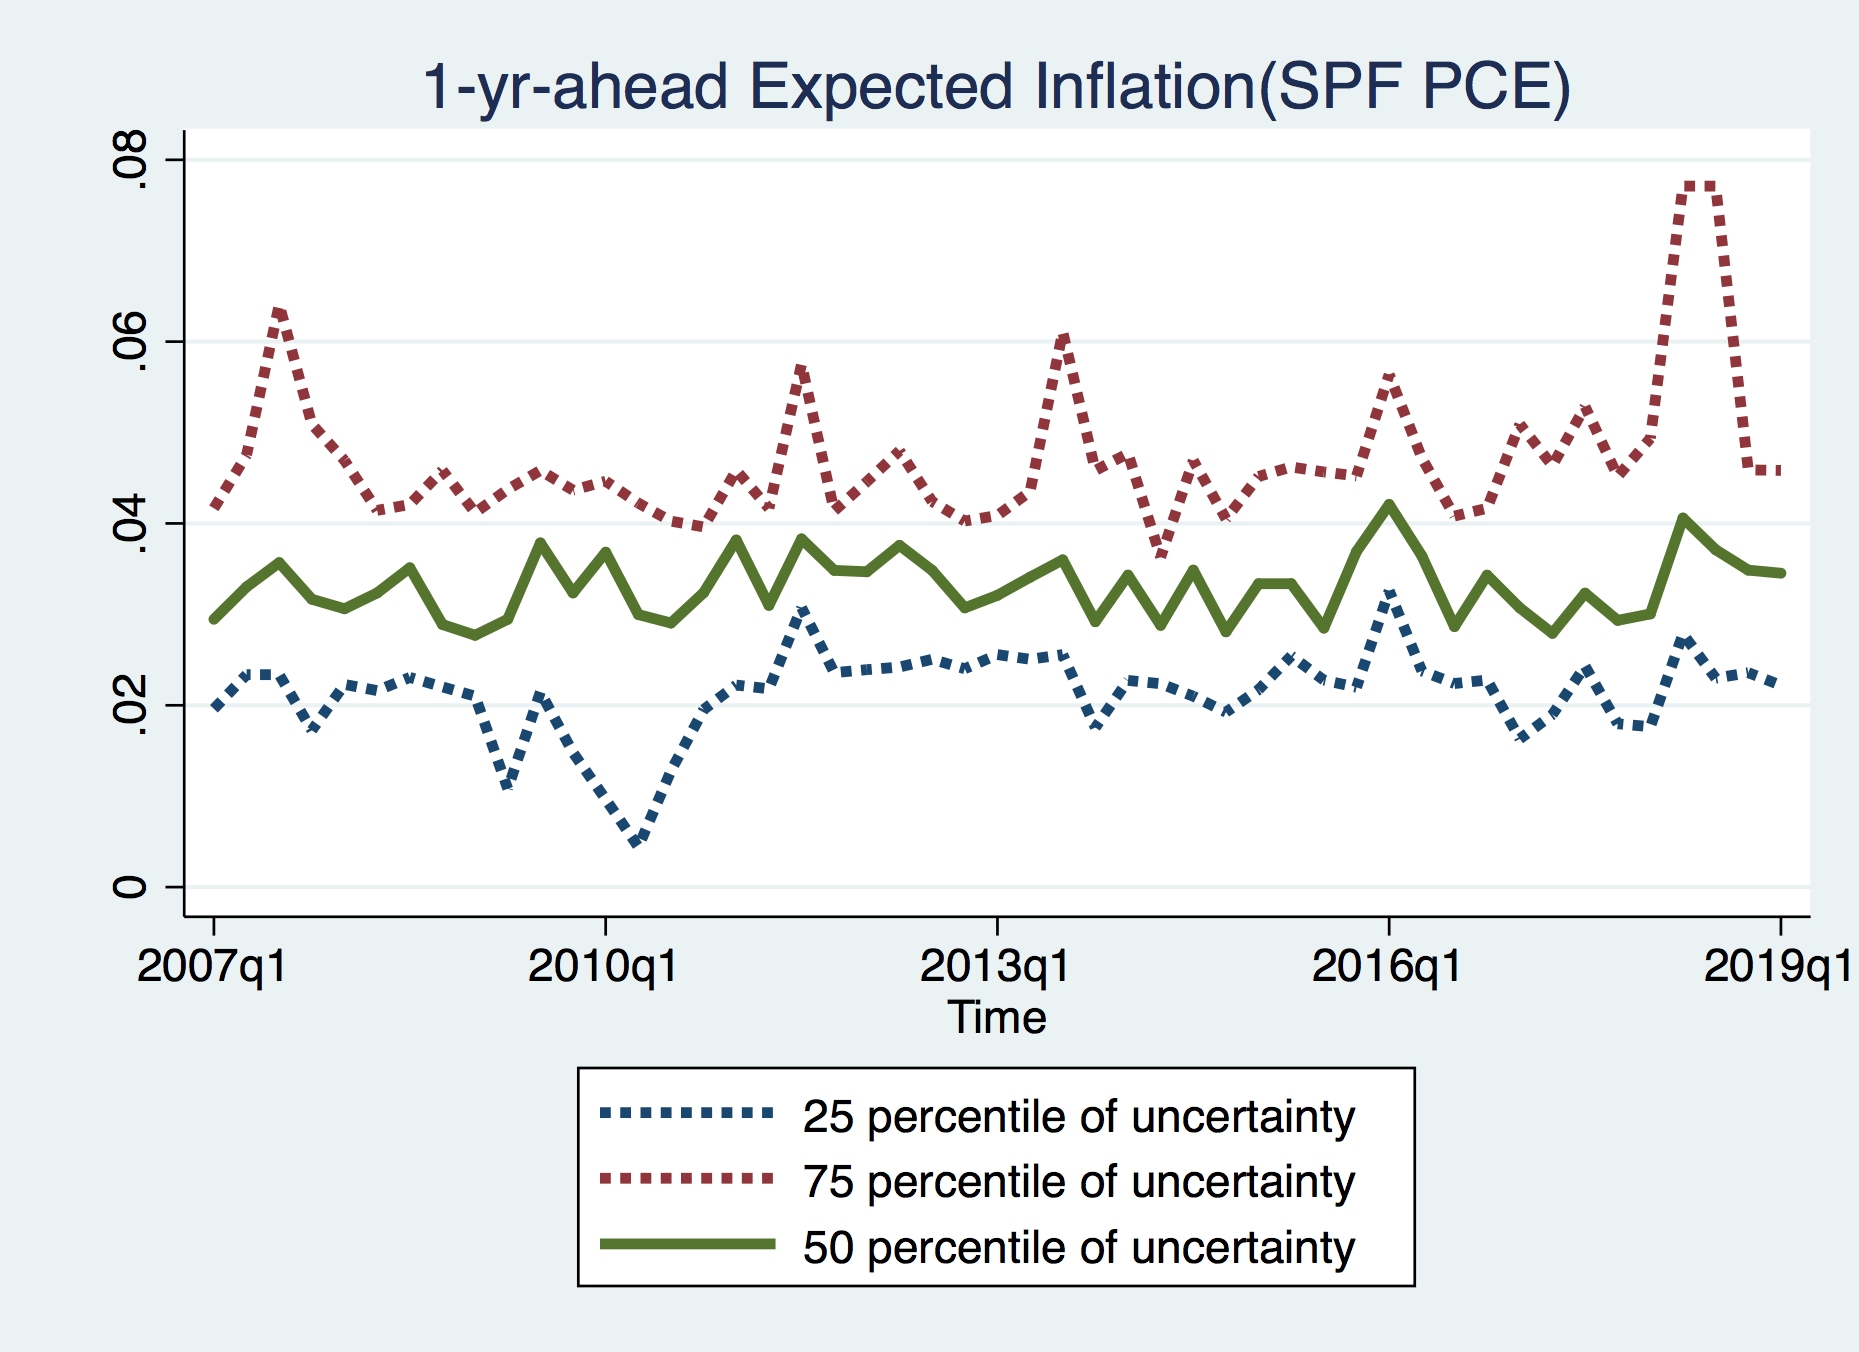
\includegraphics[width=0.33\textwidth]{figuresDraft/IQRvarPCEQ.png}
\smallskip
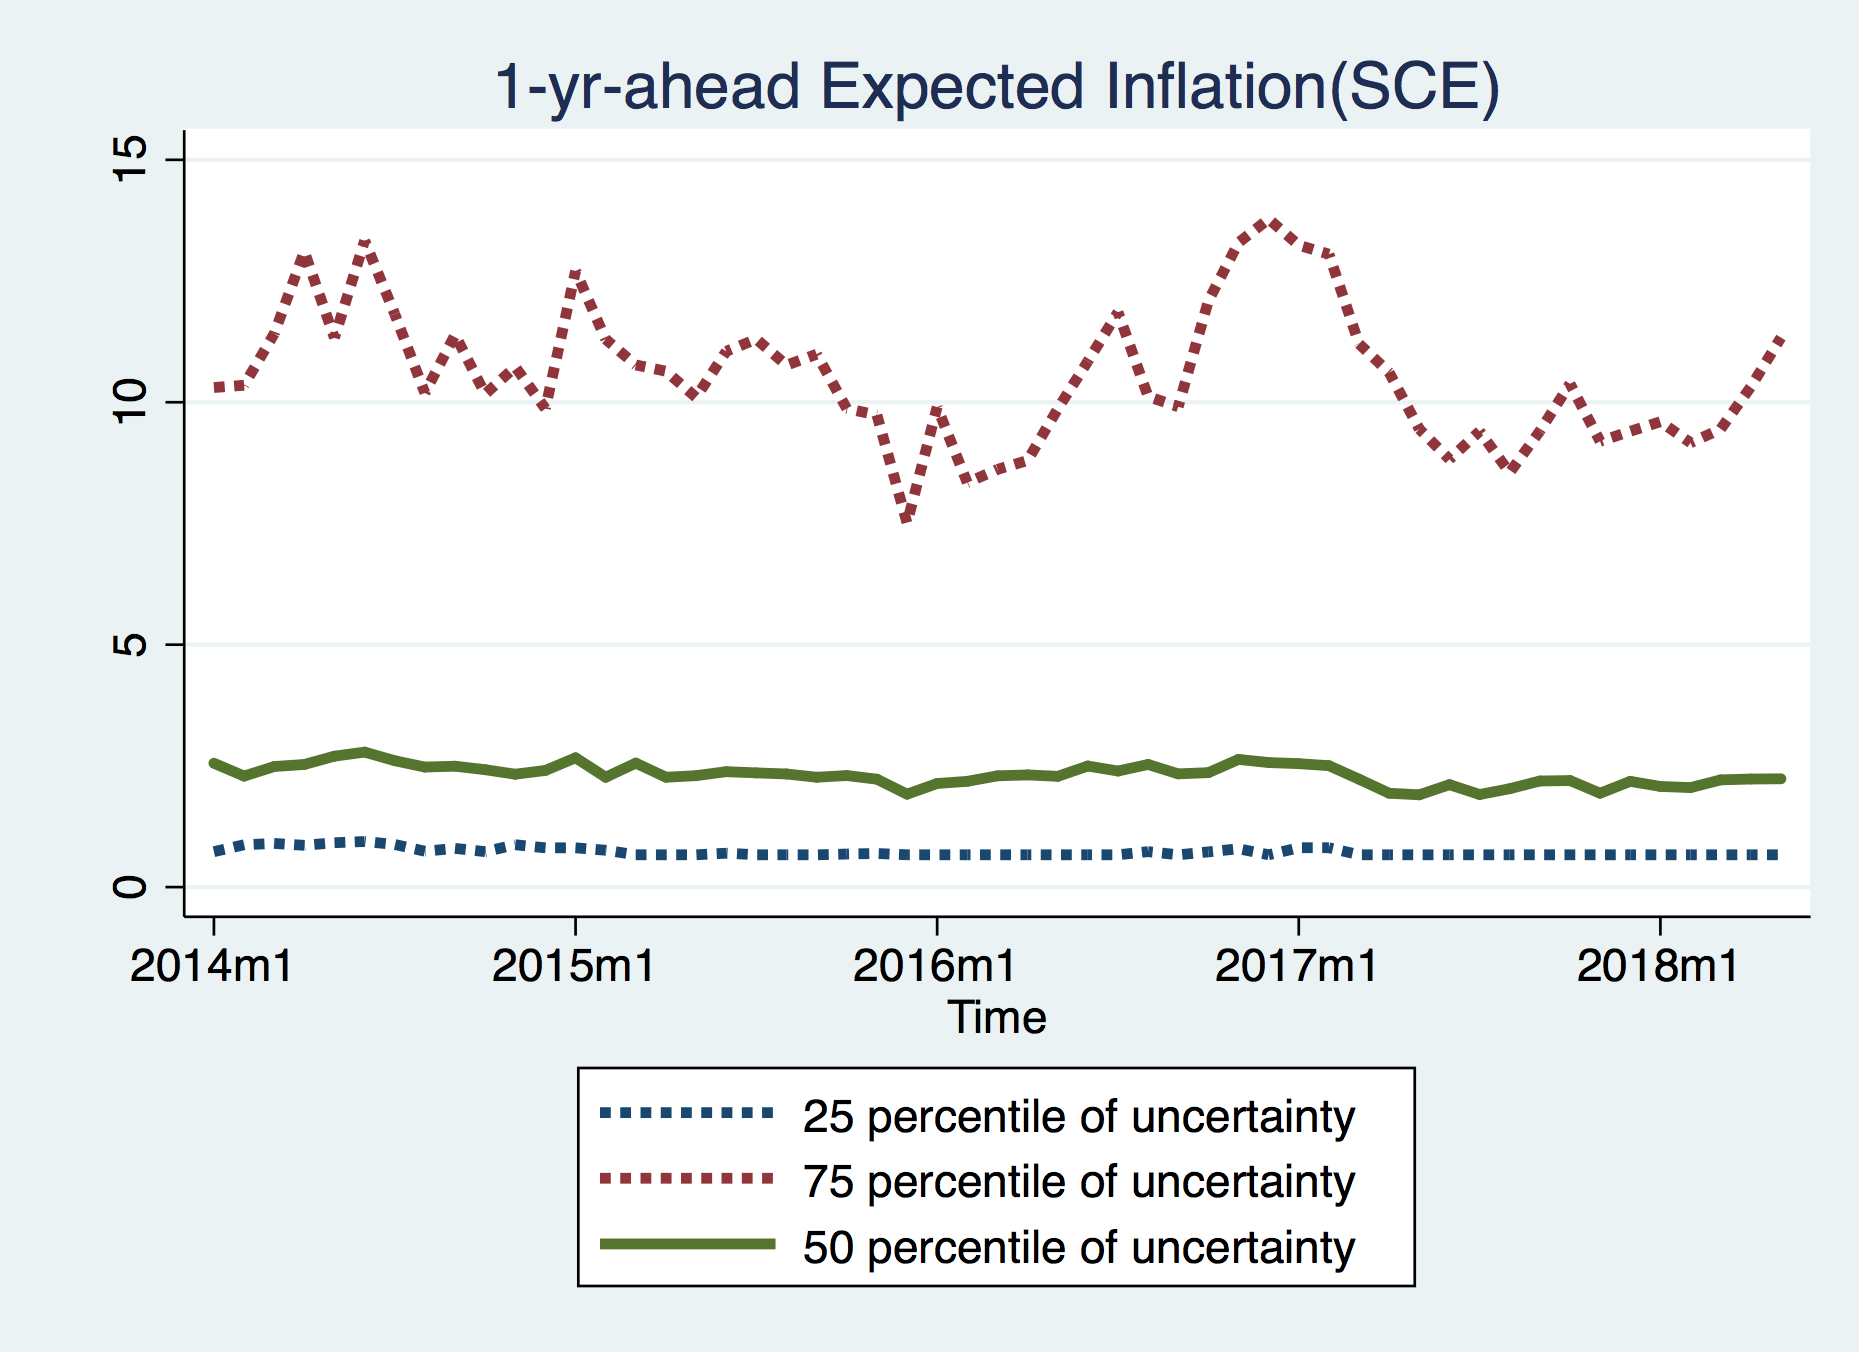
\includegraphics[width=0.33\textwidth]{figuresDraft/IQRvarSCEM.png}
\end{figure}
\end{frame}


\begin{frame}{Distribution of Uncertainty}
\begin{figure}
		\label{Unceratitny_Histogram}
	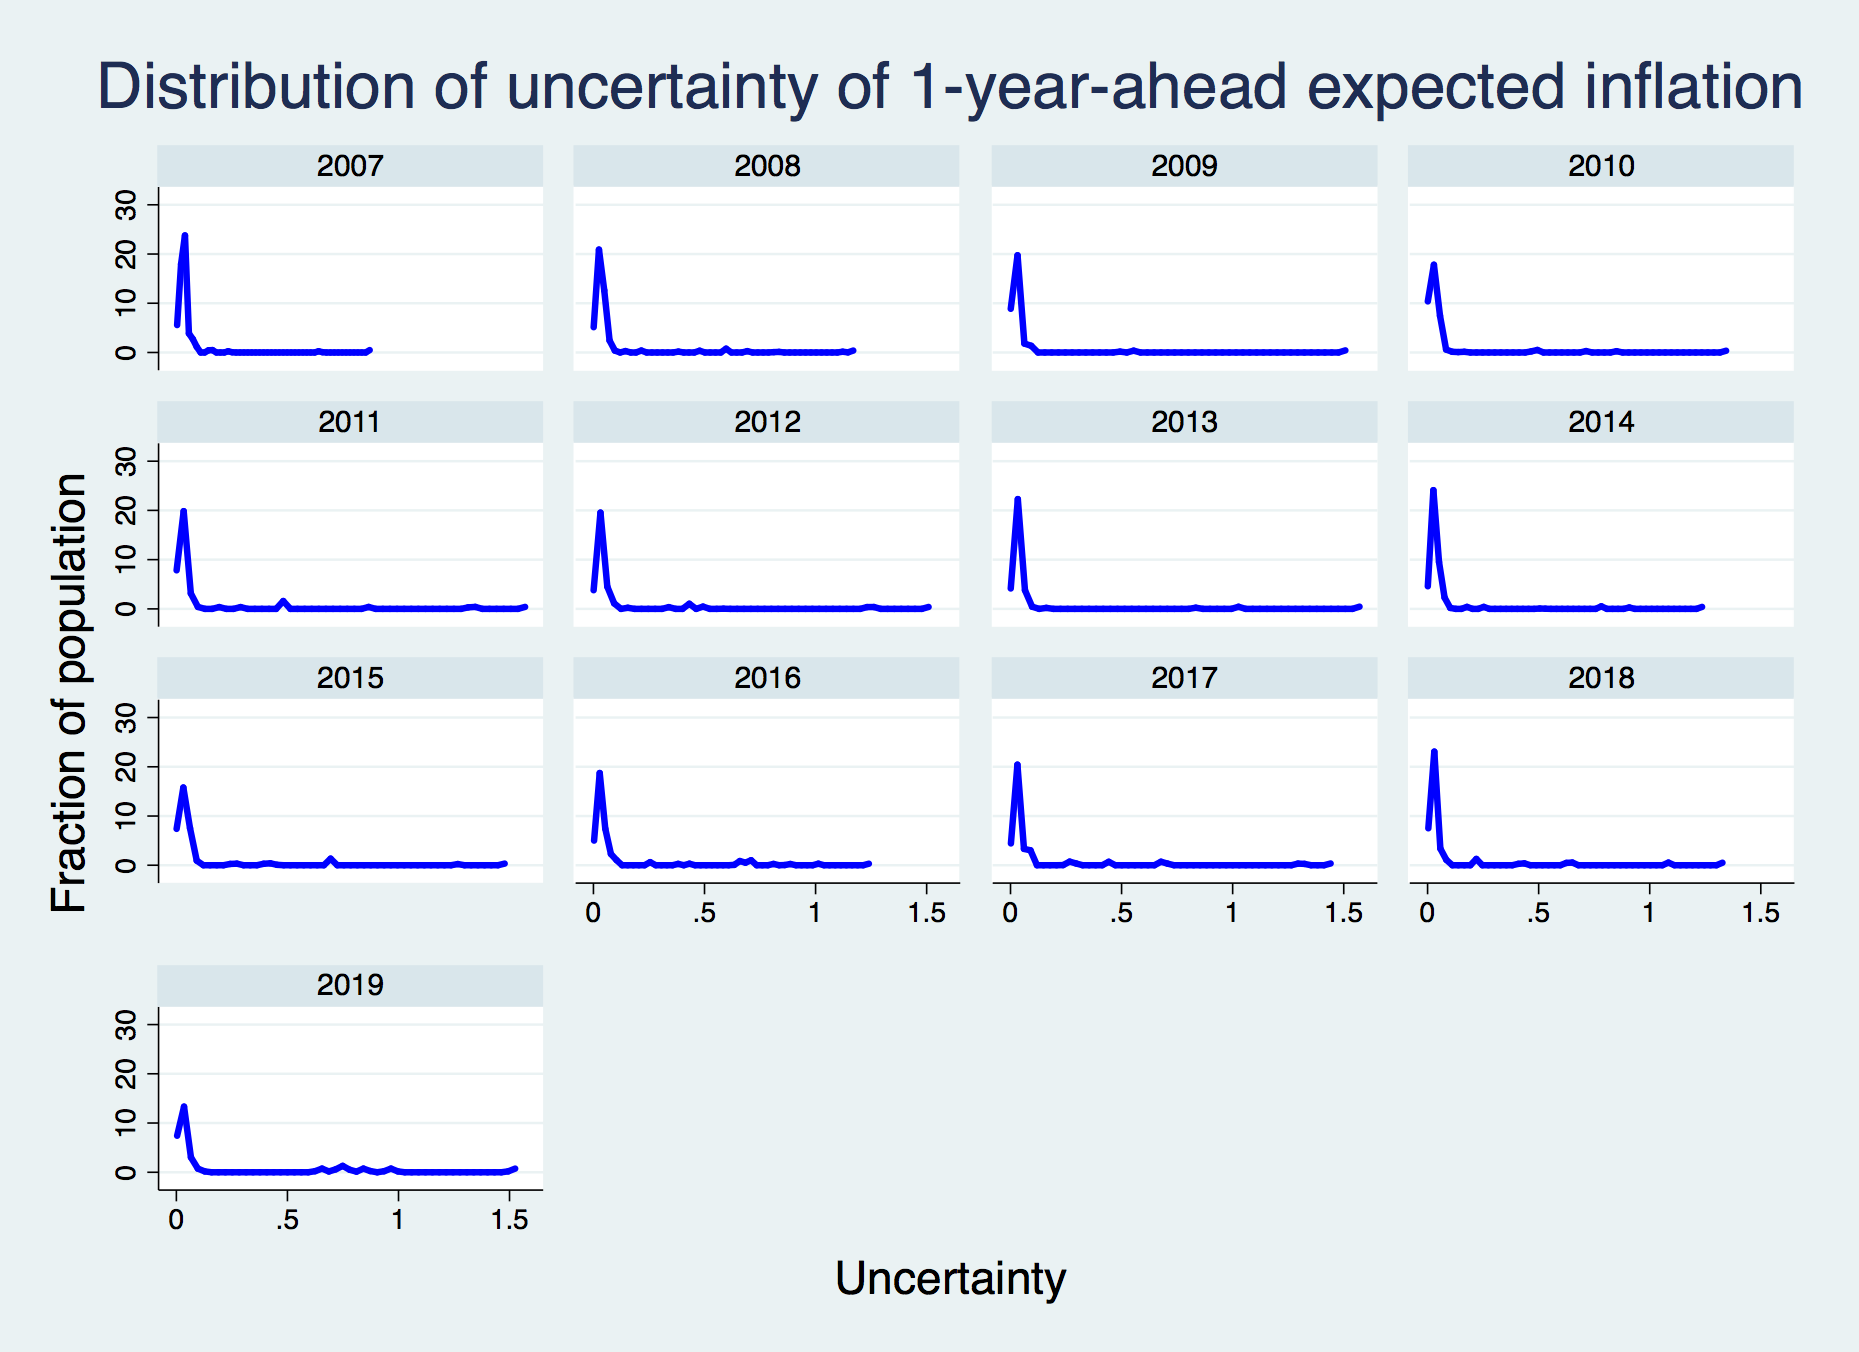
\includegraphics[width=0.33\textwidth]{figuresDraft/PRCCPIVar1_hist.png}  
\smallskip
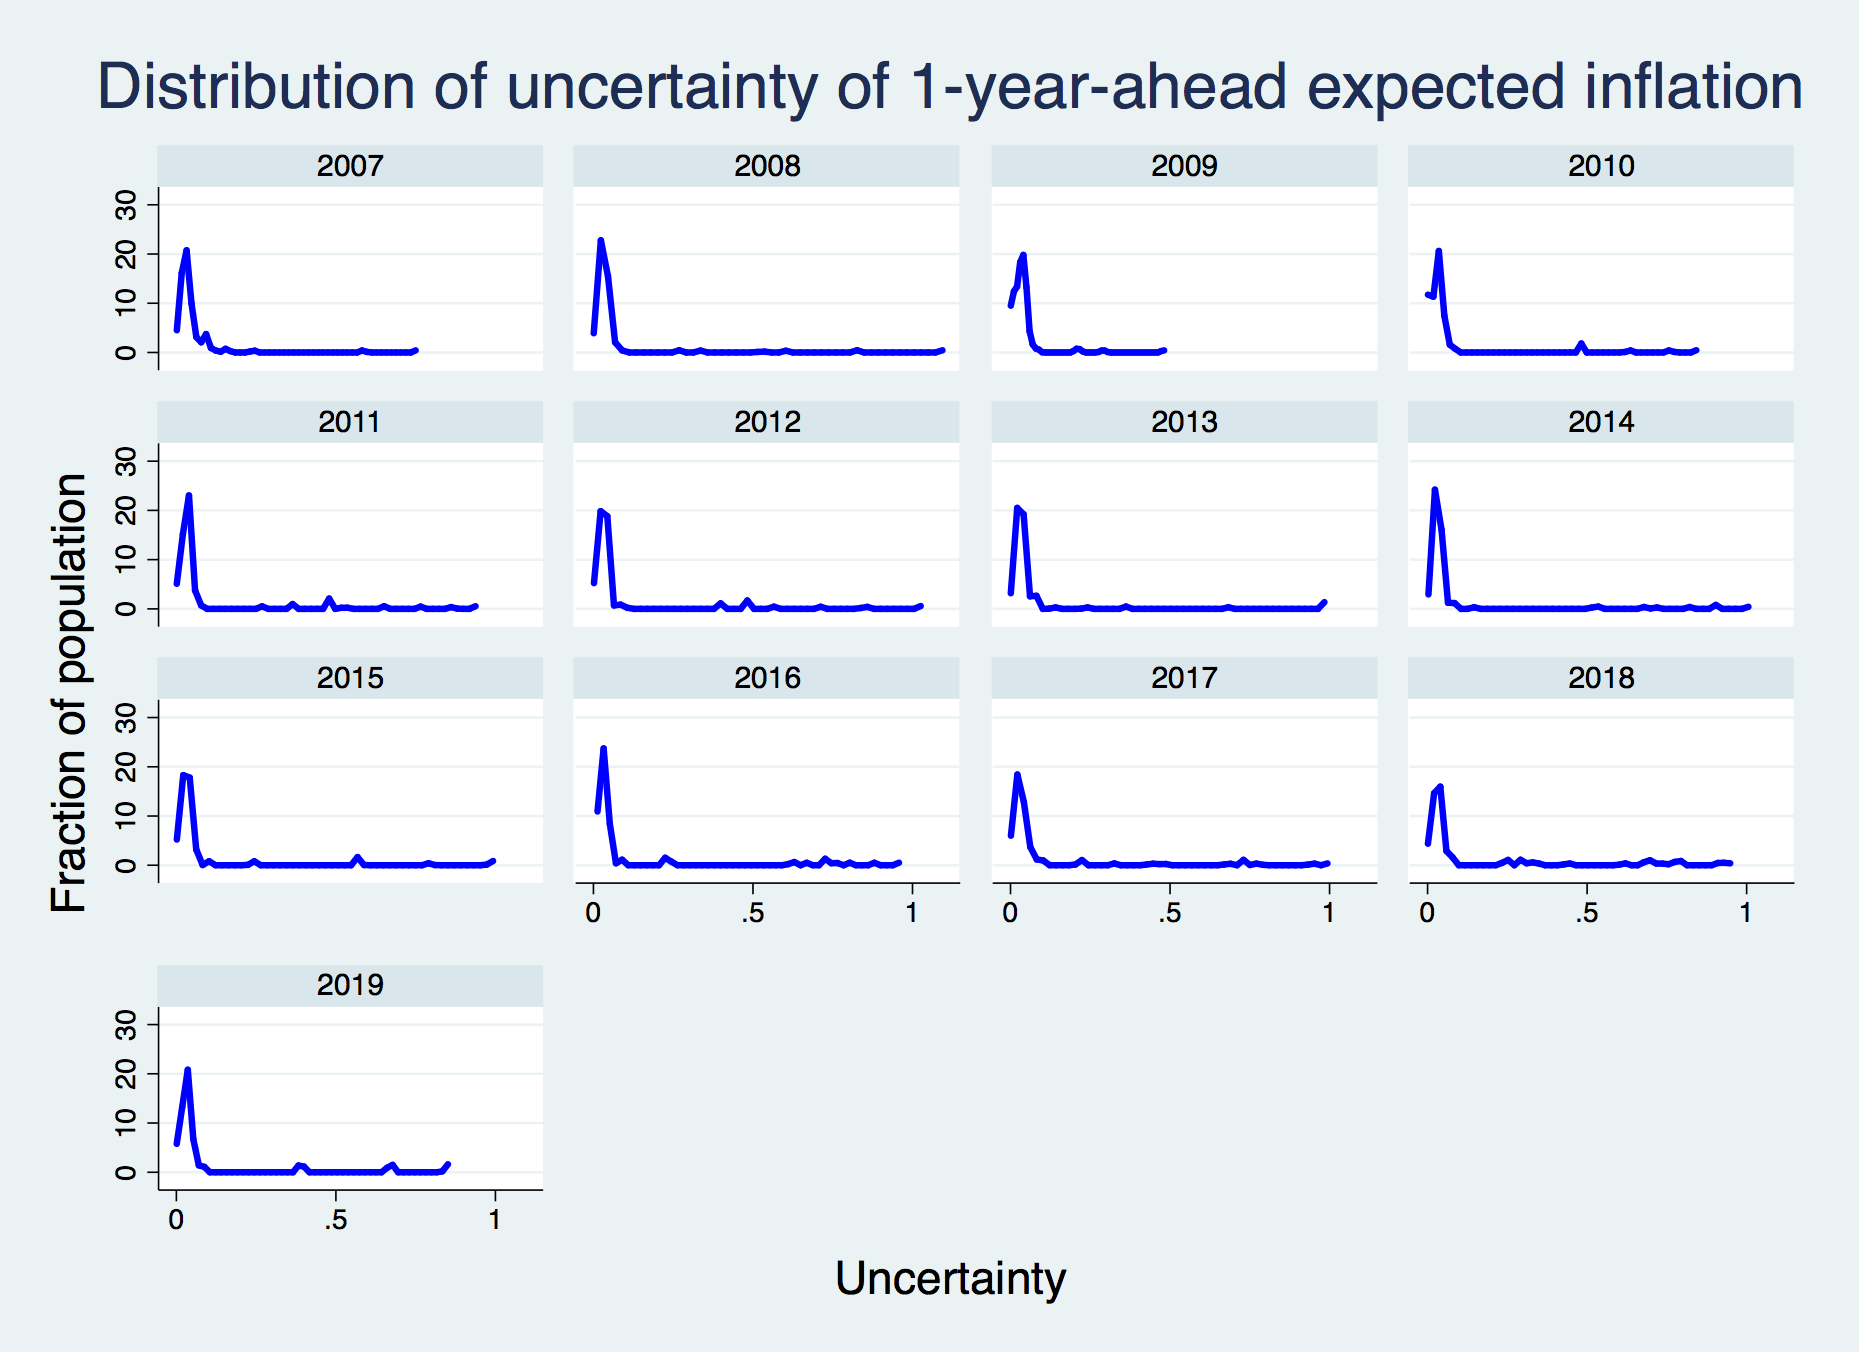
\includegraphics[width=0.33\textwidth]{figuresDraft/PRCPCEVar1_hist.png}  
\smallskip
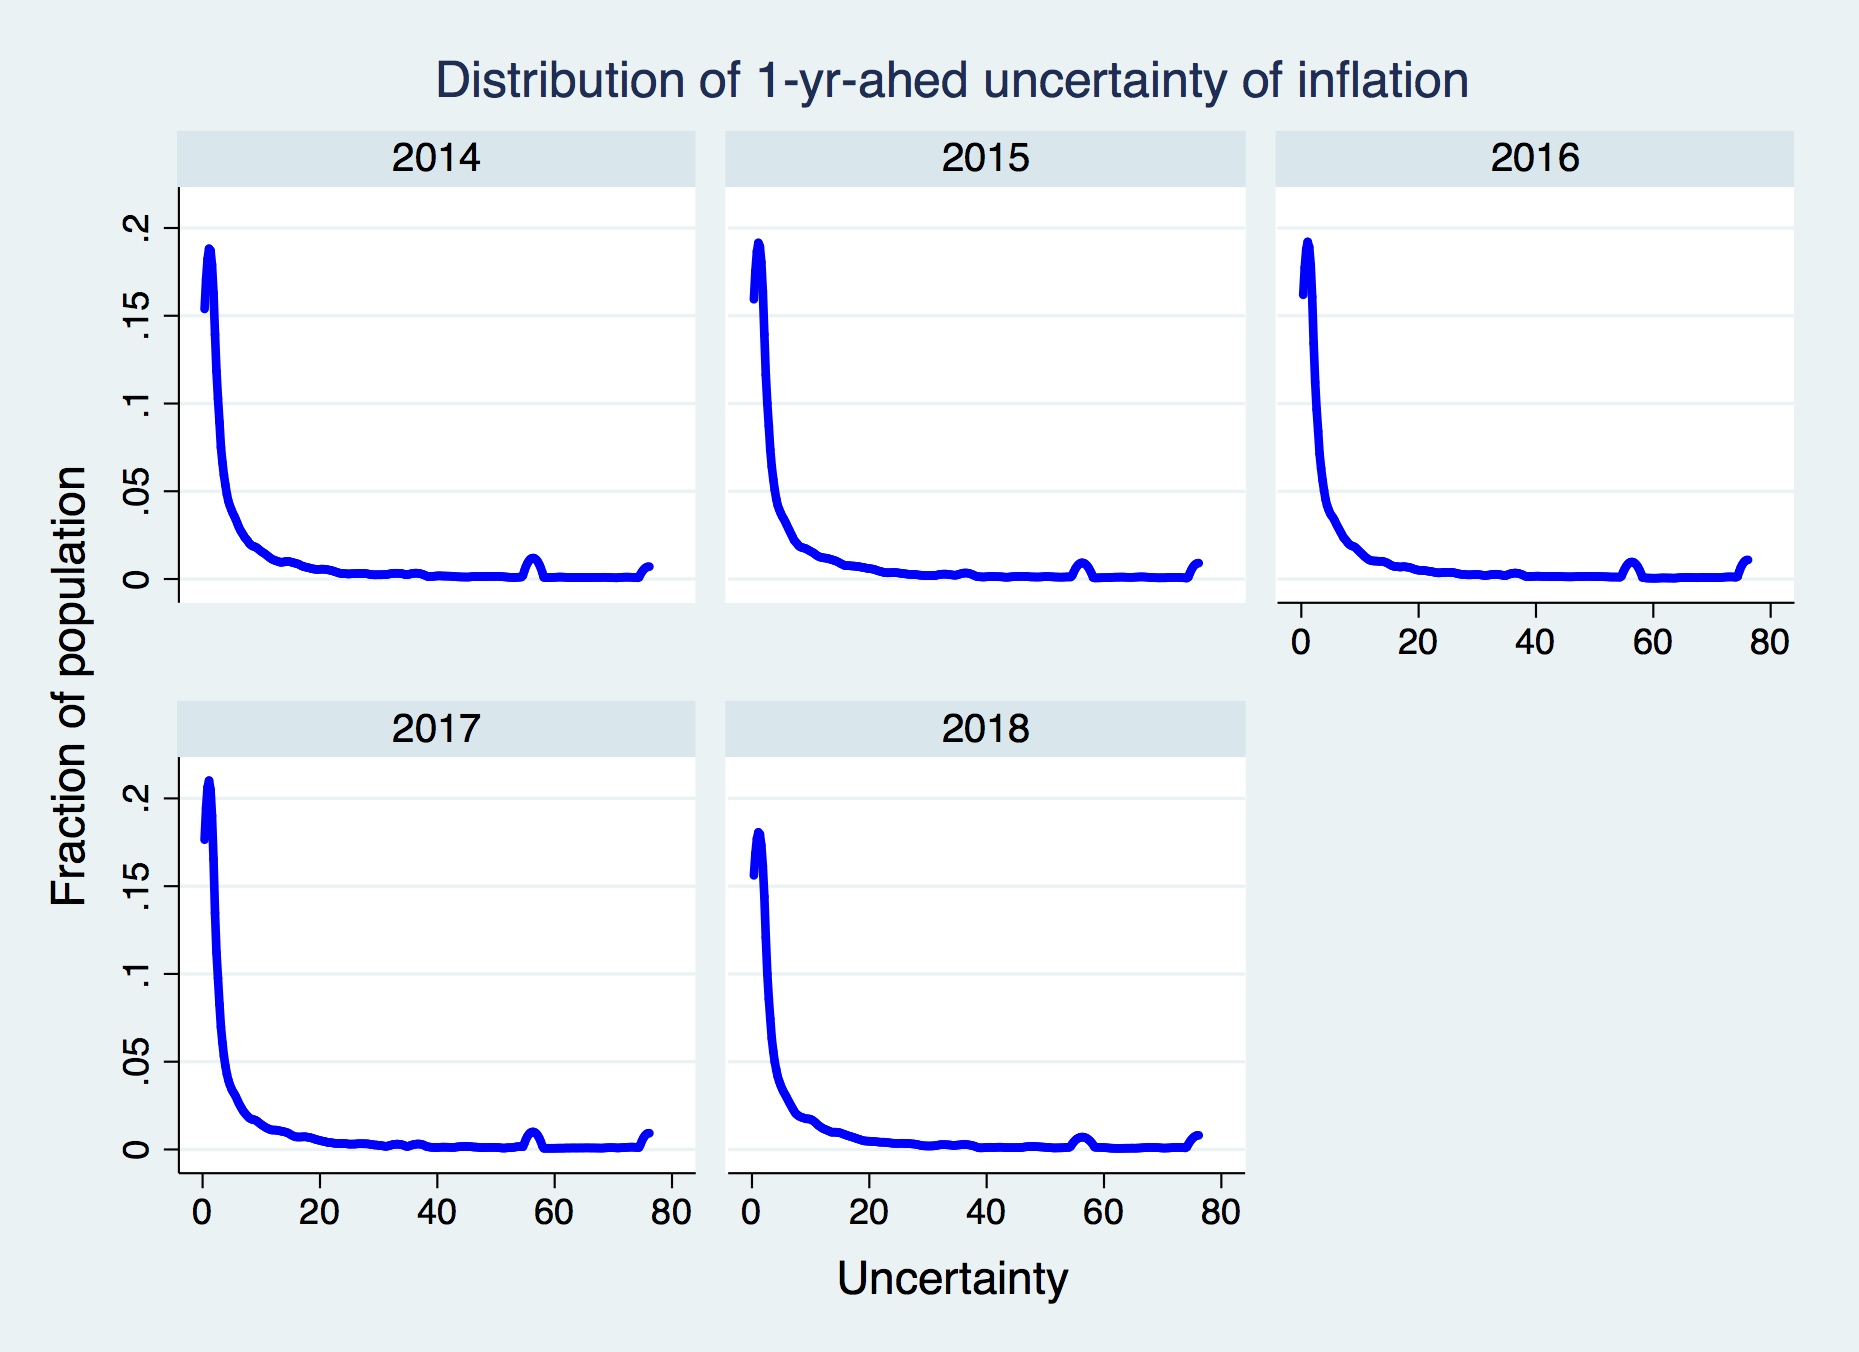
\includegraphics[width=0.33\textwidth]{figuresDraft/SCEvar_hist.png}  
\end{figure}
\end{frame}


\begin{frame}{Distribution of Revision in Forecast}
\begin{figure}
	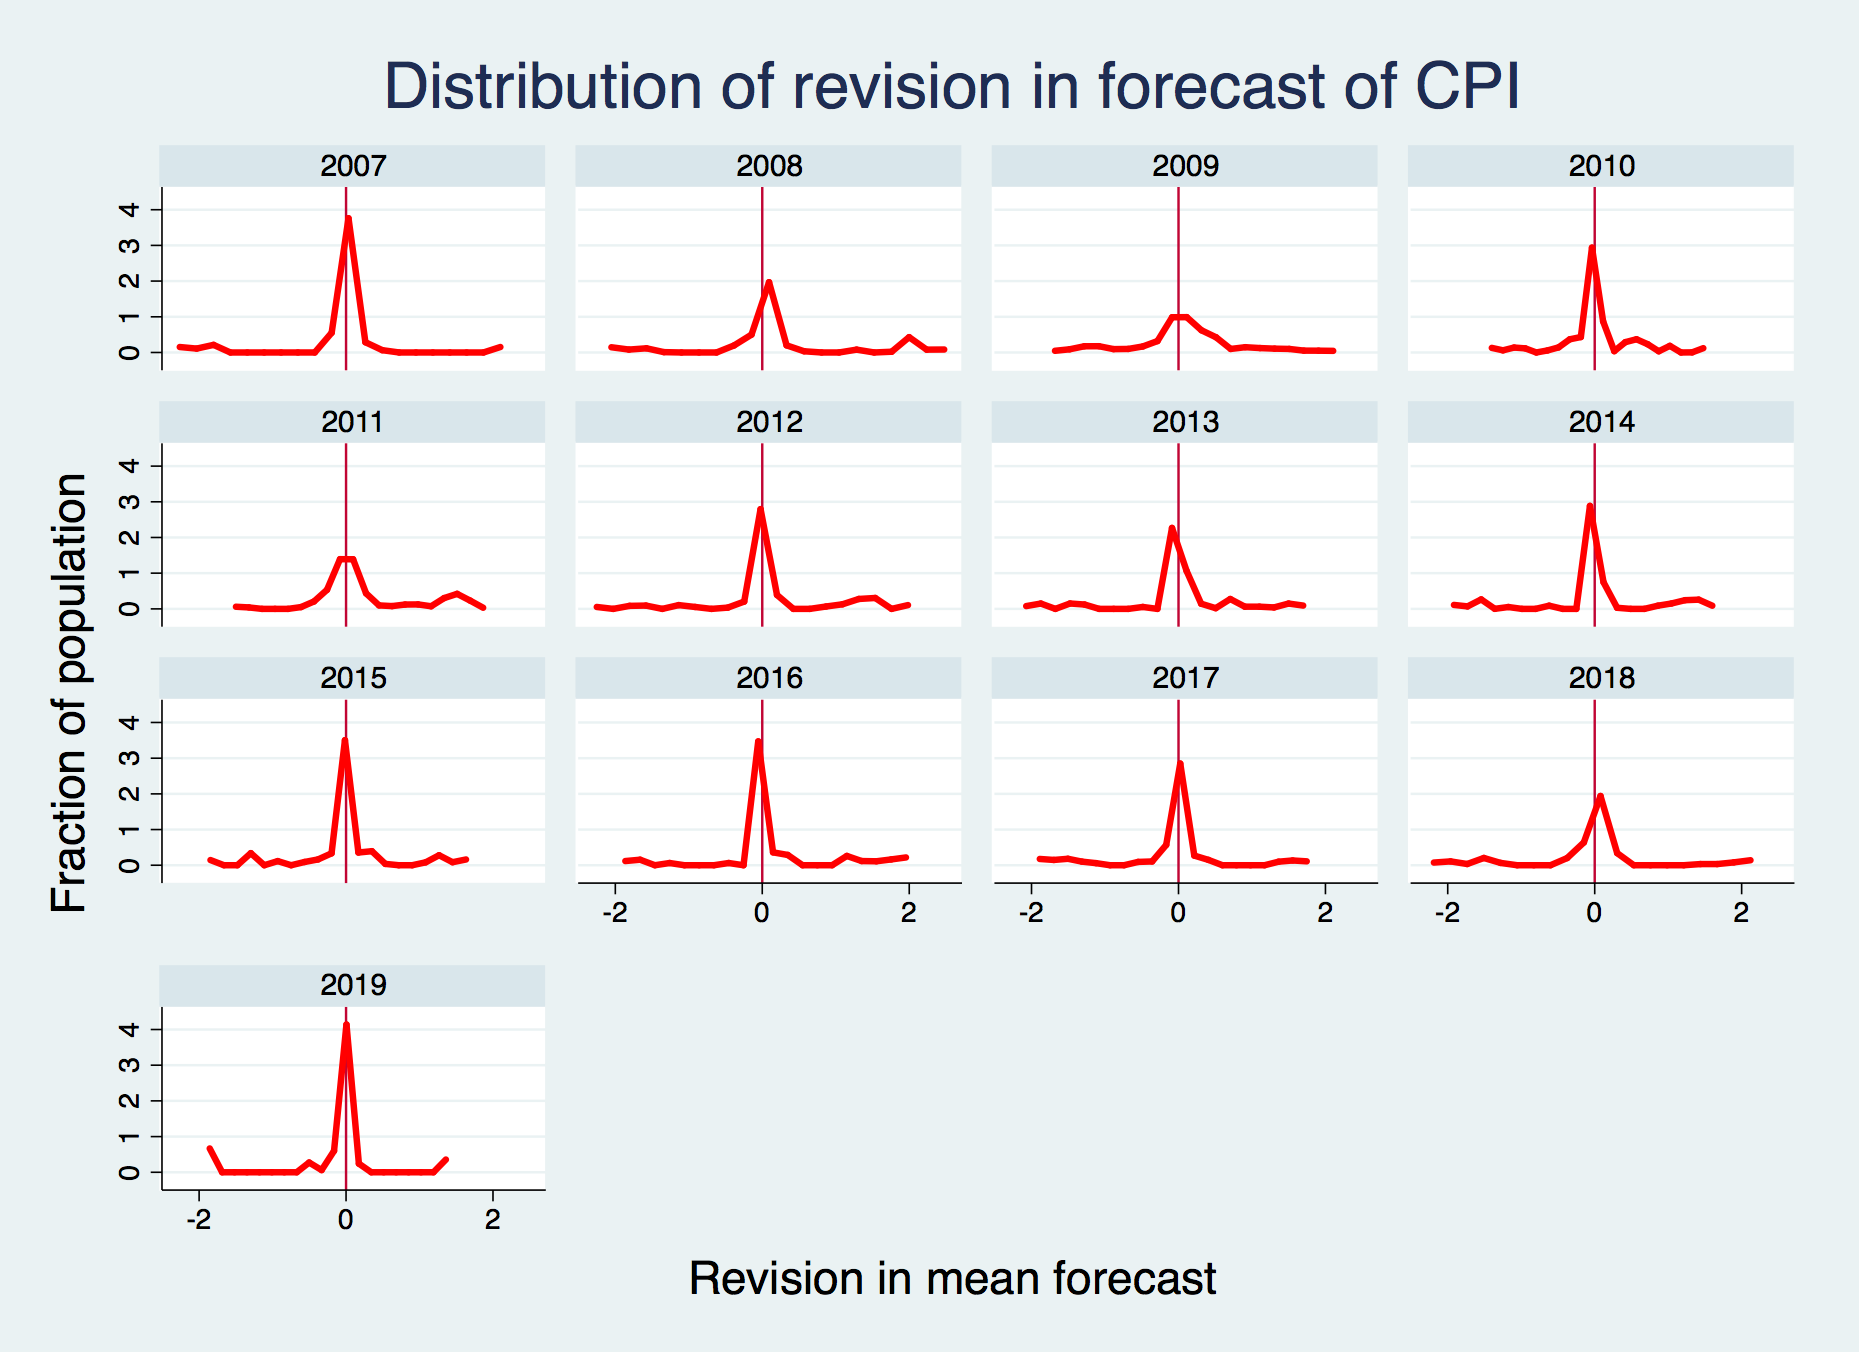
\includegraphics[width=0.5\textwidth]{figuresDraft/PRCCPIMean01_rv_true_hist.png} 
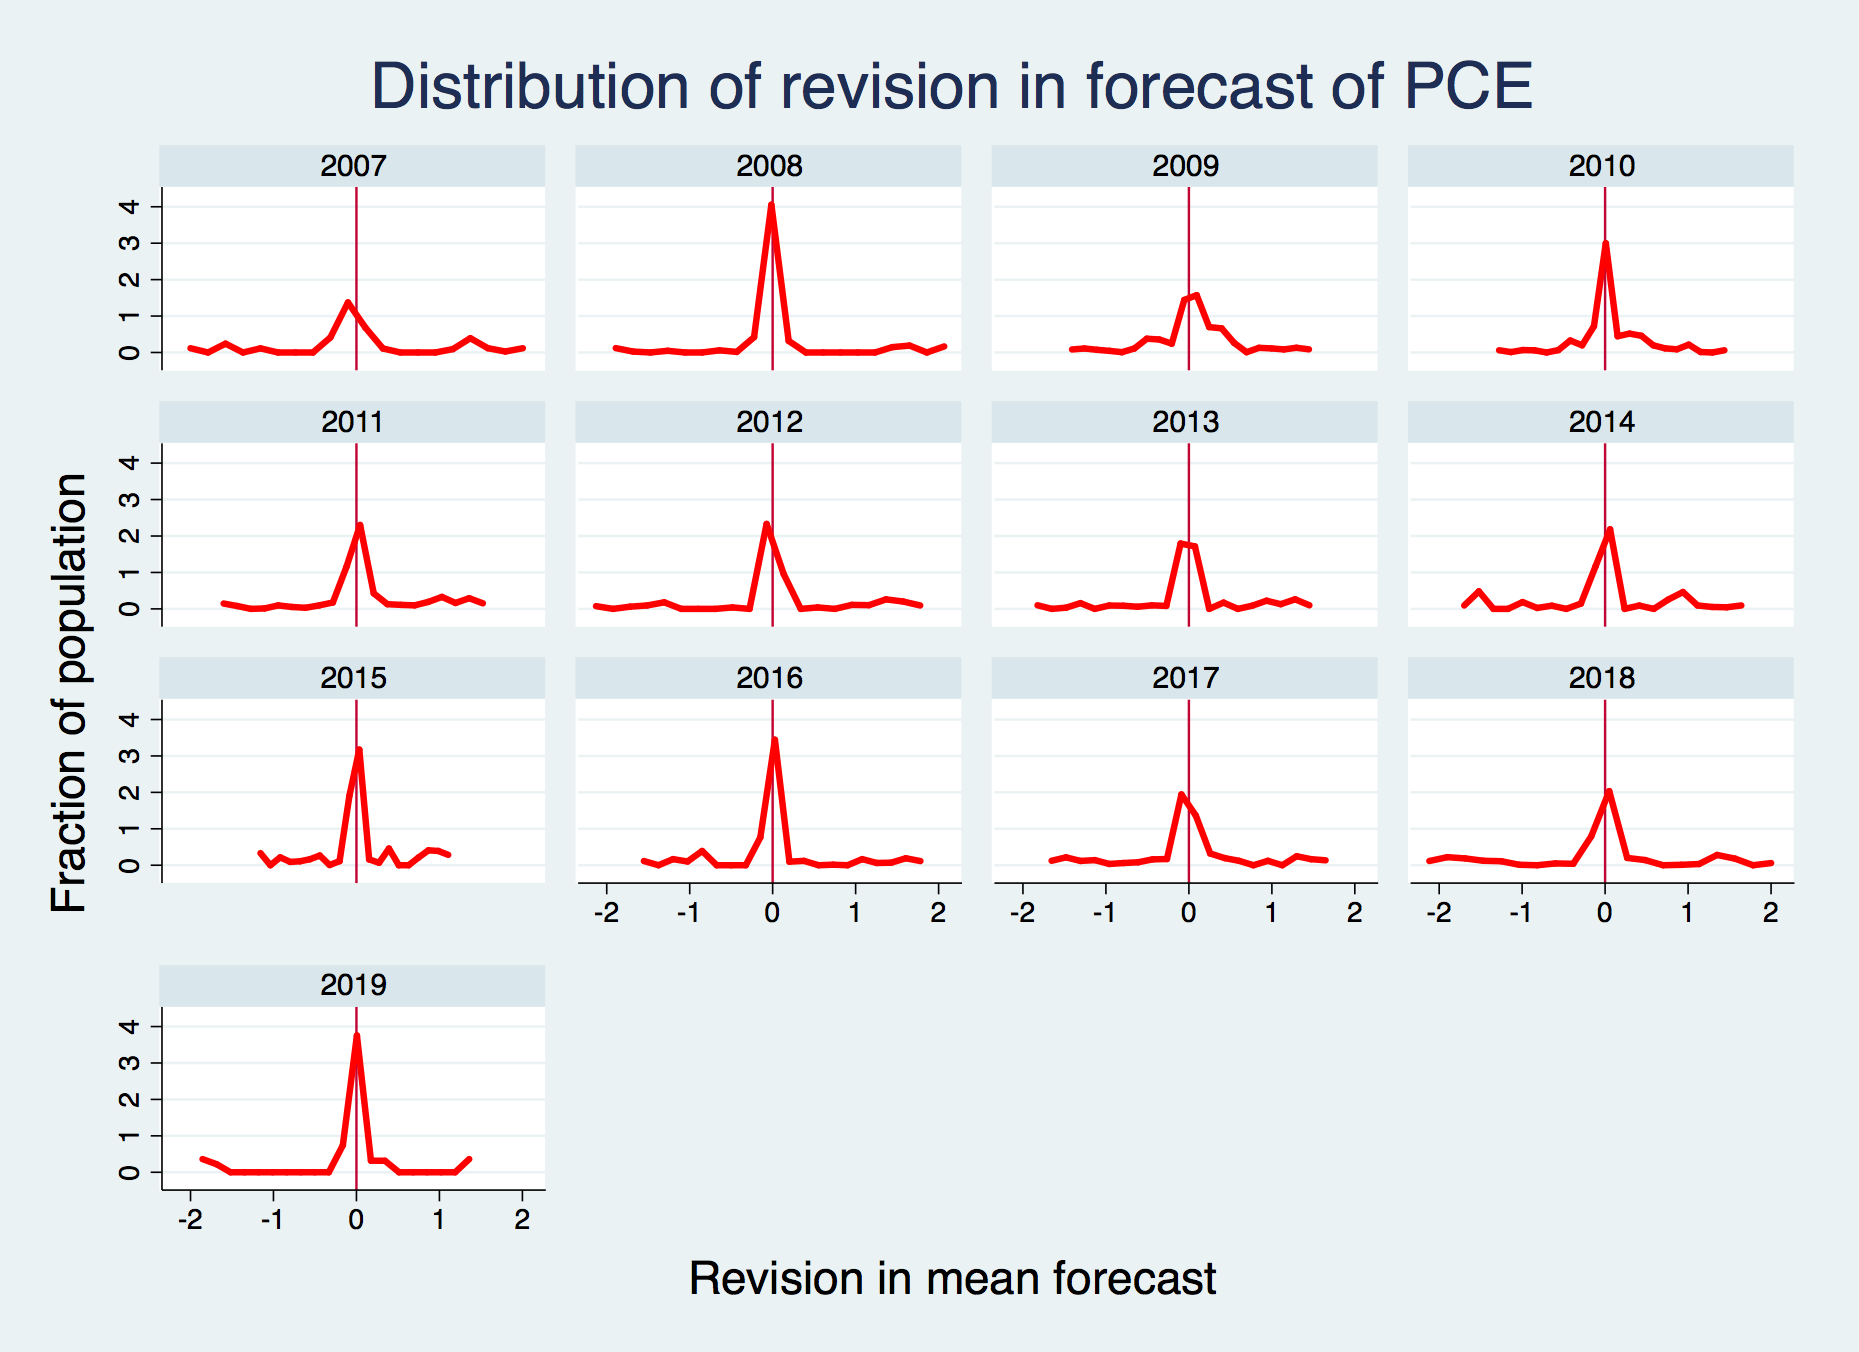
\includegraphics[width=0.5\textwidth]{figuresDraft/PRCPCEMean01_rv_true_hist.png} 
\end{figure}
\end{frame}


\begin{frame}{Distribution of Revision in Uncertainty}
\begin{figure}
	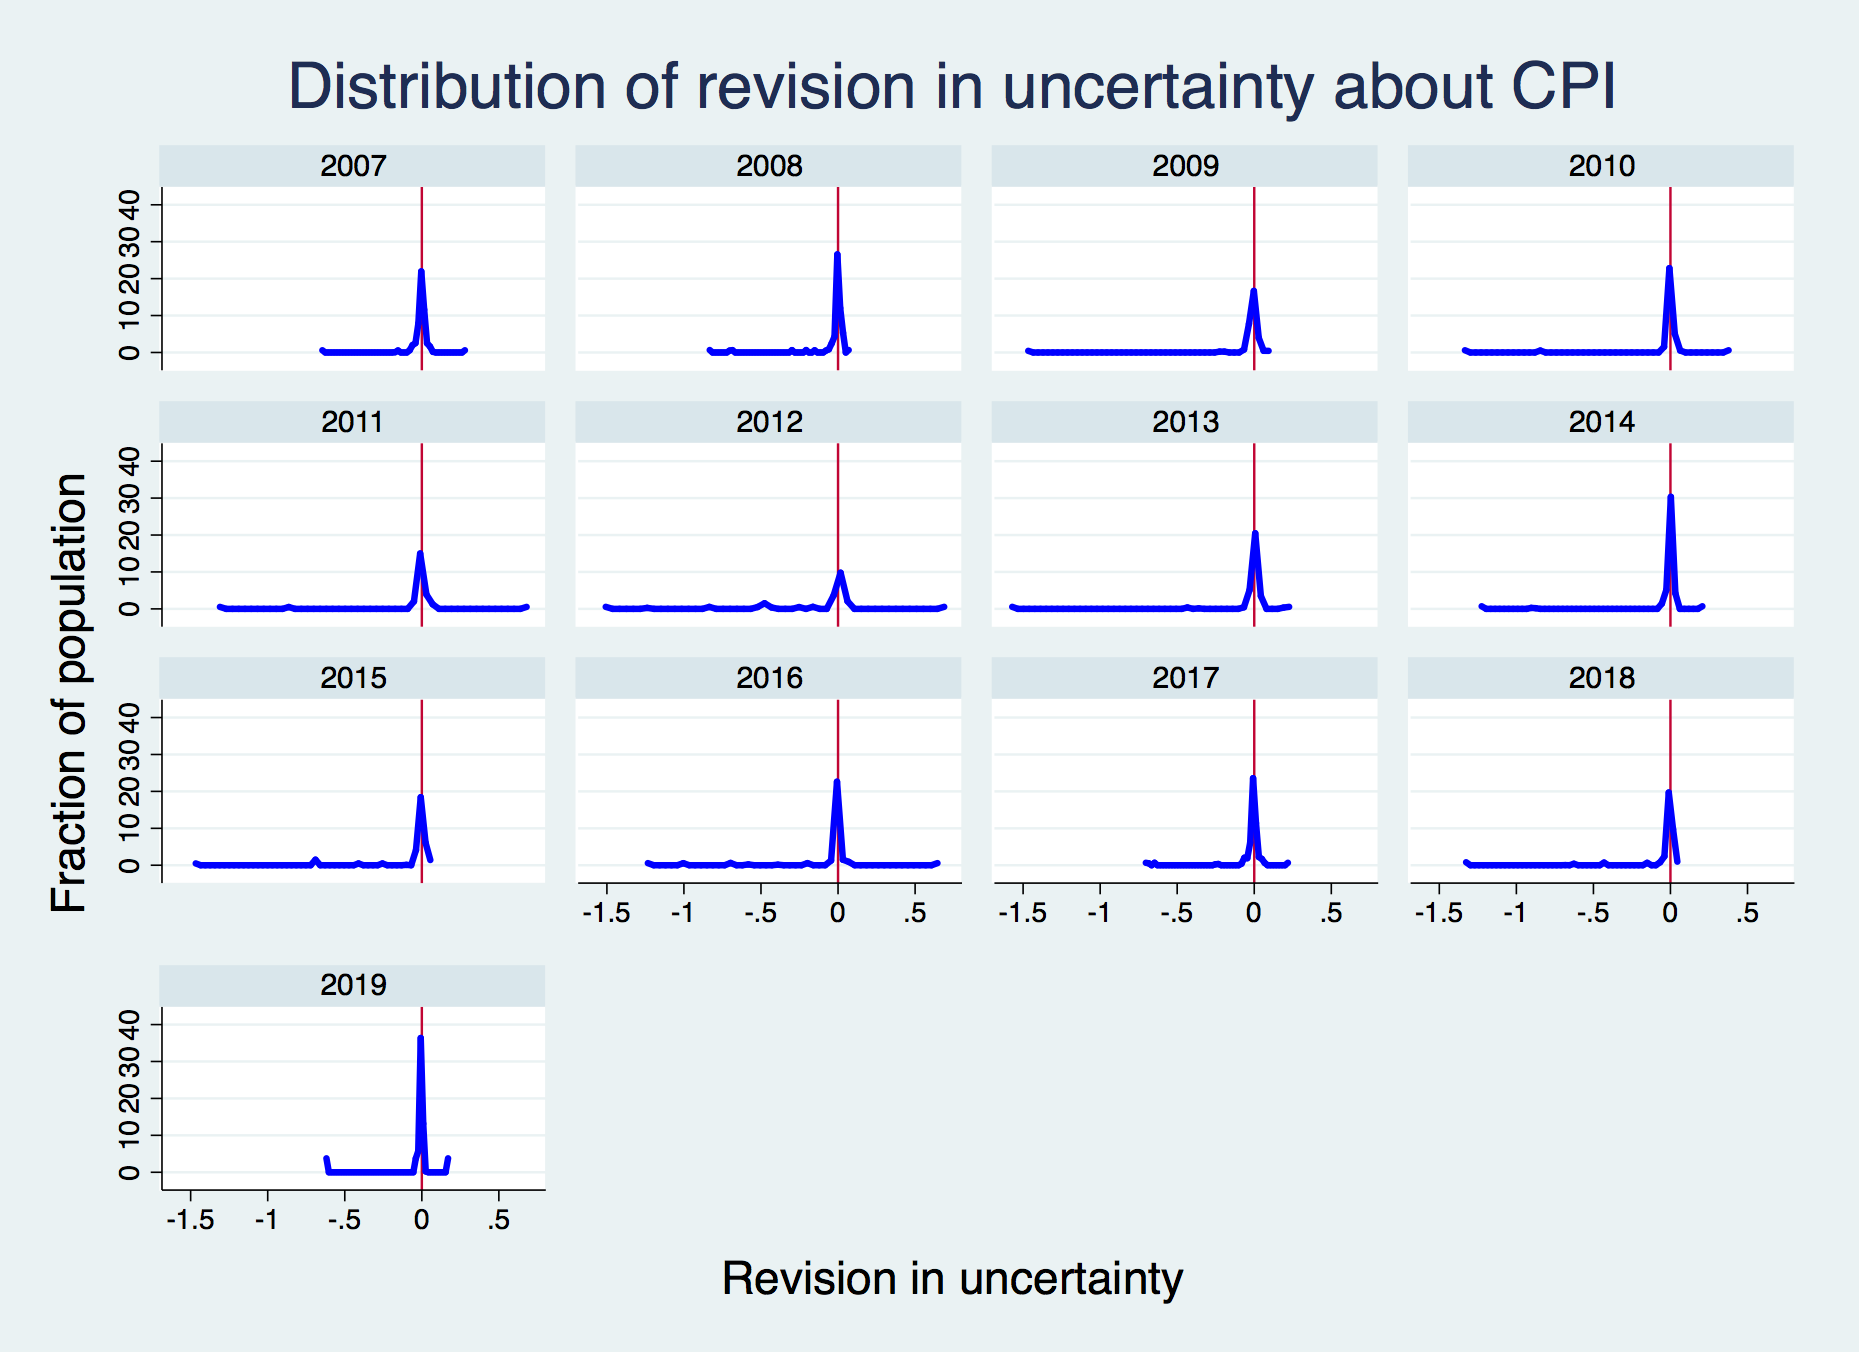
\includegraphics[width=0.5\textwidth]{figuresDraft/PRCCPIVar01_rv_true_hist.png}  
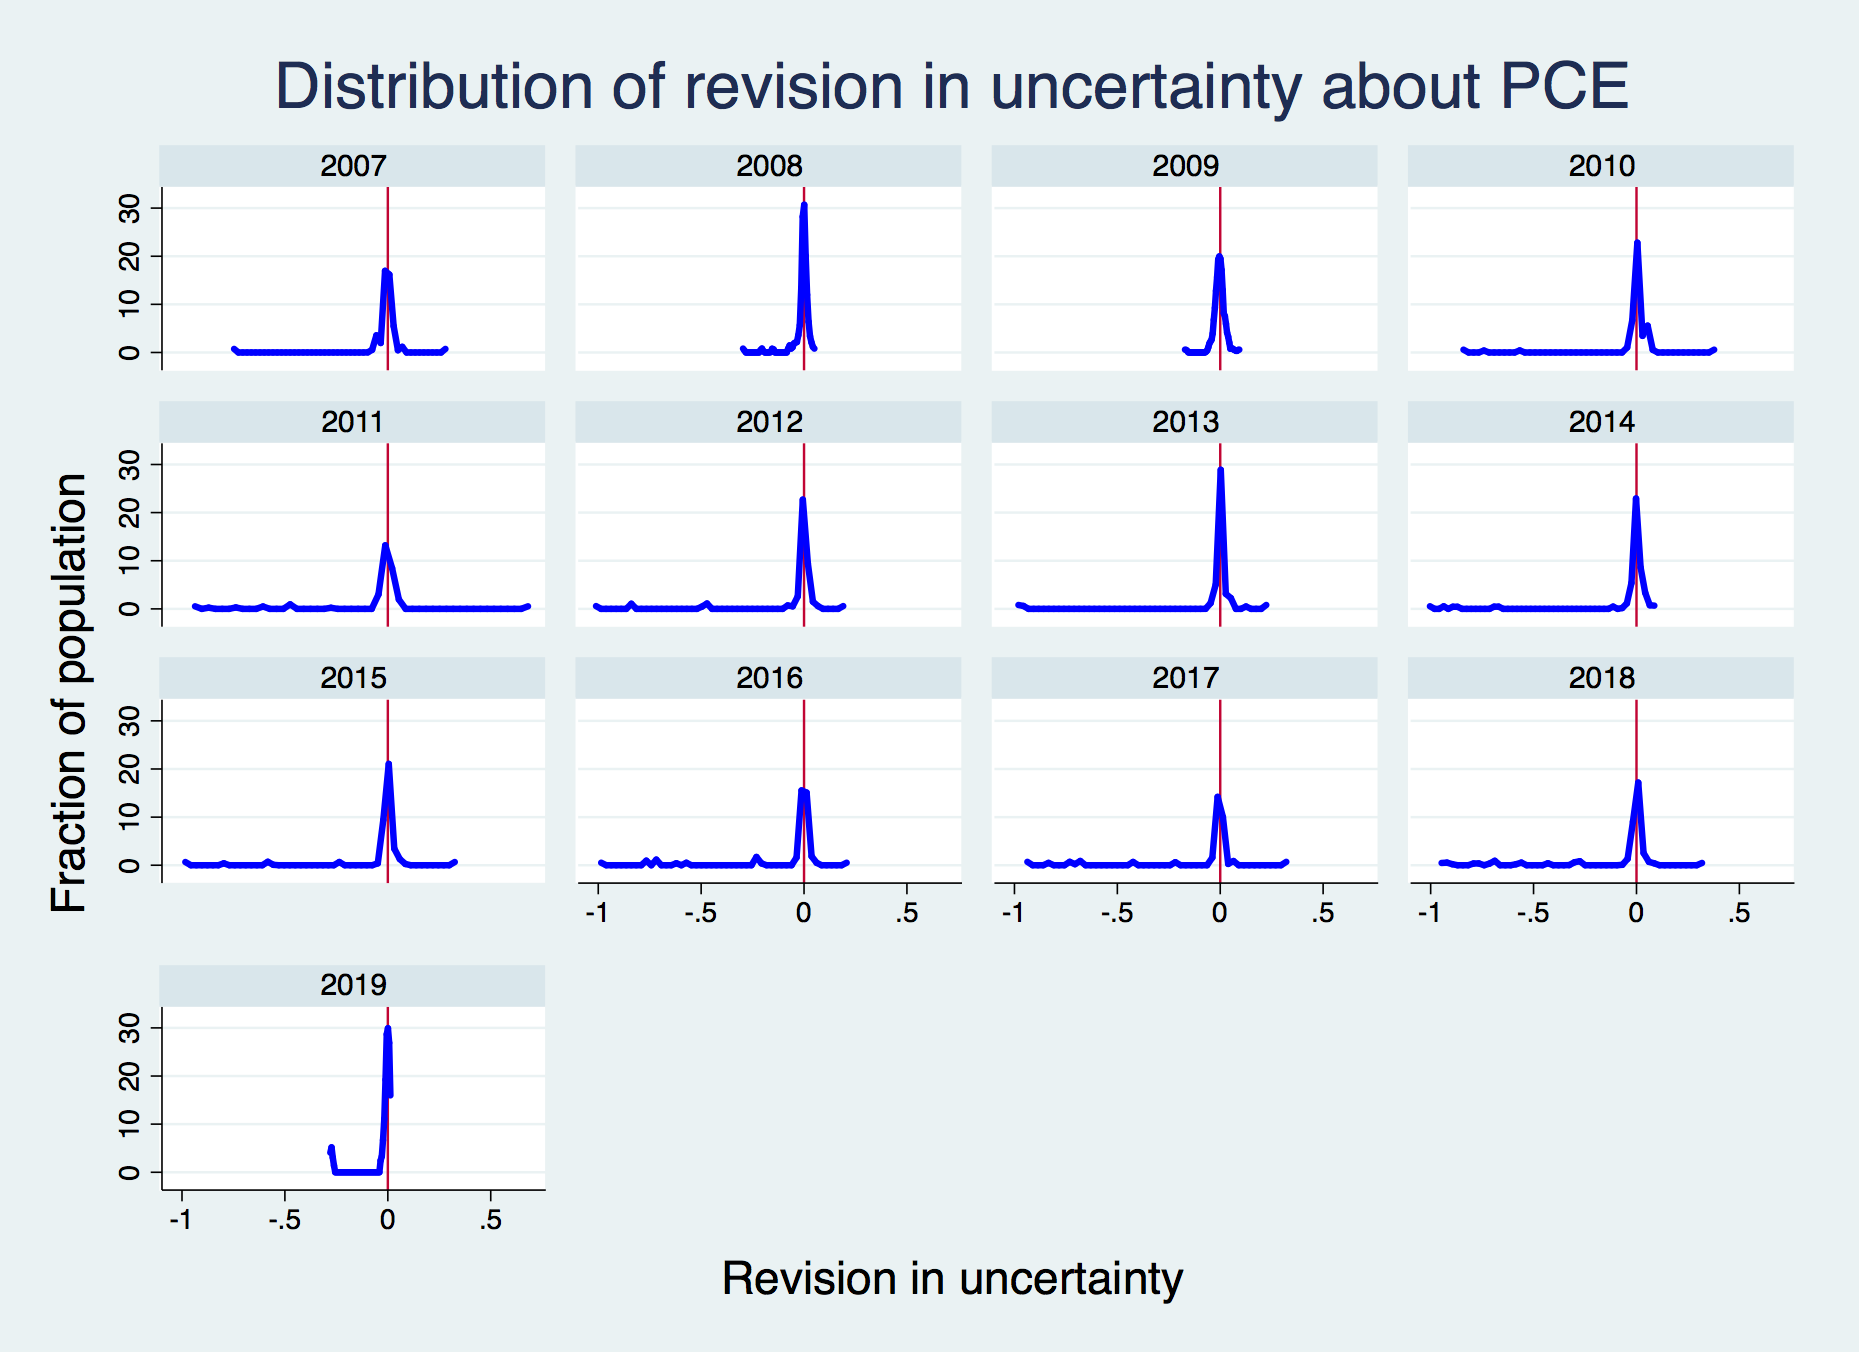
\includegraphics[width=0.5\textwidth]{figuresDraft/PRCPCEVar01_rv_true_hist.png} 
\end{figure}
\end{frame}



\section{Empirical Results}

\begin{frame}{Empirical execution}

\begin{itemize}

\item \textbf{Density Estimation}: generalized beta estimation, \cite{engelberg2009comparing}
 \item \textbf{Identification of Shocks}: following \cite{coibion2012can} and monetary policy shocks. 
\end{itemize}

\end{frame}

\subsection{Test of Null Hypothesis of Rational Expectation}

\begin{frame}{Tests of rationality using forecast errors}
	\begin{adjustbox}{totalheight=0.9\textheight}
	\label{NullTestTable}
	\centering 
	\begin{tabular}{llll}
		\hline 
		& SPF CPI          & SPF PCE          & SCE            \\
		\hline 
		\multicolumn{4}{l}{Test 1: Unbiasedness}                                                           \\
		\hline 
		Constant                            & 0.122***         & 0.586***         & 2.220***       \\
		& (0.017)          & (0.061)          & (0.019)        \\
		\hline 
		N                                   & 4697             & 1208             & 67380          \\
		\hline 
		\multicolumn{4}{l}{Test 2: FE does not depend on past information}                                  \\
		\hline 
		Forecast 1-yr before                & 0.307***         & 0.586***         & NA             \\
		& (0.020)          & (0.061)          & NA             \\
		Constant                            & -0.655***        & -0.777***        & NA             \\
		& (0.060)          & (0.116)          & NA             \\
		\hline 
		N                                   & 3429             & 1208             & NA             \\
		$R^2$                 & 0.0721           & 0.118            & NA             \\
		\hline 
		\multicolumn{4}{l}{Test 3: FEs of non-overlapping forecast horizons not serially correlated} \\
		\hline 
		Forecast Error 1-year before        & 0.0756***        & 0.0503***        & NA             \\
		& (0.020)          & (0.035)          & NA             \\
		Constant                            & 0.145***         & 0.275***         & NA             \\
		& (0.021)          & (0.035)          & NA             \\
		\hline 
		N                                   & 3356             & 1208             & NA             \\
		$R^2$                   & 0.00591          & 0.00264          & NA             \\
		\hline 
		\multicolumn{4}{l}{Test 4: Overlapping FEs are only weakly serially correlated}                          \\
		\hline 
		Forecast Error 1-q before           & 0.657***         & 0.834***         & 0.297***       \\
		& (0.025)          & (0.037)          & (0.021)        \\
		Forecast Error 2-q before           & 0.0282           & -0.0858          & 0.308***       \\
		& (0.027)          & (0.048)          & (0.046)        \\
		Forecast Error 3-q before           & -0.0244          & -0.0555          & 0.311***       \\
		& (0.025)          & (0.038)          & (0.045)        \\
		Constant                            & 0.0626***        & 0.113***         & 0.742***       \\
		& (0.019)          & (0.026)          & (0.097)        \\
		\hline 
		N                                   & 2536             & 1004             & 2836           \\
		$R^2$                & 0.439            & 0.552            & 0.232    \\
		\hline      
	\end{tabular}
\end{adjustbox}

\end{frame}

\begin{frame}{Test of revision efficiency Using mean revisions}

	\begin{adjustbox}{width=0.9\textwidth}
	\begin{threeparttable}
		\label{RevEfficiency}
		\begin{tabular}{lllllllll}
			\hline 
			& \multicolumn{4}{l}{SPF CPI}                     & \multicolumn{4}{l}{SPF PCE}                       \\
			\hline 
			\multicolumn{9}{l}{Test 1.  Revision efficiency of mean forecast}            \\
			\hline 
			& Mean revision & t-1       & t-1- t-2 & t-1-t-3  & Mean revision & t-1       & t-1- t-2  & t-1-t-3   \\
			\hline 
			L.InfExp\_Mean\_rv  &               & 0.539***  & 0.418*** & 0.387*** &               & 0.606***  & 0.435***  & 0.369***  \\
			&               & (0.031)   & (0.043)  & (0.052)  &               & (0.034)   & (0.042)   & (0.049)   \\
			L2.InfExp\_Mean\_rv &               &           & 0.218*** & 0.166**  &               &           & 0.261***  & 0.246***  \\
			&               &           & (0.040)  & (0.053)  &               &           & (0.047)   & (0.058)   \\
			L3.InfExp\_Mean\_rv &               &           &          & 0.134**  &               &           &           & 0.116     \\
			&               &           &          & (0.048)  &               &           &           & (0.069)   \\
			SPFCPI\_ct50        &               & -0.444*** & -0.391** & -0.454** &               &           &           &           \\
			&               & (0.105)   & (0.124)  & (0.138)  &               &           &           &           \\
			SPFPCE\_ct50        &               &           &          &          &               & -0.432*** & -0.413*** & -0.504*** \\
			&               &           &          &          &               & (0.109)   & (0.111)   & (0.138)   \\
			& -1.257***     & 0.329     & 0.351    & 0.546*   & -1.095***     & 0.365     & 0.428*    & 0.641**   \\
			Constant & (0.045)       & (0.191)   & (0.237)  & (0.269)  & (0.039)       & (0.188)   & (0.191)   & (0.228)   \\
			\hline 
			N                   & 1337          & 1045      & 822      & 652      & 1111          & 867       & 683       & 549       \\
			$R^2$                  & 0.000         & 0.335     & 0.355    & 0.372    & 0.000         & 0.409     & 0.444     & 0.452     \\
			\hline 
		\end{tabular} 
		\begin{tablenotes}
			\item Standard errors are clustered by date. *** p$<$0.001, ** p$<$0.01 and * p$<$0.05.
		\end{tablenotes}
	\end{threeparttable}
\end{adjustbox}

\end{frame}


\begin{frame}{Test of revision efficiency using uncertainty revisions}

\begin{adjustbox}{width=0.9\textwidth}
	\begin{threeparttable}
		\label{RevEfficiency}
		\begin{tabular}{lllllllll}
			\hline 
			& \multicolumn{4}{l}{SPF CPI}                     & \multicolumn{4}{l}{SPF PCE}                       \\
			\hline 
			\multicolumn{9}{l}{Test 2. Revision efficiency of uncertainty}                                                            \\
			\hline 
			& Mean revision & t-1       & t-1- t-2 & t-1-t-3  & Mean revision & t-1       & t-1- t-2  & t-1-t-3   \\
			\hline 
			L.InfExp\_Var\_rv   &               & 0.290*    & 0.529*** & 0.581*** &               & 0.577***  & 0.477***  & 0.344*    \\
			&               & (0.122)   & (0.117)  & (0.145)  &               & (0.080)   & (0.130)   & (0.148)   \\
			L2.InfExp\_Var\_rv  &               &           & -0.059   & -0.209   &               &           & 0.360*    & 0.205*    \\
			&               &           & (0.125)  & (0.127)  &               &           & (0.143)   & (0.098)   \\
			L3.InfExp\_Var\_rv  &               &           &          & 0.353**  &               &           &           & 0.390*    \\
			&               &           &          & (0.121)  &               &           &           & (0.149)   \\
			Constant              & -0.034***     & -0.011**  & -0.008*  & -0.005   & -0.039***     & -0.019**  & -0.010**  & -0.007*   \\
			& (0.005)       & (0.004)   & (0.003)  & (0.004)  & (0.006)       & (0.006)   & (0.003)   & (0.003)   \\
			\hline 
			N                   & 1189          & 877       & 663      & 504      & 1082          & 801       & 604       & 458       \\
			$R^2$                 & 0.000         & 0.124     & 0.284    & 0.408    & 0.000         & 0.353     & 0.583     & 0.723    \\
			\hline 
		\end{tabular} 
		\begin{tablenotes}
			\item Standard errors are clustered by date. *** p$<$0.001, ** p$<$0.01 and * p$<$0.05.
		\end{tablenotes}
	\end{threeparttable}
\end{adjustbox}

\end{frame}


\begin{frame}{Weak tests of efficiency using changes in forecasts }

	\begin{adjustbox}{width=\textwidth}
	\begin{threeparttable}
		\caption{Weak Tests of Revision Efficiency using Change in Forecasts and Uncertainty}
		\label{WeakRevEfficiency}
		\begin{tabular}{llllllllllllll}
			\hline 
			& \multicolumn{4}{l}{SPF CPI}                     & \multicolumn{4}{l}{SPF PCE}                       &                      & \multicolumn{4}{l}{SCE}                           \\
			\hline 
			\multicolumn{14}{l}{Test 3. Weak revision efficiency of change in forecast}                                                                                                                                    \\
			\hline 
			& Mean change & t-1       & t-1- t-2  & t-1-t-3   & Mean revision & t-1       & t-1- t-2  & t-1-t-3   &                      & Mean revision & t-1       & t-1- t-2  & t-1-t-3   \\
			\hline 
			L.InfExp\_Mean\_ch   &             & -0.295*** & -0.344*** & -0.367*** &               & -0.303*** & -0.348*** & -0.364*** & L.InfExp\_Mean\_ch  &         & -0.433*** & -0.586*** & -0.642*** \\
			&             & (0.034)   & (0.044)   & (0.045)   &               & (0.043)   & (0.059)   & (0.062)   &                    &         & (0.01)     & (0.013)    & (0.025)    \\
			
			L2.InfExp\_Mean\_ch  &             &           & -0.179*** & -0.242*** &               &           & -0.162*   & -0.200**  & L2.InfExp\_Mean\_ch &         &           & -0.336*** & -0.439*** \\
			
			&             &           & (0.047)   & (0.049)   &               &           & (0.061)   & (0.067)   &                                   &         &           & (0.018)    & (0.031)    \\
			L3.InfExp\_Mean\_ch  &             &           &           & -0.097**  &               &           &           & -0.088*   & L3.InfExp\_Mean\_ch &         &           & -0.143*** & -0.270*** \\
			
			&             &           &           & (0.032)   &               &           &           & (0.036)   &                                &         &           & (0.012)    & (0.027)    \\
			
			&             &           &           &           &               &           &           &           & L4.InfExp\_Mean\_ch &         &           &           & -0.183*** \\
			
			&             &           &           &           &               &           &           &           &                                 &         &           &           & (0.027)    \\
			&             &           &           &           &               &           &           &           & L5.InfExp\_Mean\_ch &         &           &           & -0.096*** \\
			&             &           &           &           &               &           &           &           &                      &         &           &           & (0.021)    \\
			&             &           &           &           &               &           &           &           & L6.InfExp\_Mean\_ch &         &           &           & -0.044**  \\
			&             &           &           &           &               &           &           &           &                                     &         &           &           & (0.013)    \\
			Constant               & -0.005      & -0.004    & -0.011    & -0.015    & 0.001         & 0.008     & -0.002    & -0.007    & Constant              & -0.055* & -0.034    & -0.001    & -0.002    \\
			& (0.023)     & (0.024)   & (0.026)   & (0.026)   & (0.020)       & (0.020)   & (0.022)   & (0.022)   &                                 & -0.023  & -0.023    & -0.028    & -0.033    \\
			\hline 
			N                    & 1636        & 1430      & 1266      & 1141      & 1402          & 1190      & 1022      & 898       & N                   & 53016   & 43166     & 28850     & 14445     \\
			$R^2$                  & 0.000       & 0.086     & 0.112     & 0.128     & 0.000         & 0.090     & 0.112     & 0.120     & $R^2$ &  0.000       & 0.202     & 0.273     & 0.306   \\
			\hline 
		\end{tabular}
		\begin{tablenotes}
			\item Standard errors are clustered by date. *** p$<$0.001, ** p$<$0.01 and * p$<$0.05.
		\end{tablenotes}
	\end{threeparttable}
\end{adjustbox}
\end{frame}

\begin{frame}{Weak Tests of Efficiency using changes in uncertainty}
\begin{adjustbox}{width=\textwidth}
	\begin{threeparttable}
				\label{WeakRevEfficiency}
		\begin{tabular}{llllllllllllll}
			\hline 
			& \multicolumn{4}{l}{SPF CPI}                     & \multicolumn{4}{l}{SPF PCE}                       &                      & \multicolumn{4}{l}{SCE}                           \\
			\hline 
			\multicolumn{14}{l}{Test 4. Weak revision efficiency of change in uncertainty}                \\
			\hline                                                                                                                 
			& Mean change & t-1       & t-1- t-2  & t-1-t-3   & Mean change   & t-1       & t-1- t-2  & t-1-t-3   &                      & Mean change   & t-1       & t-1- t-2  & t-1-t-3   \\
			\hline 
			L.InfExp\_Var\_ch    &             & -0.393**  & -0.568*** & -0.543**  &               & -0.444*** & -0.602*** & -0.658*** & L.InfExp\_Var\_ch    &               & -0.382*** & -0.565*** & -0.652*** \\
			&             & (0.136)   & (0.146)   & (0.177)   &               & (0.094)   & (0.127)   & (0.145)   &                      &               & -0.015    & -0.022    & -0.037    \\
			L2.InfExp\_Var\_ch   &             &           & -0.322**  & -0.278*   &               &           & -0.289*   & -0.404**  & L2.InfExp\_Var\_ch   &               &           & -0.300*** & -0.406*** \\
			&             &           & (0.104)   & (0.132)   &               &           & (0.110)   & (0.137)   &                      &               &           & -0.021    & -0.031    \\
			L3.InfExp\_Var\_ch   &             &           &           & 0.048     &               &           &           & -0.292    & L3.InfExp\_Var\_ch   &               &           & -0.123*** & -0.265*** \\
			&             &           &           & (0.096)   &               &           &           & (0.154)   &                      &               &           & -0.012    & -0.027    \\
			&             &           &           &           &               &           &           &           & L4.InfExp\_Var\_ch   &               &           &           & -0.130*** \\
			&             &           &           &           &               &           &           &           &                      &               &           &           & -0.025    \\
			&             &           &           &           &               &           &           &           & L5.InfExp\_Var\_ch   &               &           &           & -0.058**  \\
			&             &           &           &           &               &           &           &           &                      &               &           &           & -0.018    \\
			&             &           &           &           &               &           &           &           & L6.InfExp\_Var\_ch   &               &           &           & -0.025    \\
			&             &           &           &           &               &           &           &           &                      &               &           &           & -0.012    \\
			Constant               & -0.002      & -0.001    & 0.004     & 0.004     & 0.000         & 0.002     & 0.004     & 0.005     &   Constant                   & -1.339***     & -1.324*** & -1.139*** & -0.839*** \\
			& (0.005)     & (0.005)   & (0.004)   & (0.004)   & (0.004)       & (0.004)   & (0.004)   & (0.004)   &                      & -0.123        & -0.11     & -0.104    & -0.163    \\
			\hline 
			N                    & 1202        & 950       & 765       & 625       & 1078          & 842       & 657       & 519       &                      & 53016         & 43166     & 28850     & 14445     \\
			$R^2$ & 0.000       & 0.120     & 0.265     & 0.242     & 0.000         & 0.233     & 0.321     & 0.385     &                      & 0             & 0.182     & 0.278     & 0.321  \\
			\hline    
		\end{tabular}
		\begin{tablenotes}
			\item Standard errors are clustered by date. *** p$<$0.001, ** p$<$0.01 and * p$<$0.05.
		\end{tablenotes}
	\end{threeparttable}
\end{adjustbox}
\end{frame}


\subsection{Shock-Based Rigidity}

\begin{frame}{Inflation shocks}

\begin{figure}
	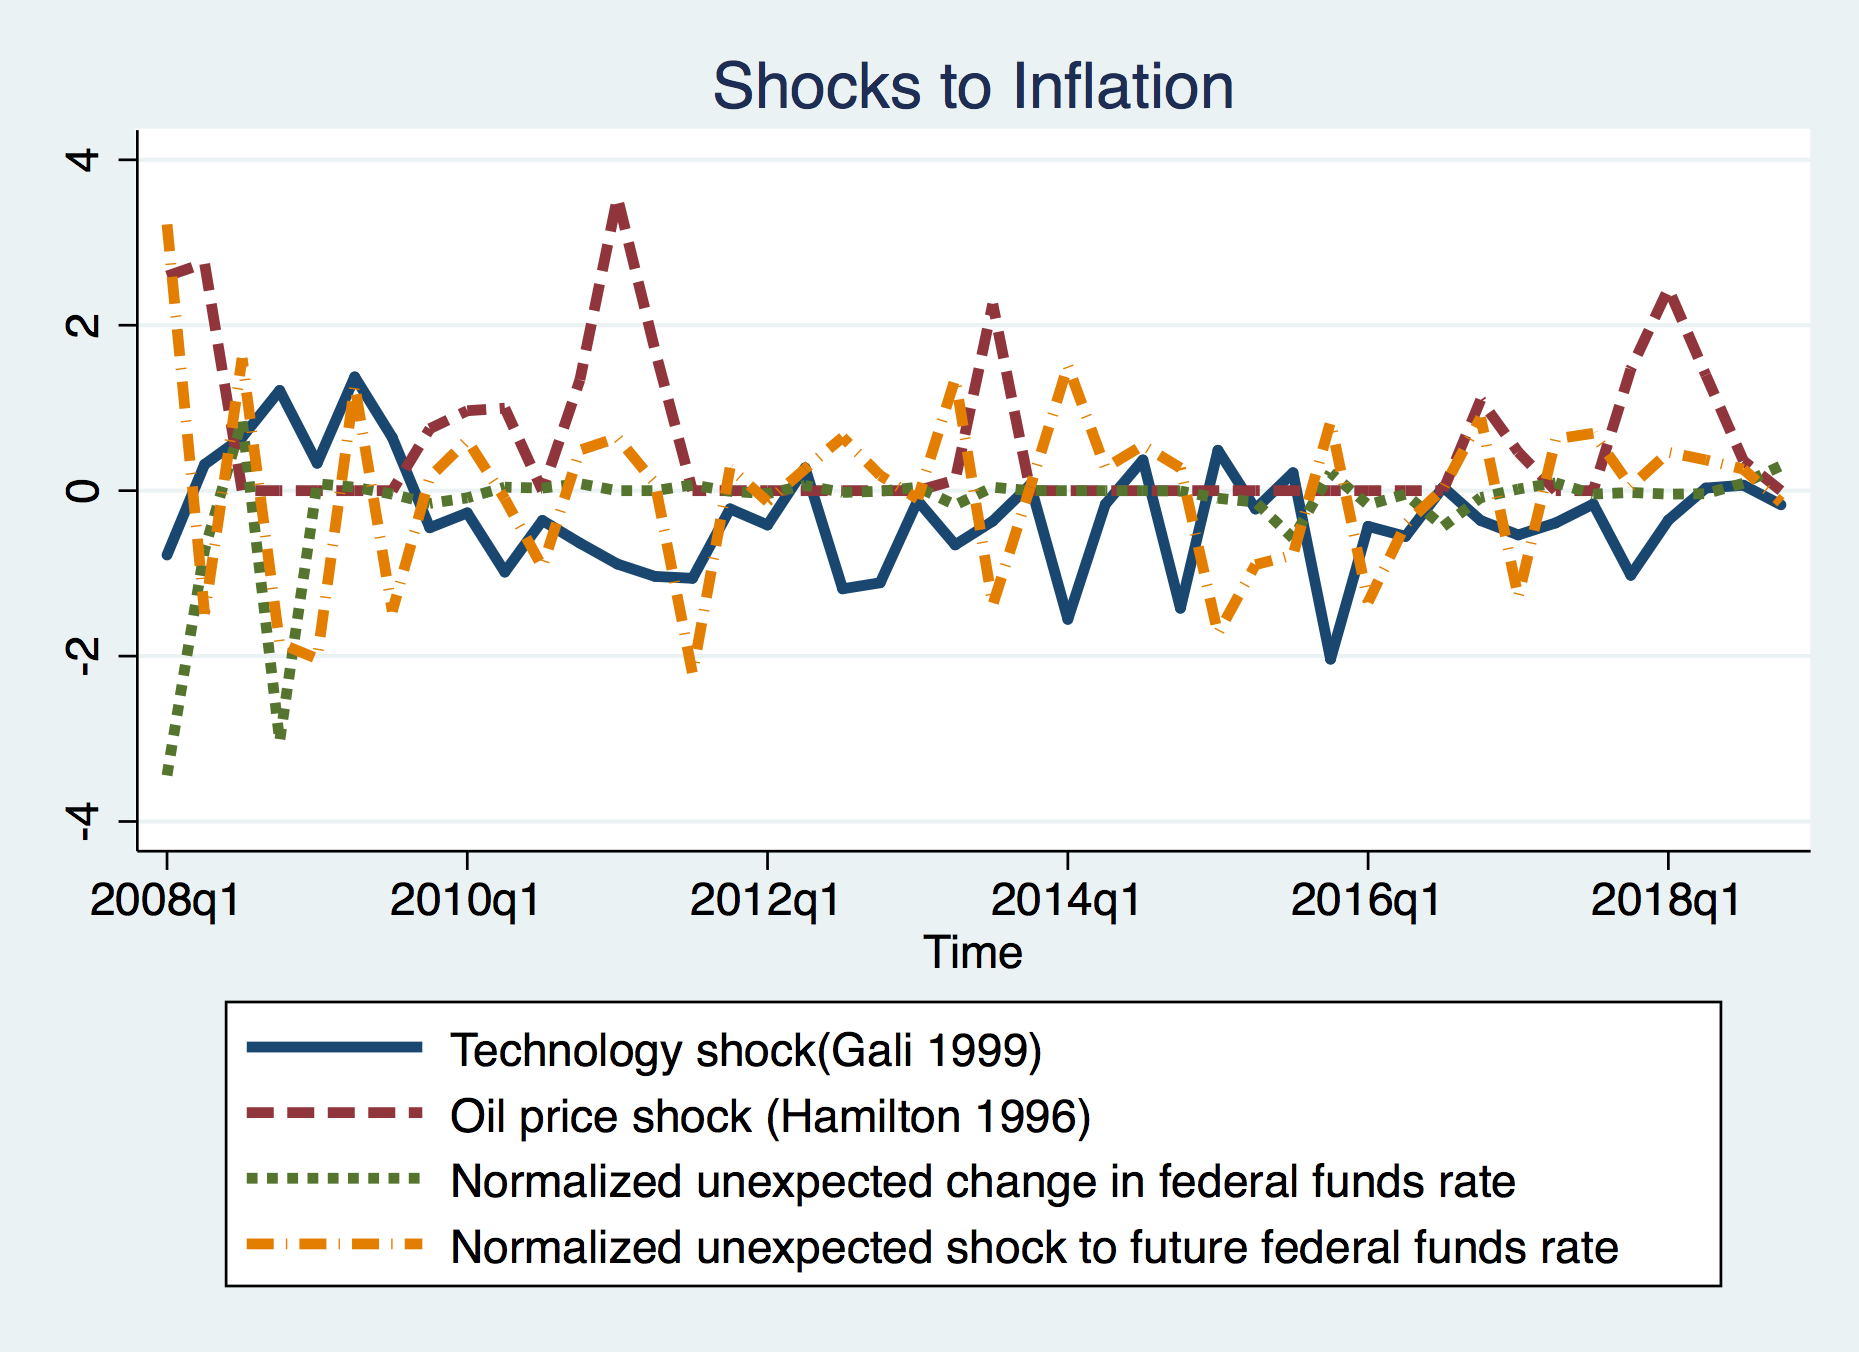
\includegraphics[width=0.8\textwidth]{figuresDraft/inf_shocksQ.png} 
\end{figure}

\end{frame}

\begin{frame}{Results from \cite{coibion2012can}}

\begin{figure}
	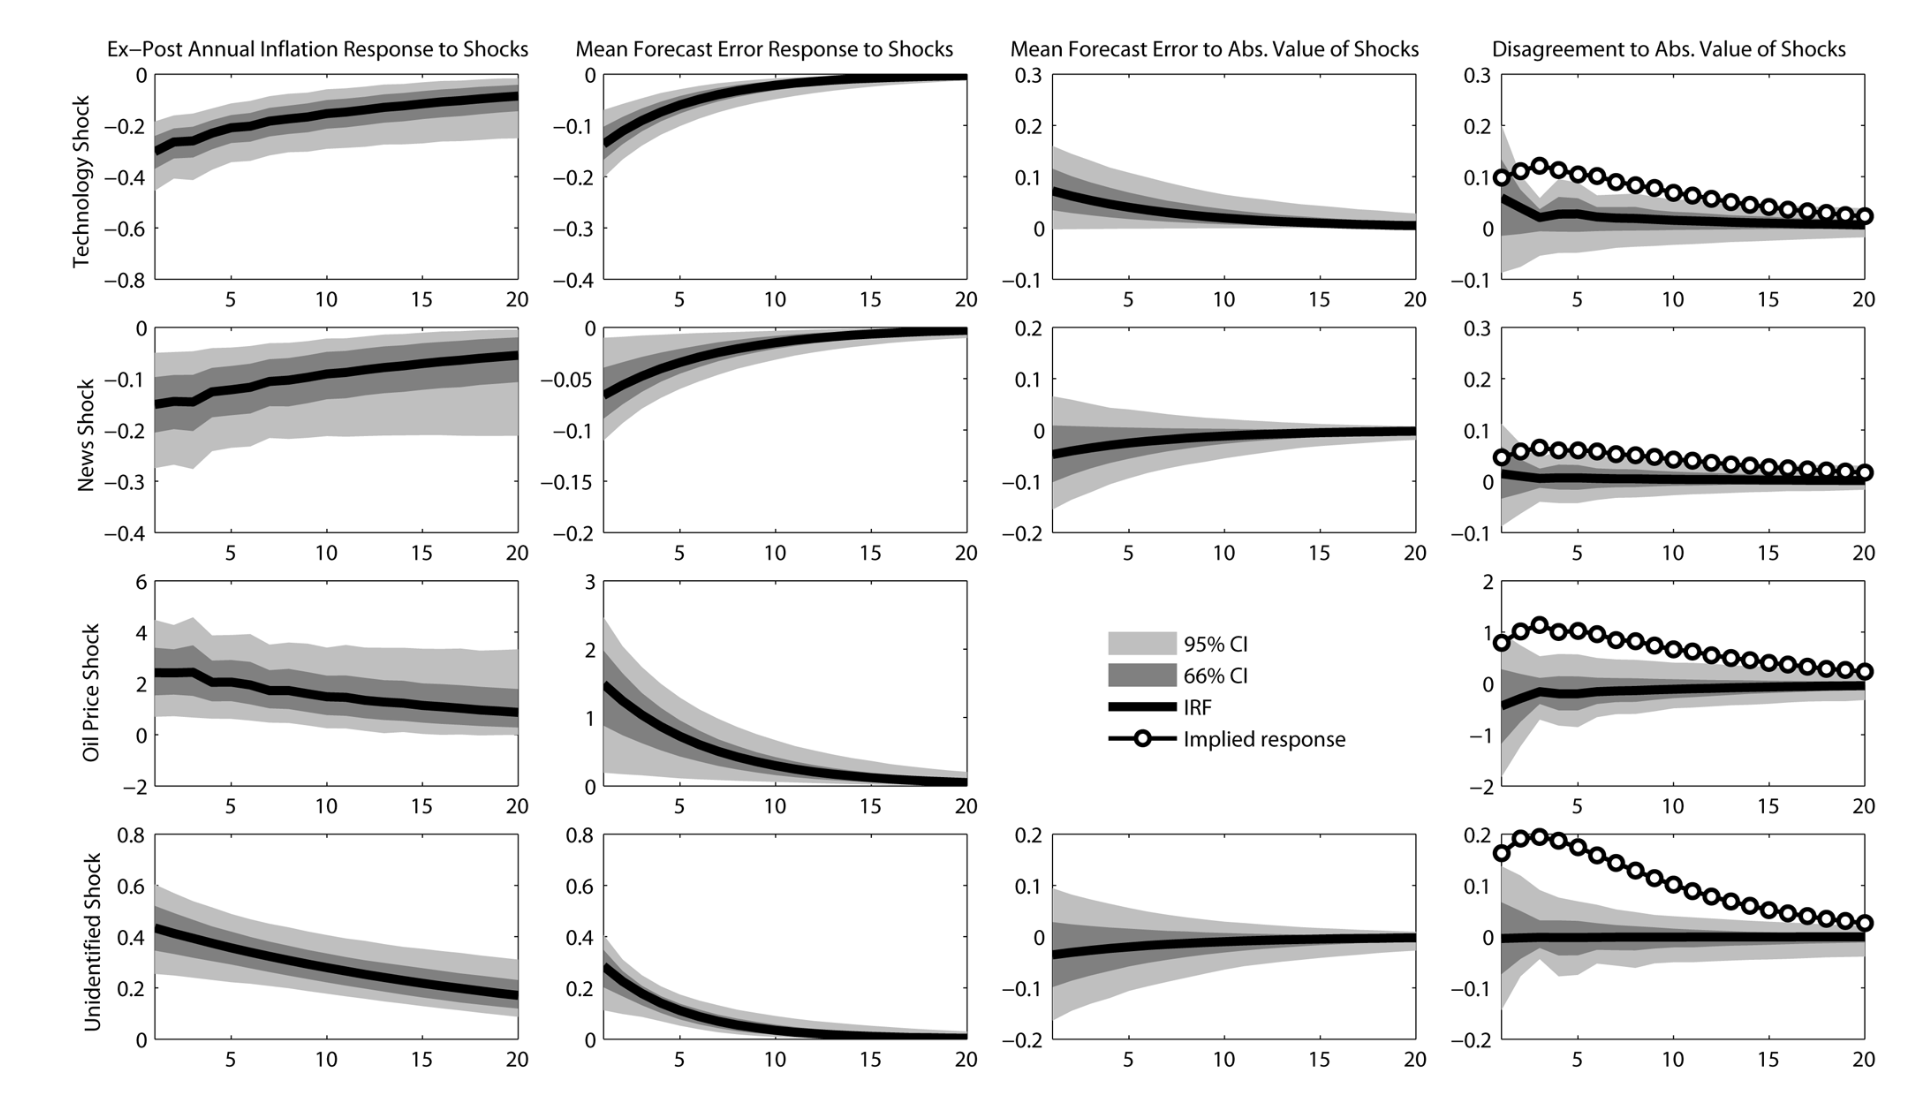
\includegraphics[width=0.9\textwidth]{figuresDraft/RigidityJPEFigure2.png} 
\end{figure}

\end{frame}

\begin{frame}{Technology and oil shocks: 1984-2007}

\begin{figure}
	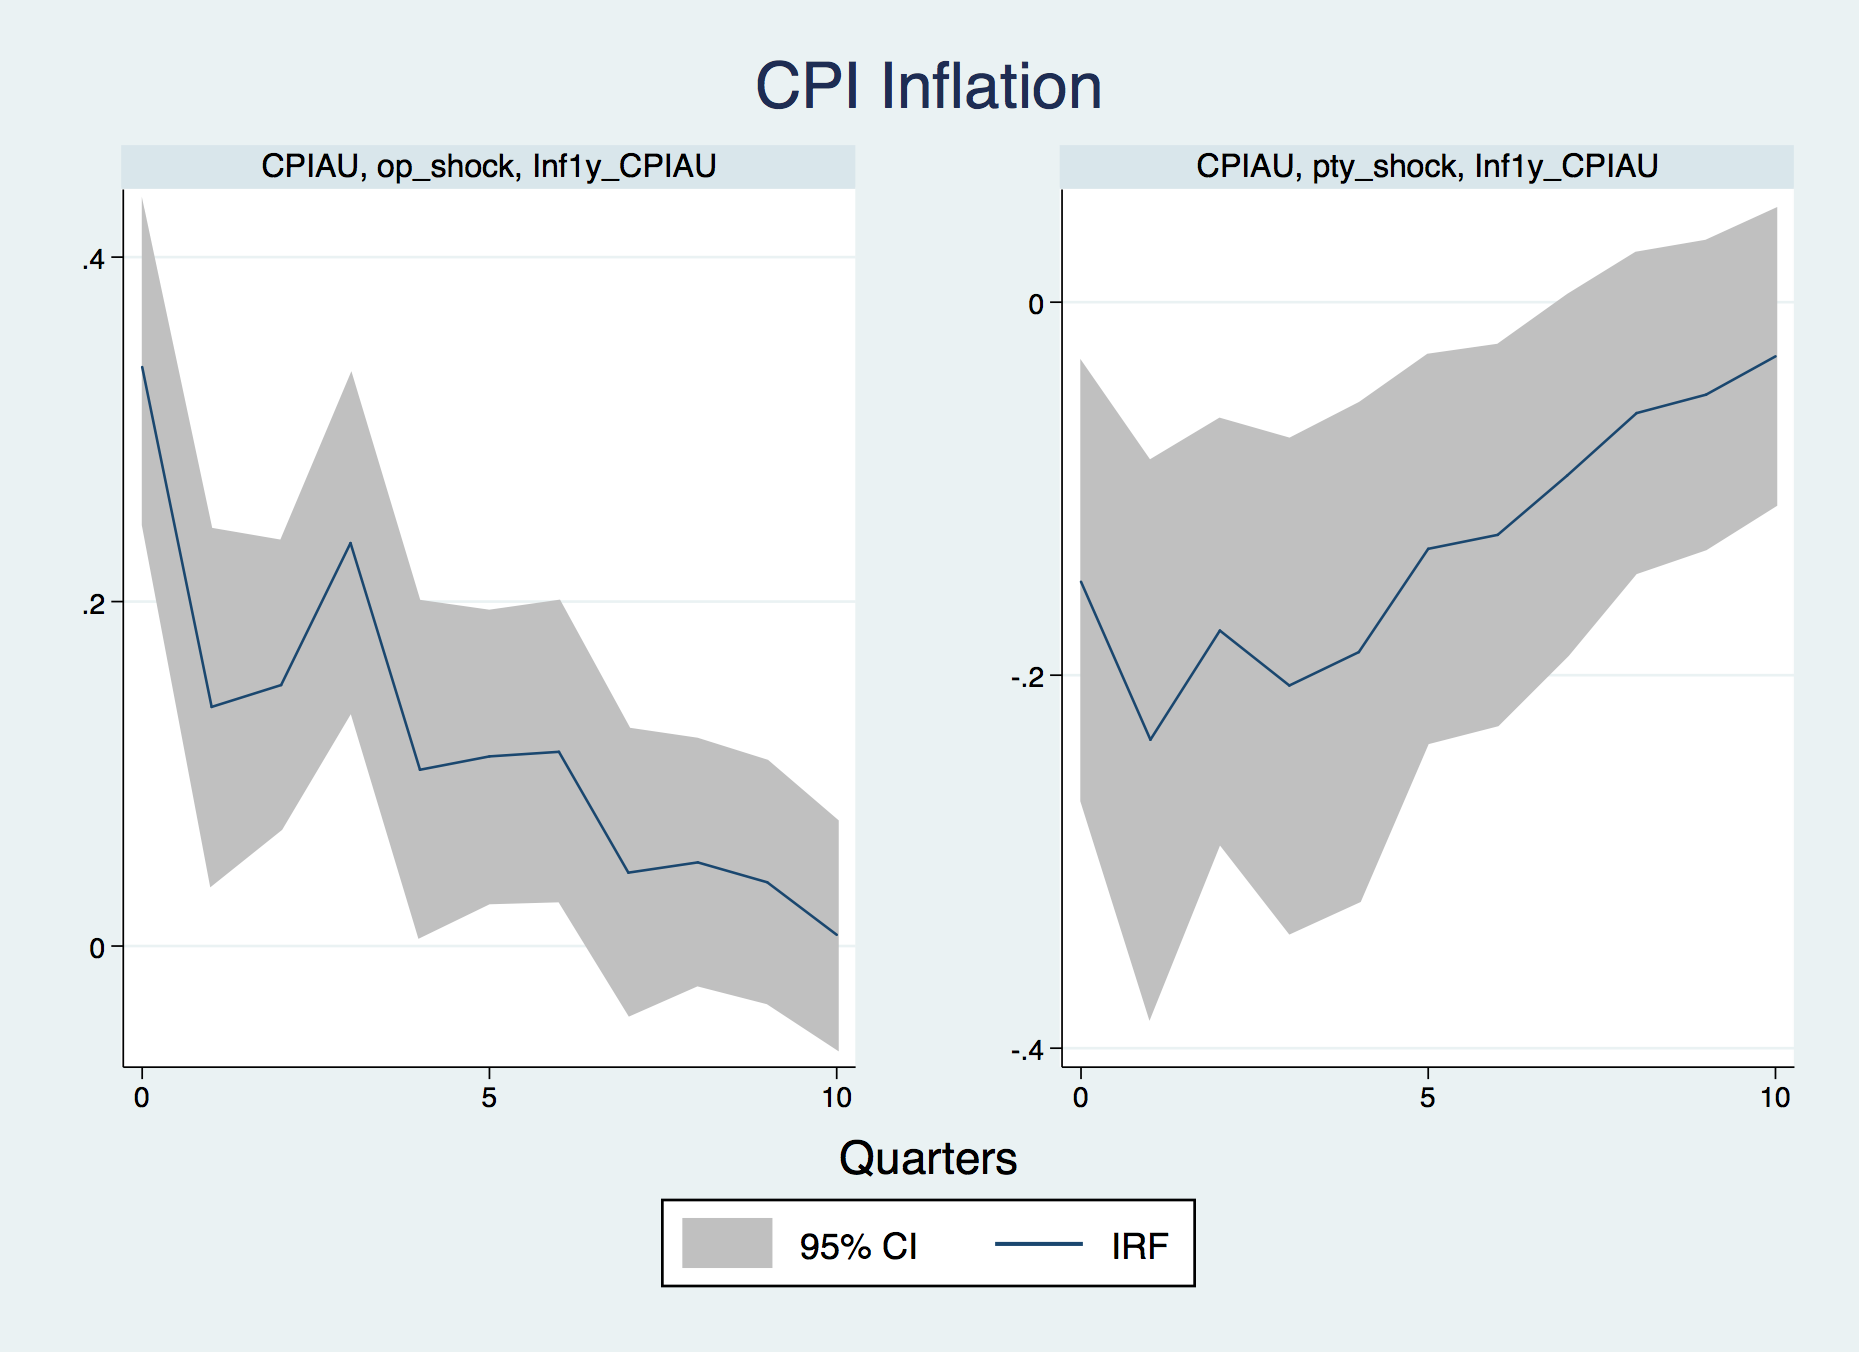
\includegraphics[width=0.5\textwidth,totalheight=0.28\textheight]{figuresDraft/CPIAU_ashocks_nmp_before2007.png}  \\ 
\smallskip
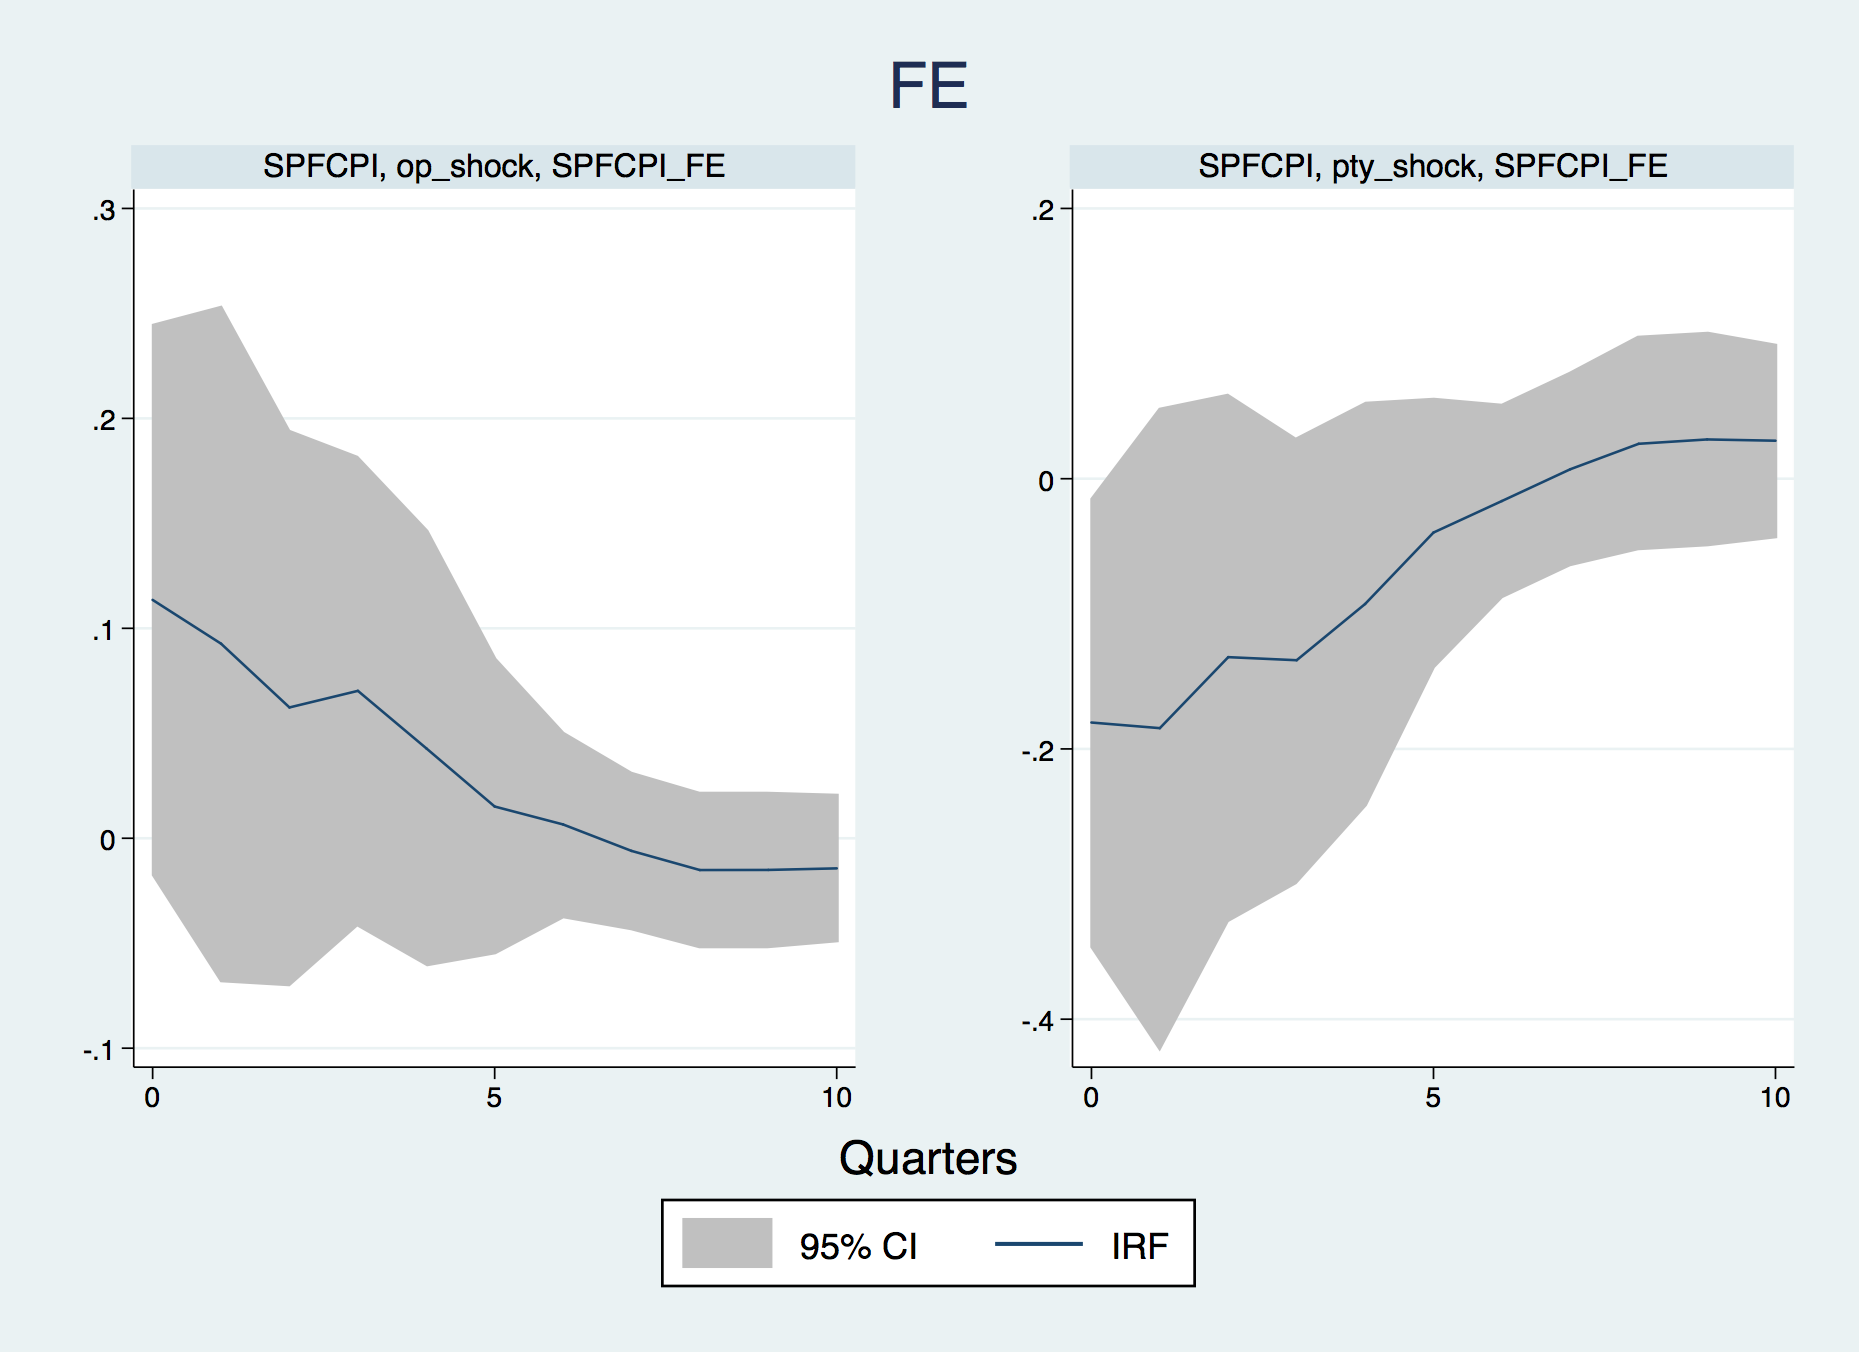
\includegraphics[width=0.5\textwidth,totalheight=0.28\textheight]{figuresDraft/SPFFE_ashocks_nmp_before2007.png} \\
\smallskip
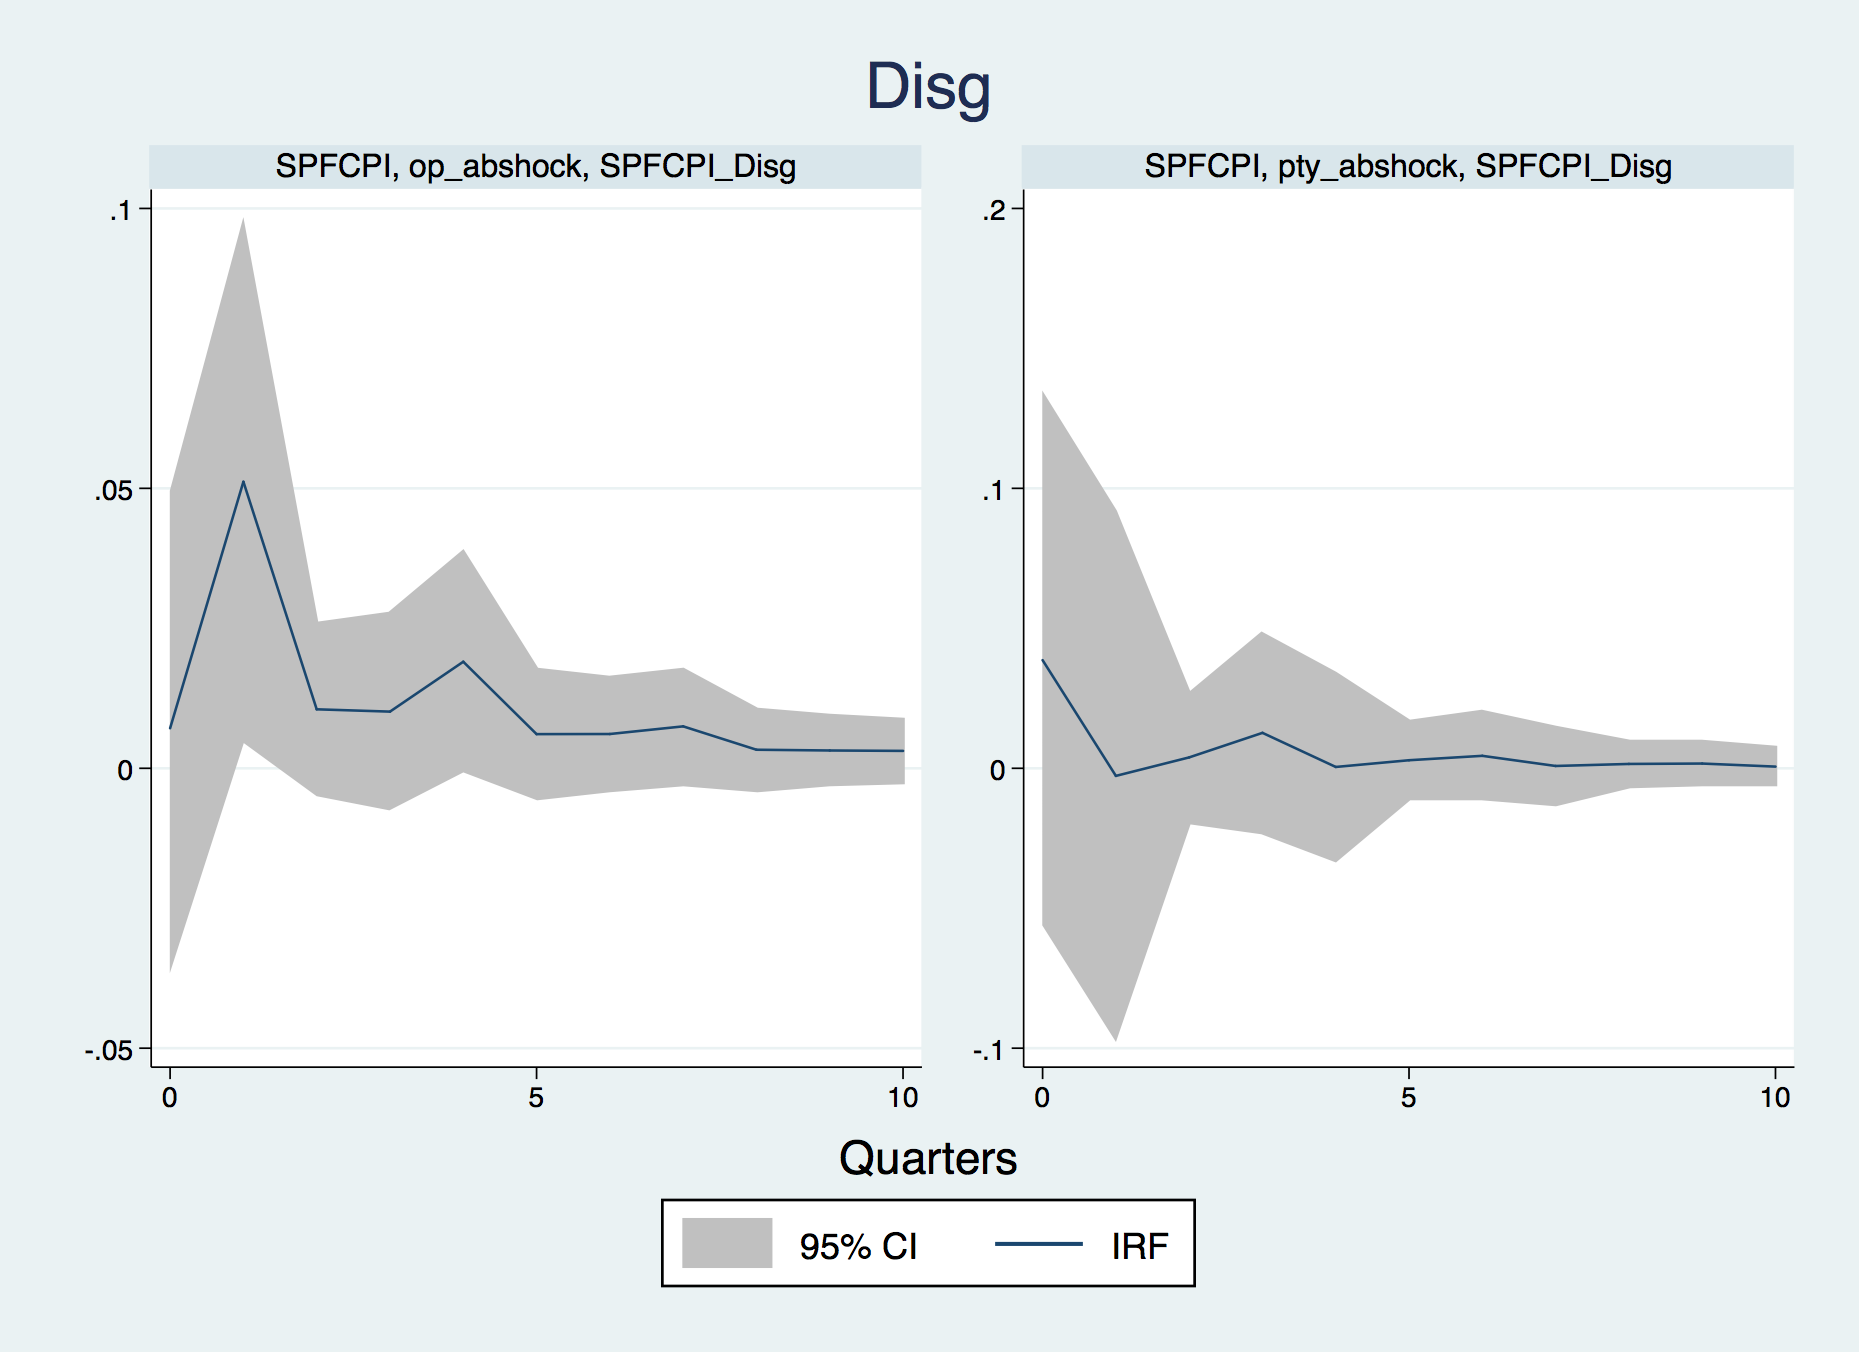
\includegraphics[width=0.5\textwidth,totalheight=0.28\textheight]{figuresDraft/SPFDisg_ab_ashocks_nmp_before2007.png} 
\end{figure}

\end{frame}


\begin{frame}{Monetary policy shocks: 1984-2007}

\begin{figure}
	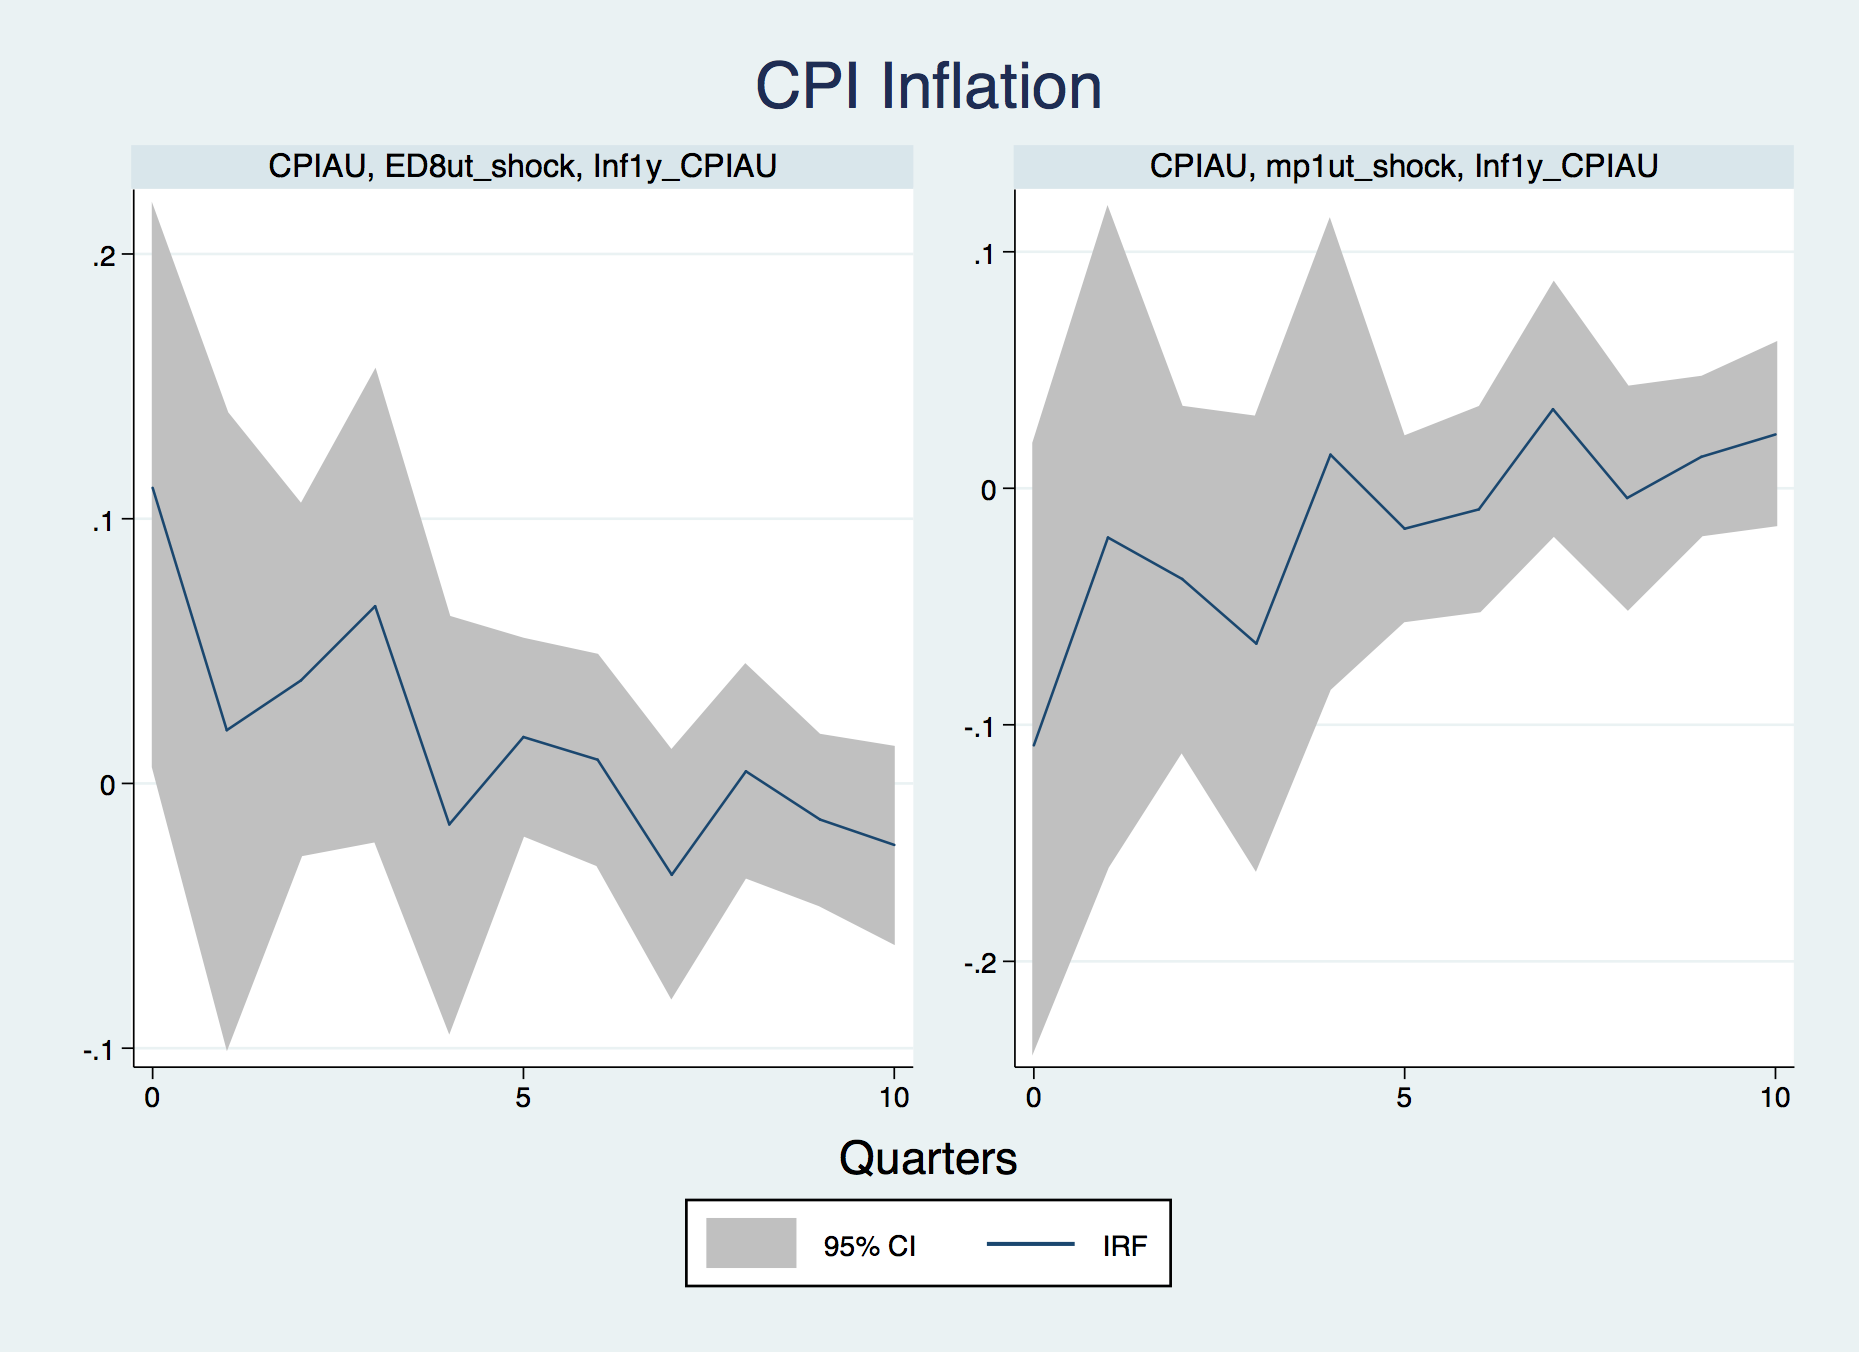
\includegraphics[width=0.5\textwidth,totalheight=0.28\textheight]{figuresDraft/CPIAU_ashocks_before2007.png}  \\
	\smallskip 
	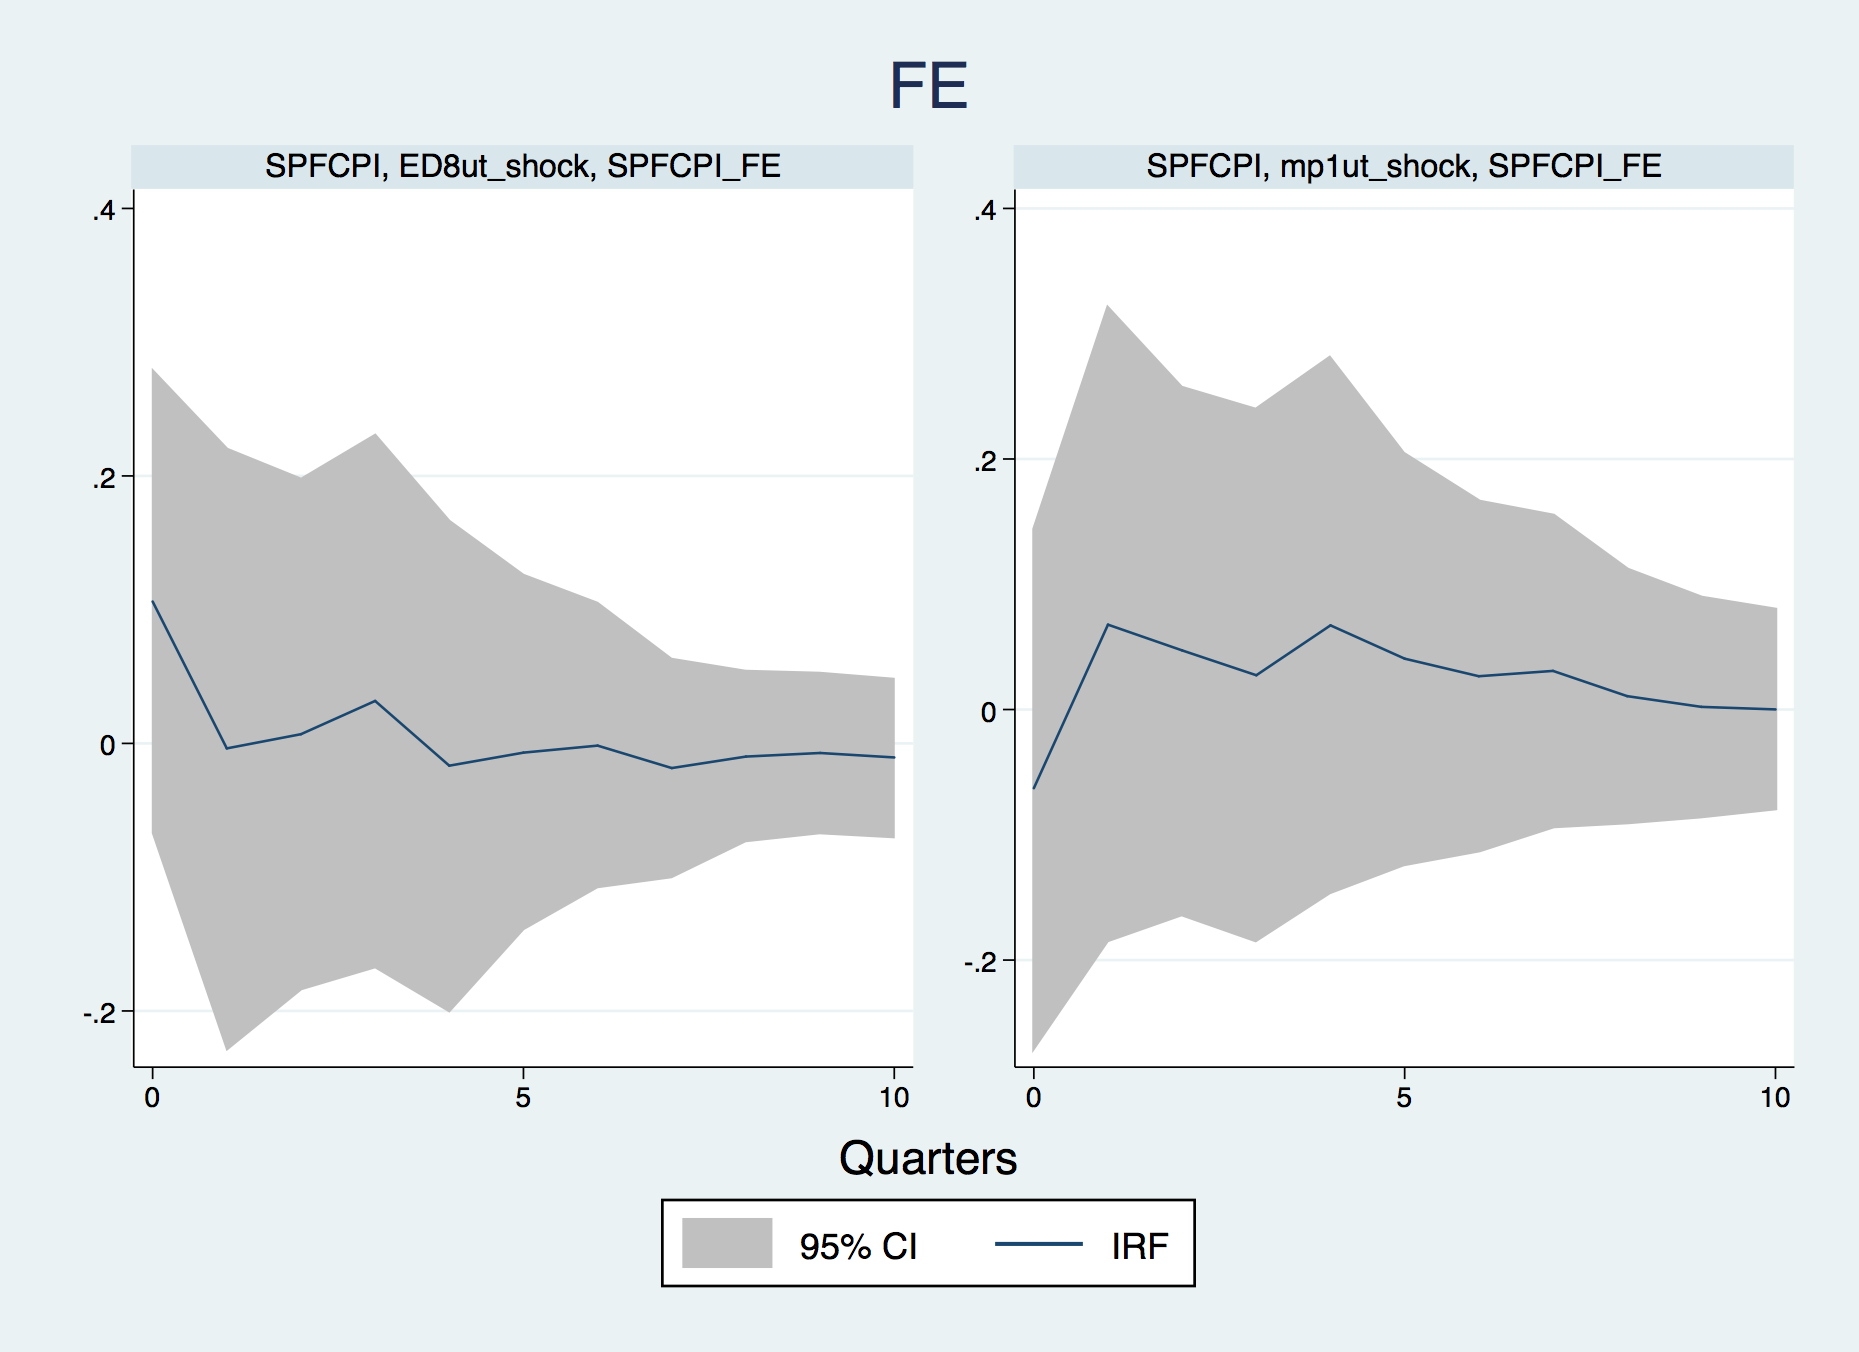
\includegraphics[width=0.5\textwidth,totalheight=0.28\textheight]{figuresDraft/SPFFE_ashocks_before2007.png} \\
	\smallskip
	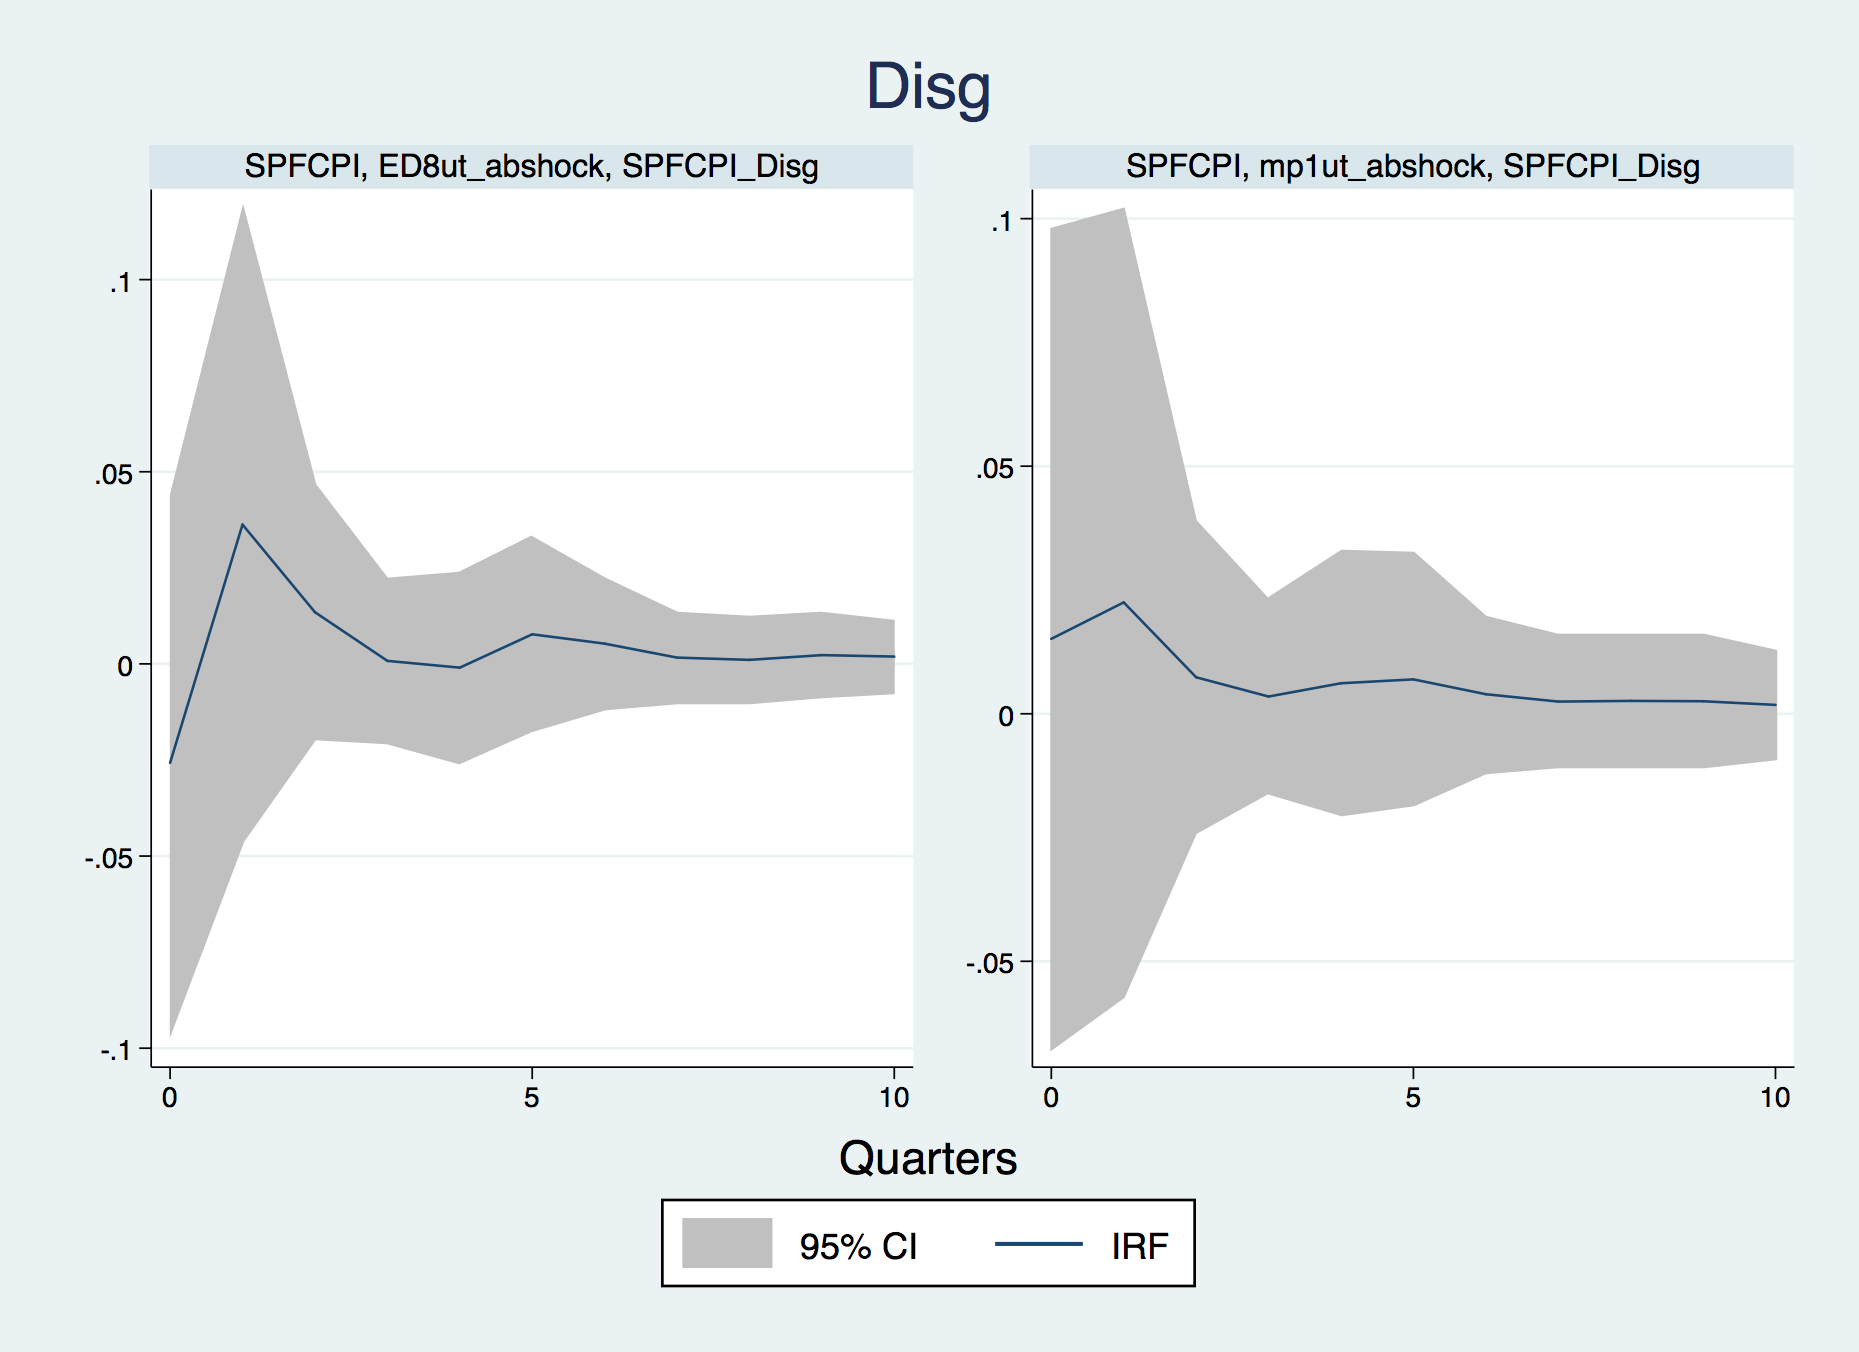
\includegraphics[width=0.5\textwidth,totalheight=0.28\textheight]{figuresDraft/SPFDisg_ab_ashocks_before2007.png} 
\end{figure}

\end{frame}


\begin{frame}{Technology and oil shocks: 1984-2019}

\begin{figure}
	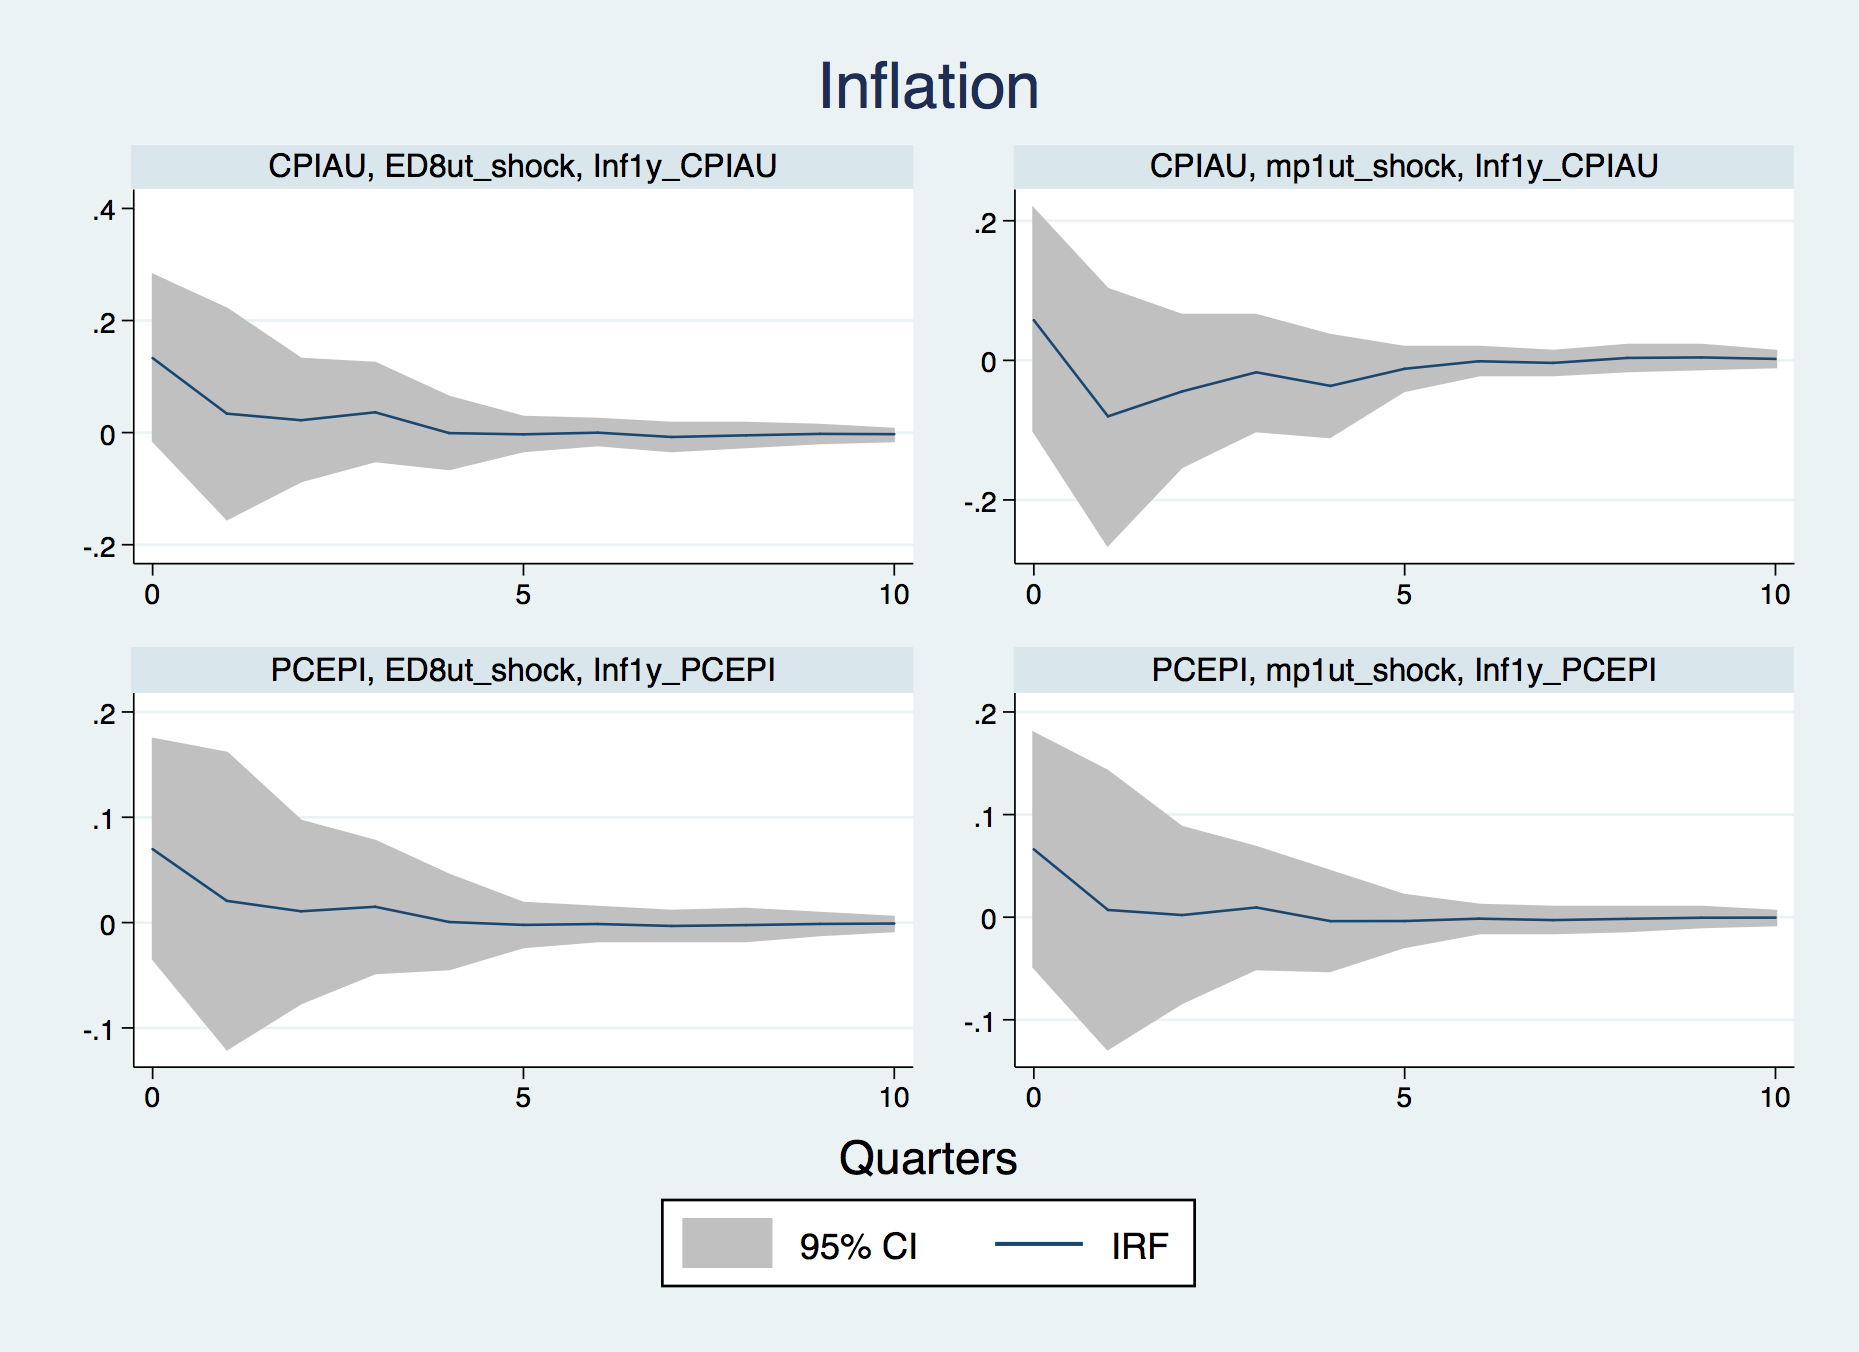
\includegraphics[width=7cm]{figuresDraft/Inf_ashocks.png} 
	\smallskip
	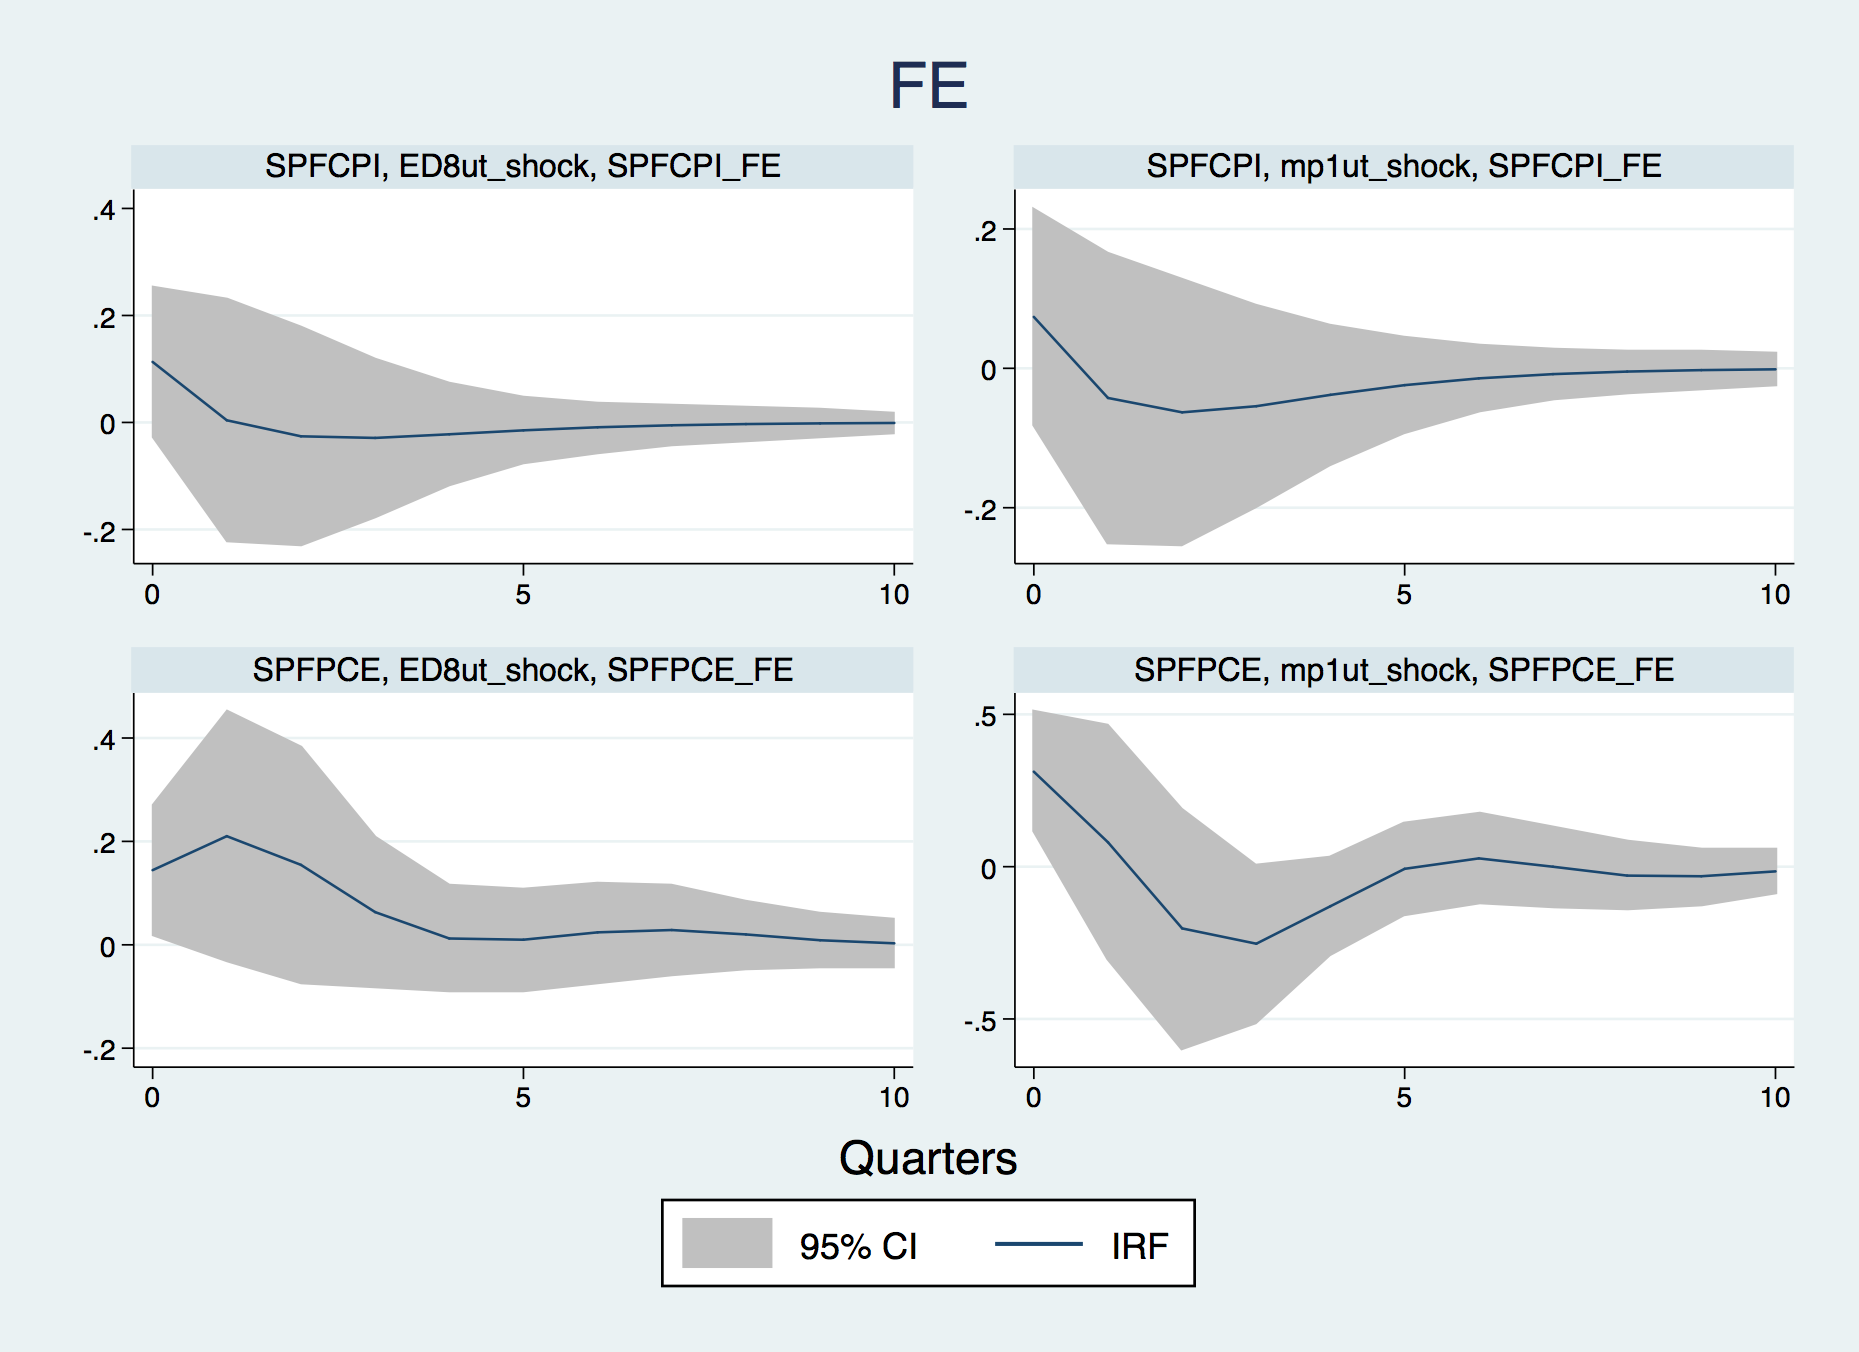
\includegraphics[width=7cm]{figuresDraft/SPFFE_ashocks.png} \\
	\smallskip
	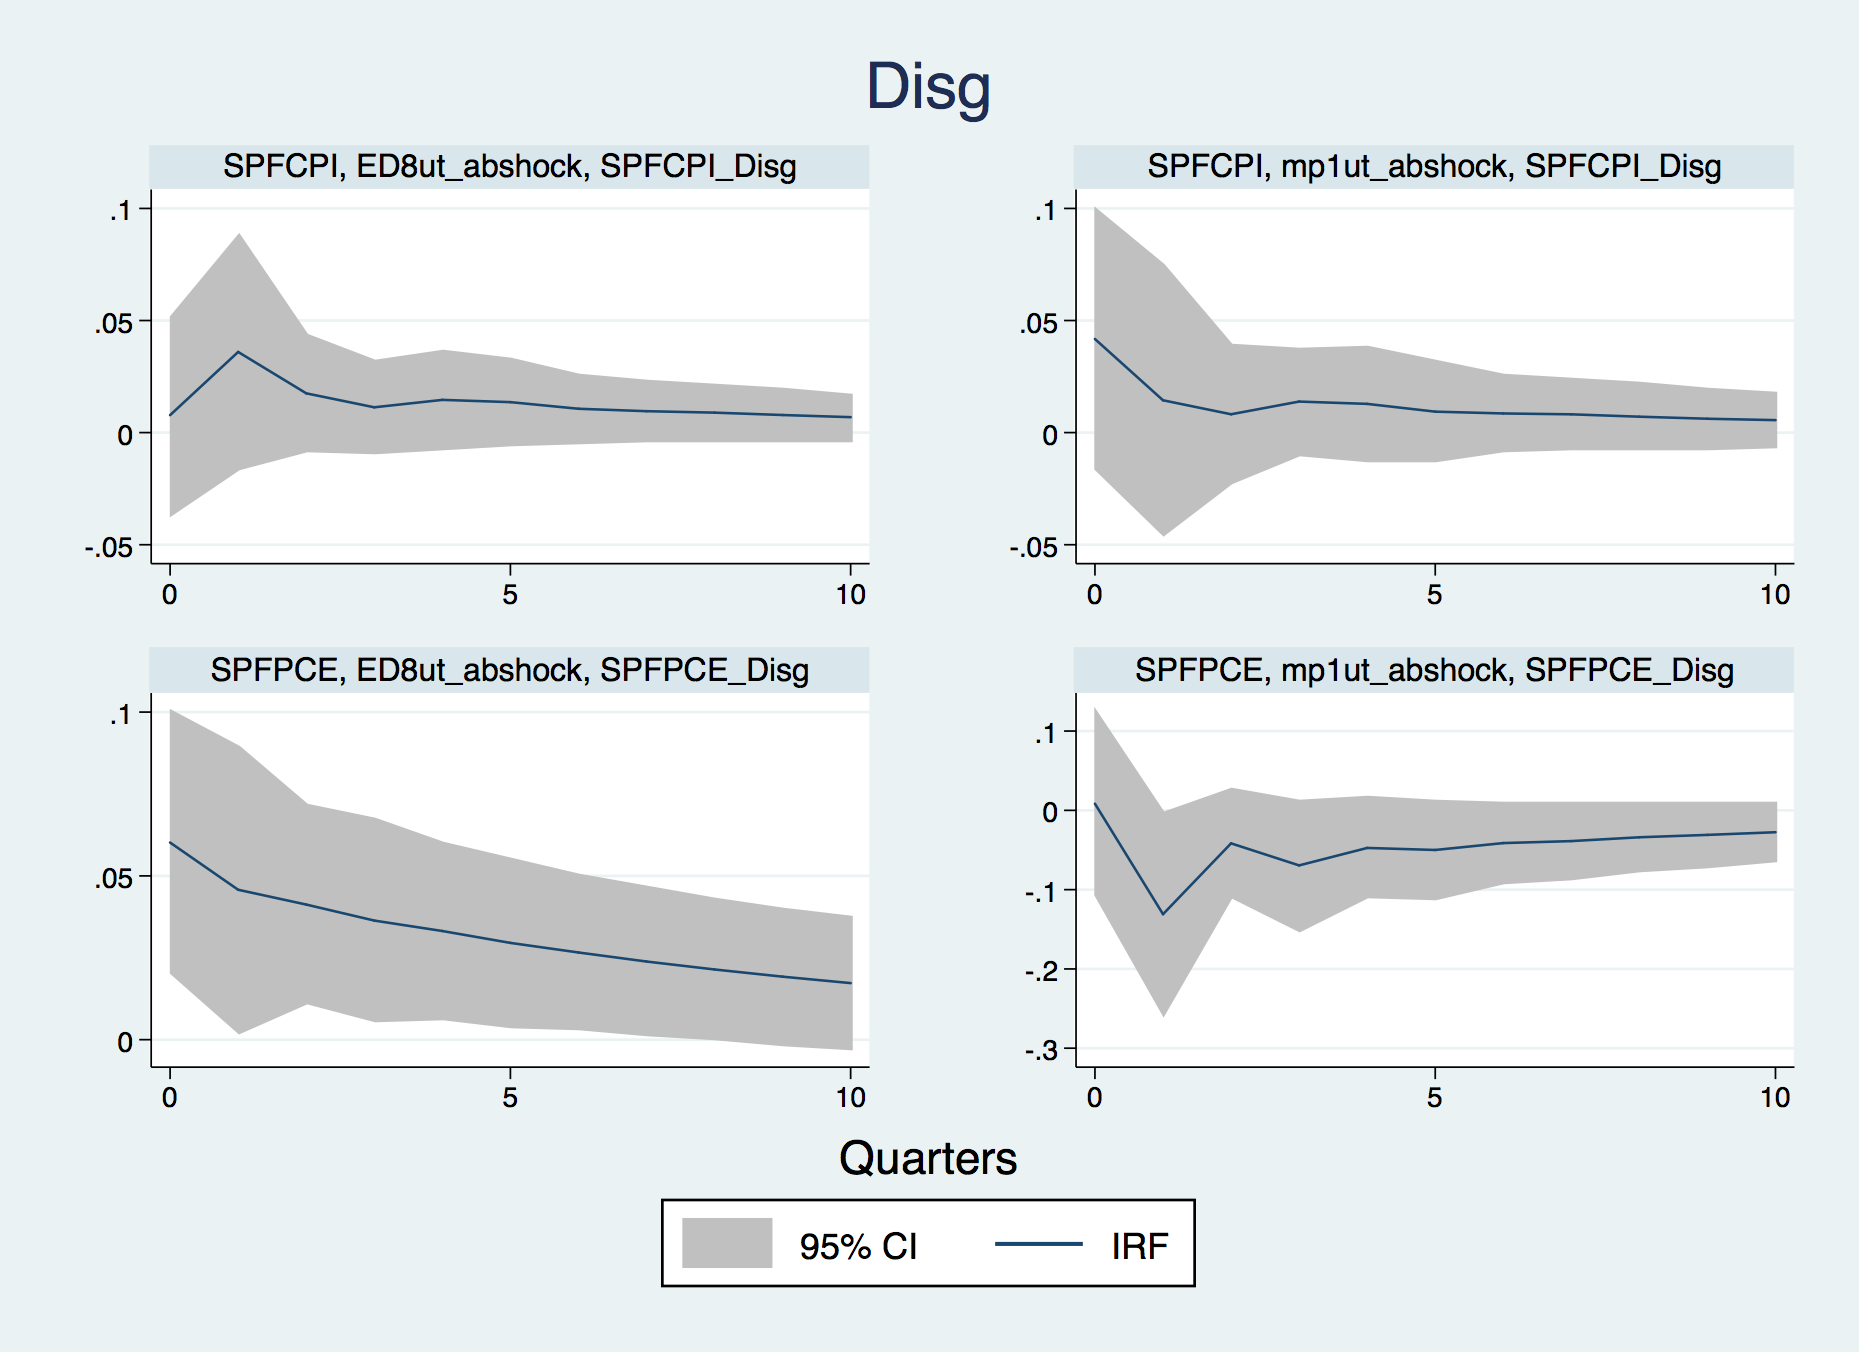
\includegraphics[width=7cm]{figuresDraft/SPFDisg_ab_ashocks.png} 
	\smallskip
	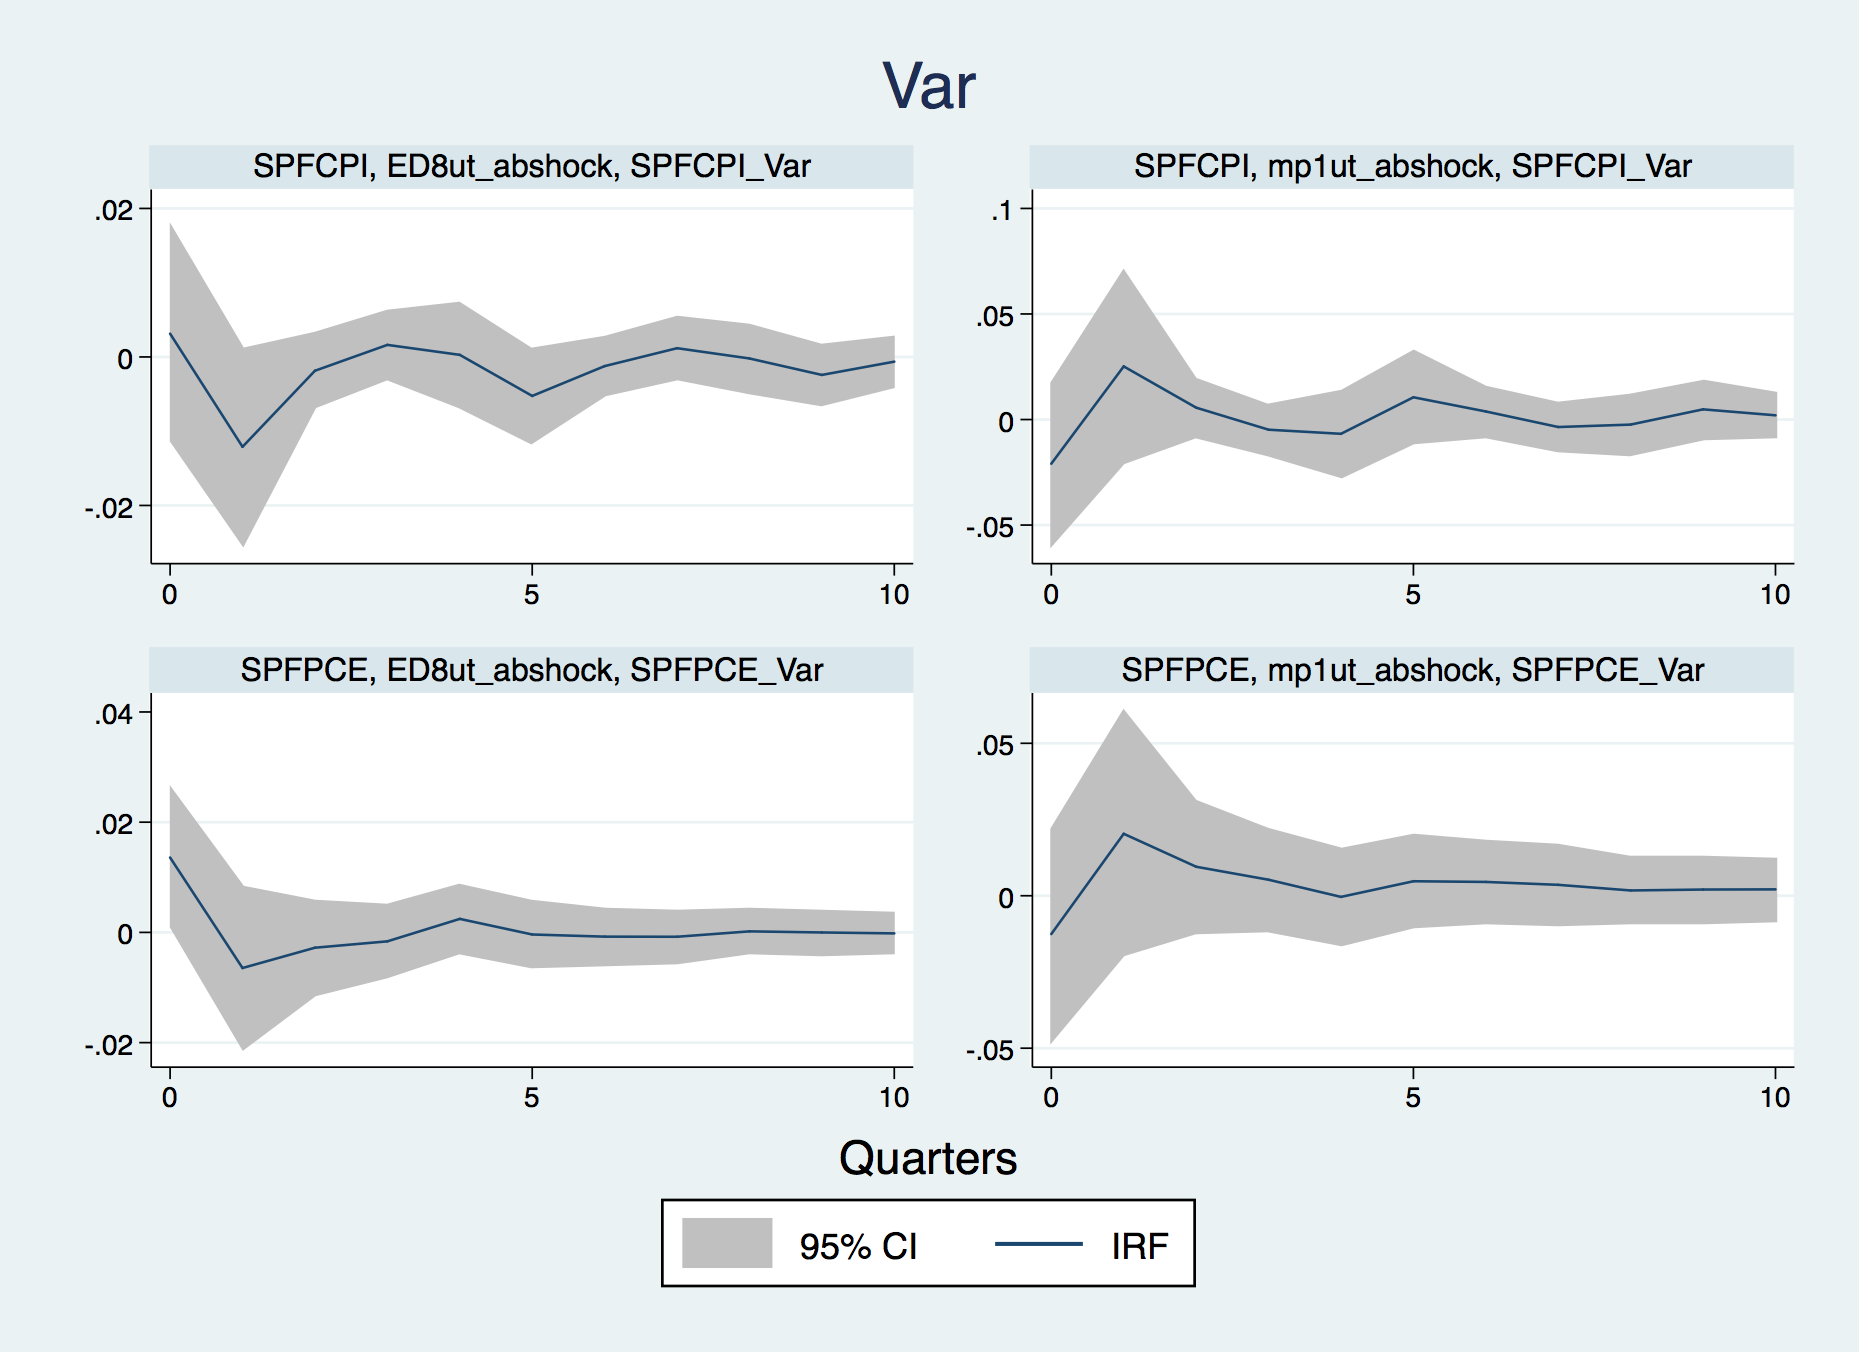
\includegraphics[width=7cm]{figuresDraft/SPFVar_ab_ashocks.png}  
\end{figure}

\end{frame}


\begin{frame}{Monetary policy shocks: 1984-2019}

\begin{figure}
	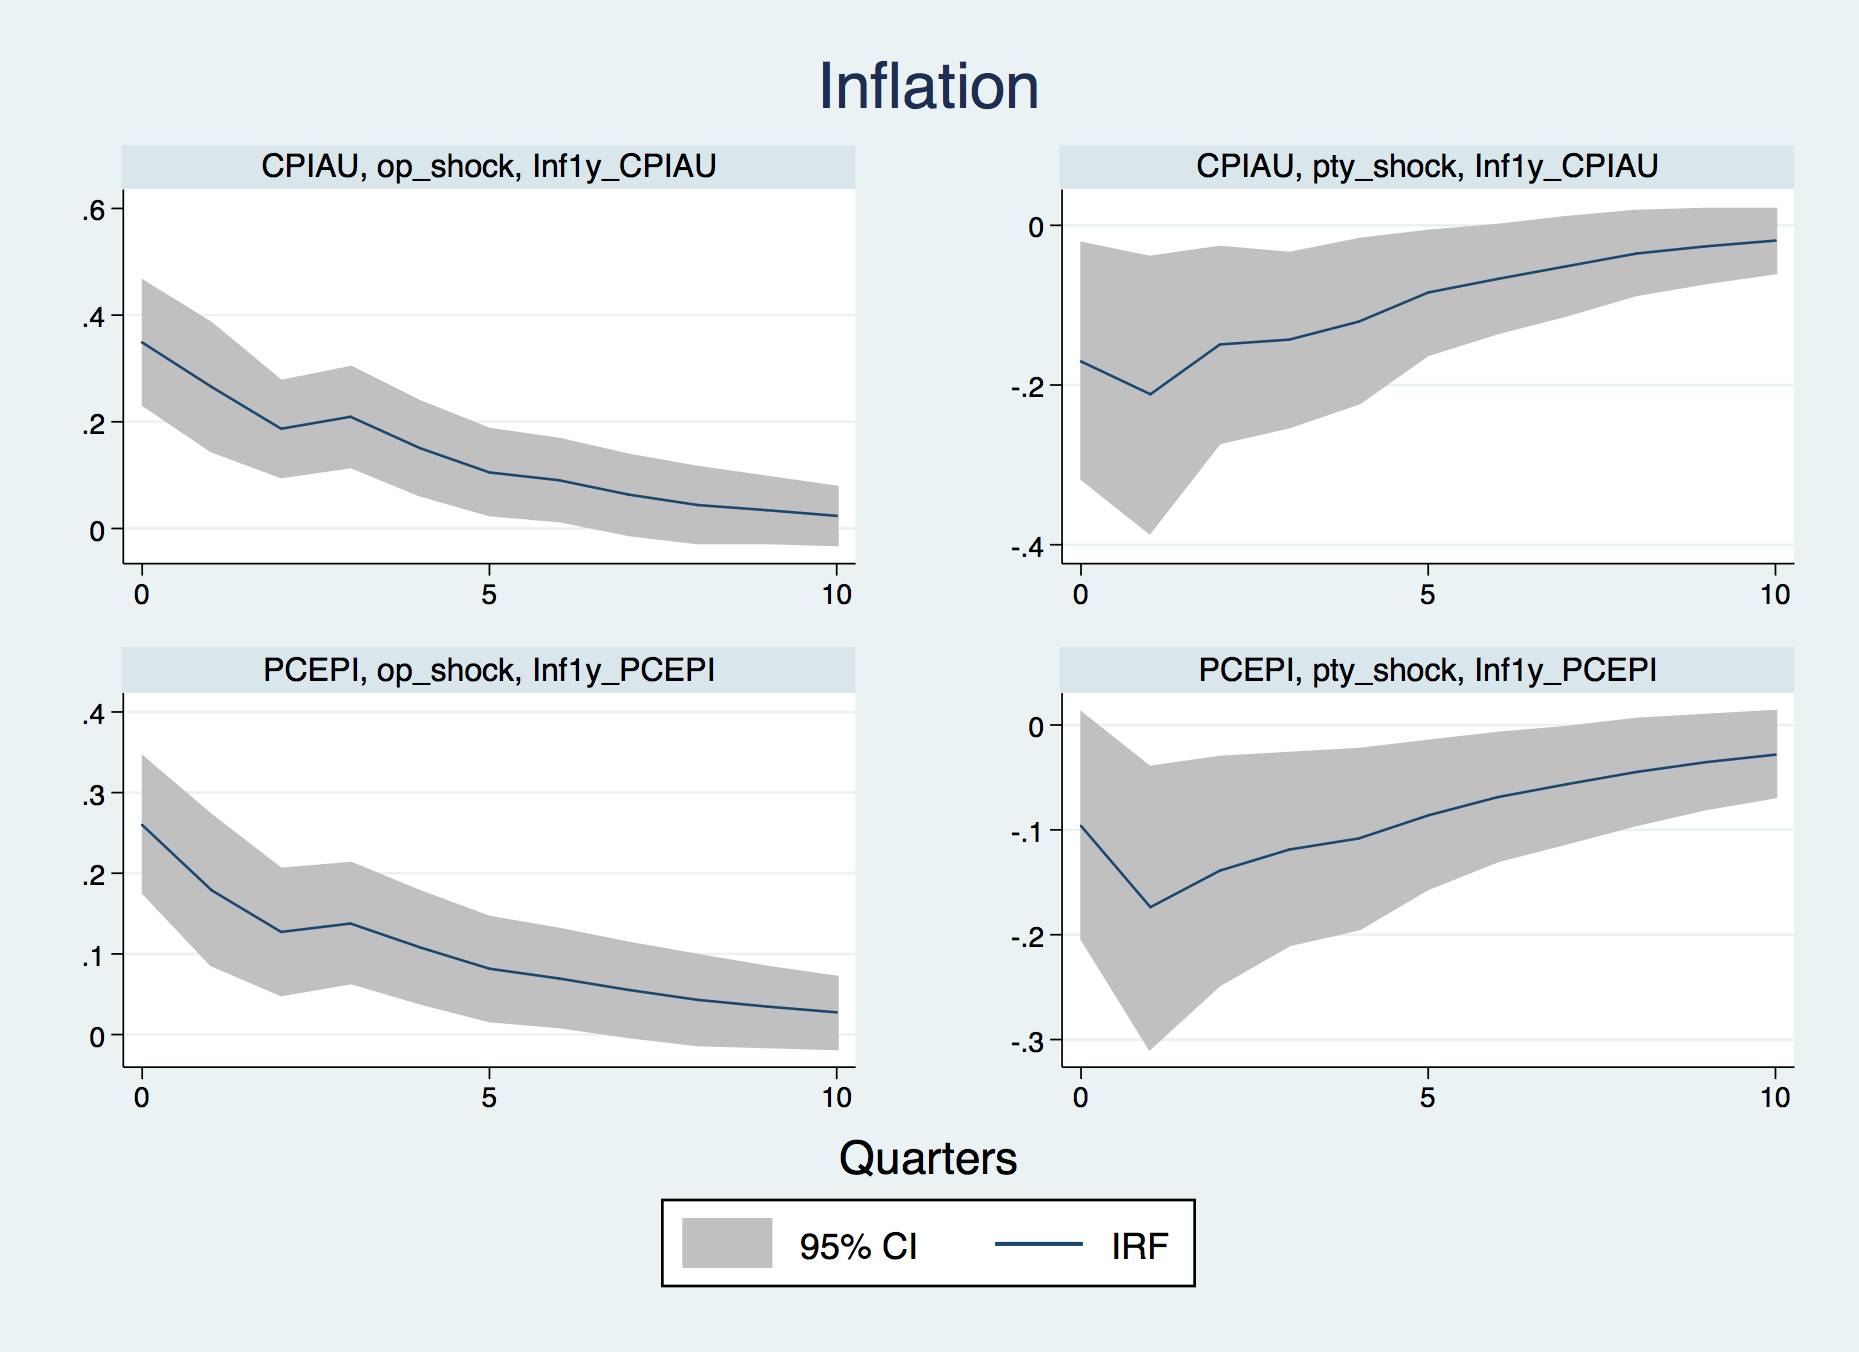
\includegraphics[width=7cm]{figuresDraft/Inf_ashocks_nmp.png}  
	
	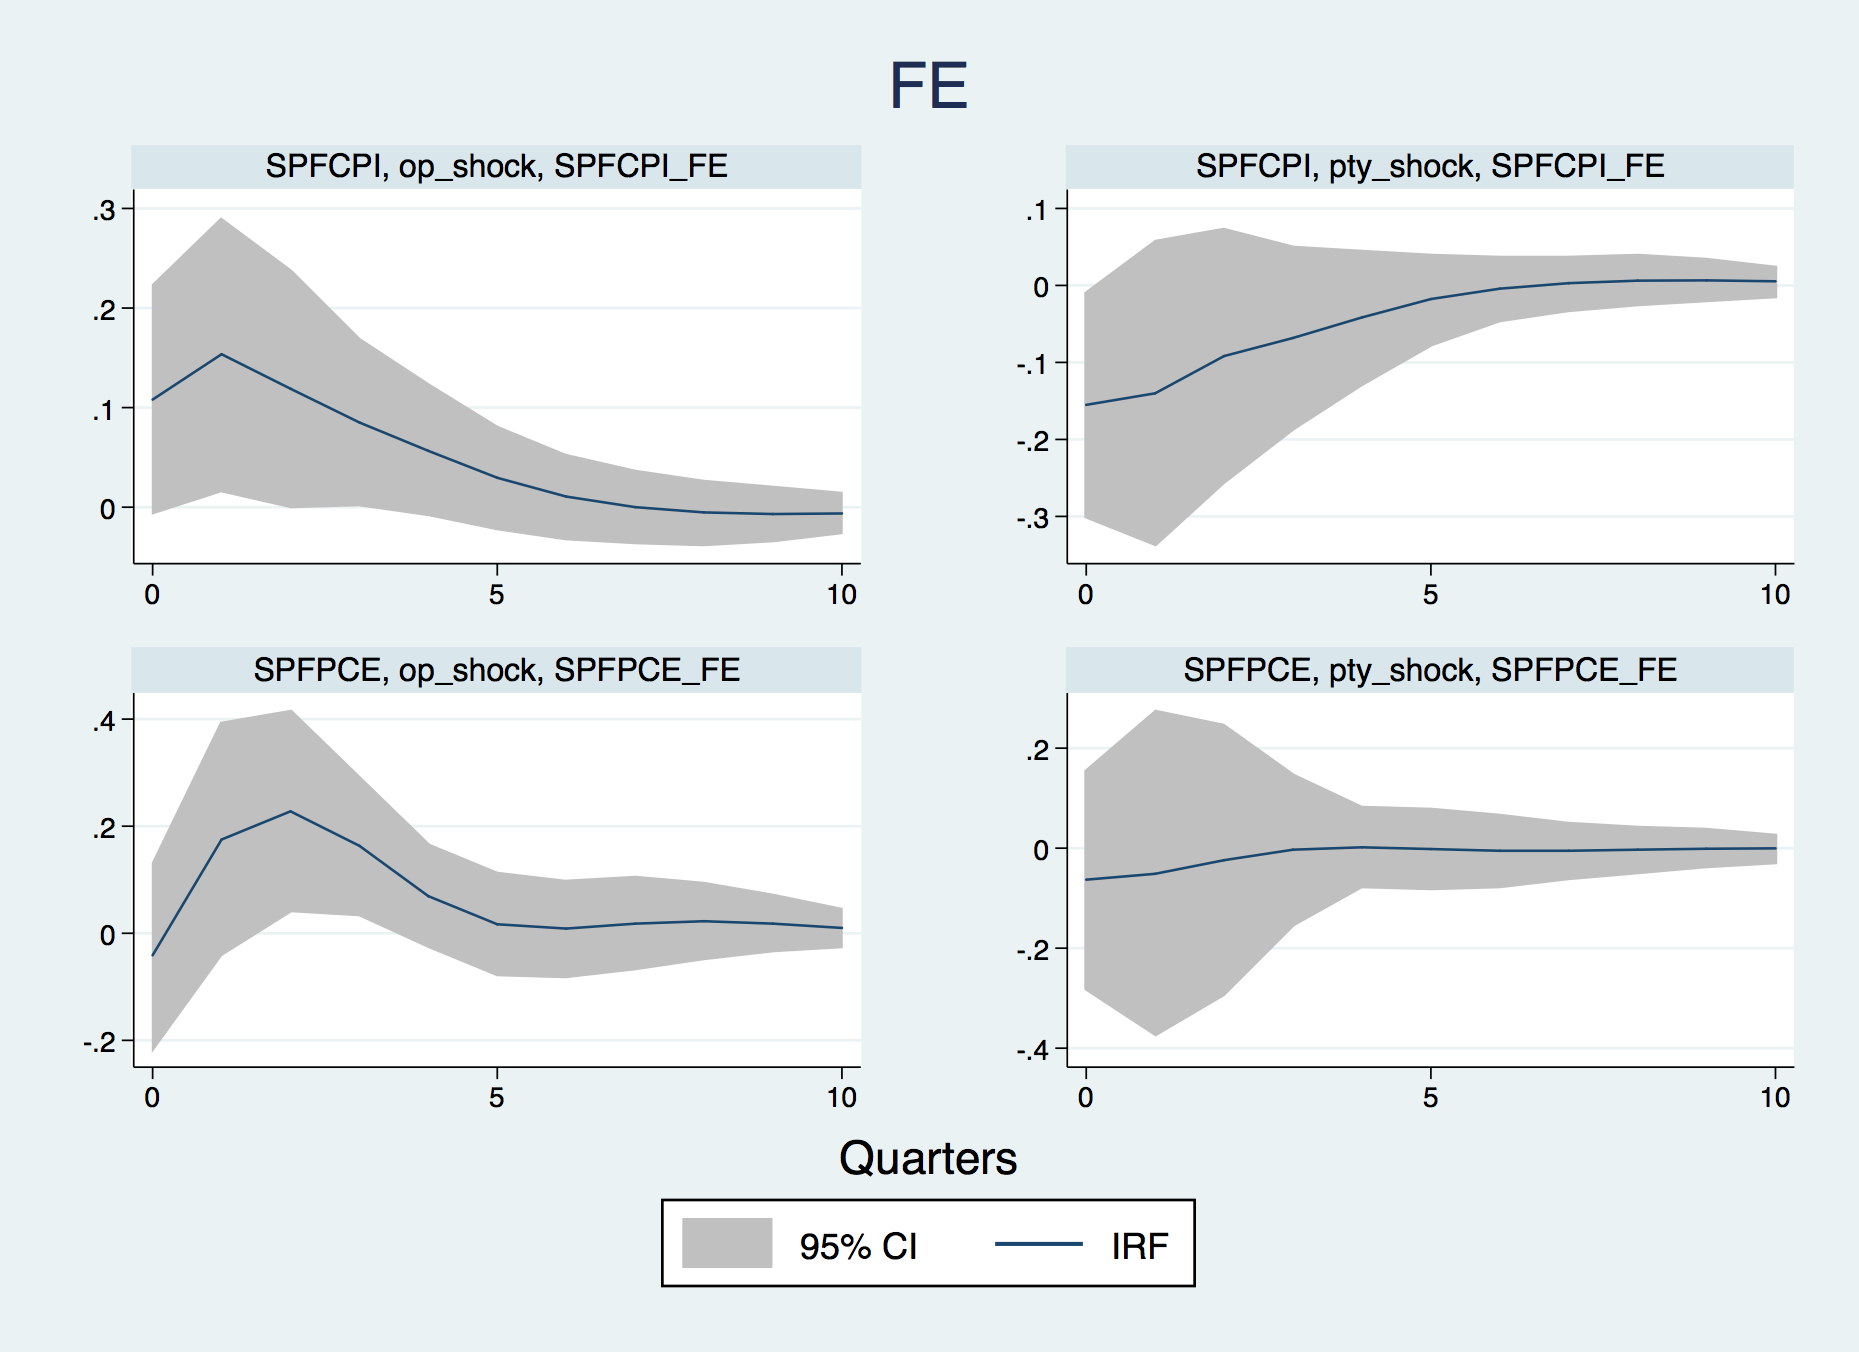
\includegraphics[width=7cm]{figuresDraft/SPFFE_ashocks_nmp.png}  \\
	\smallskip 
	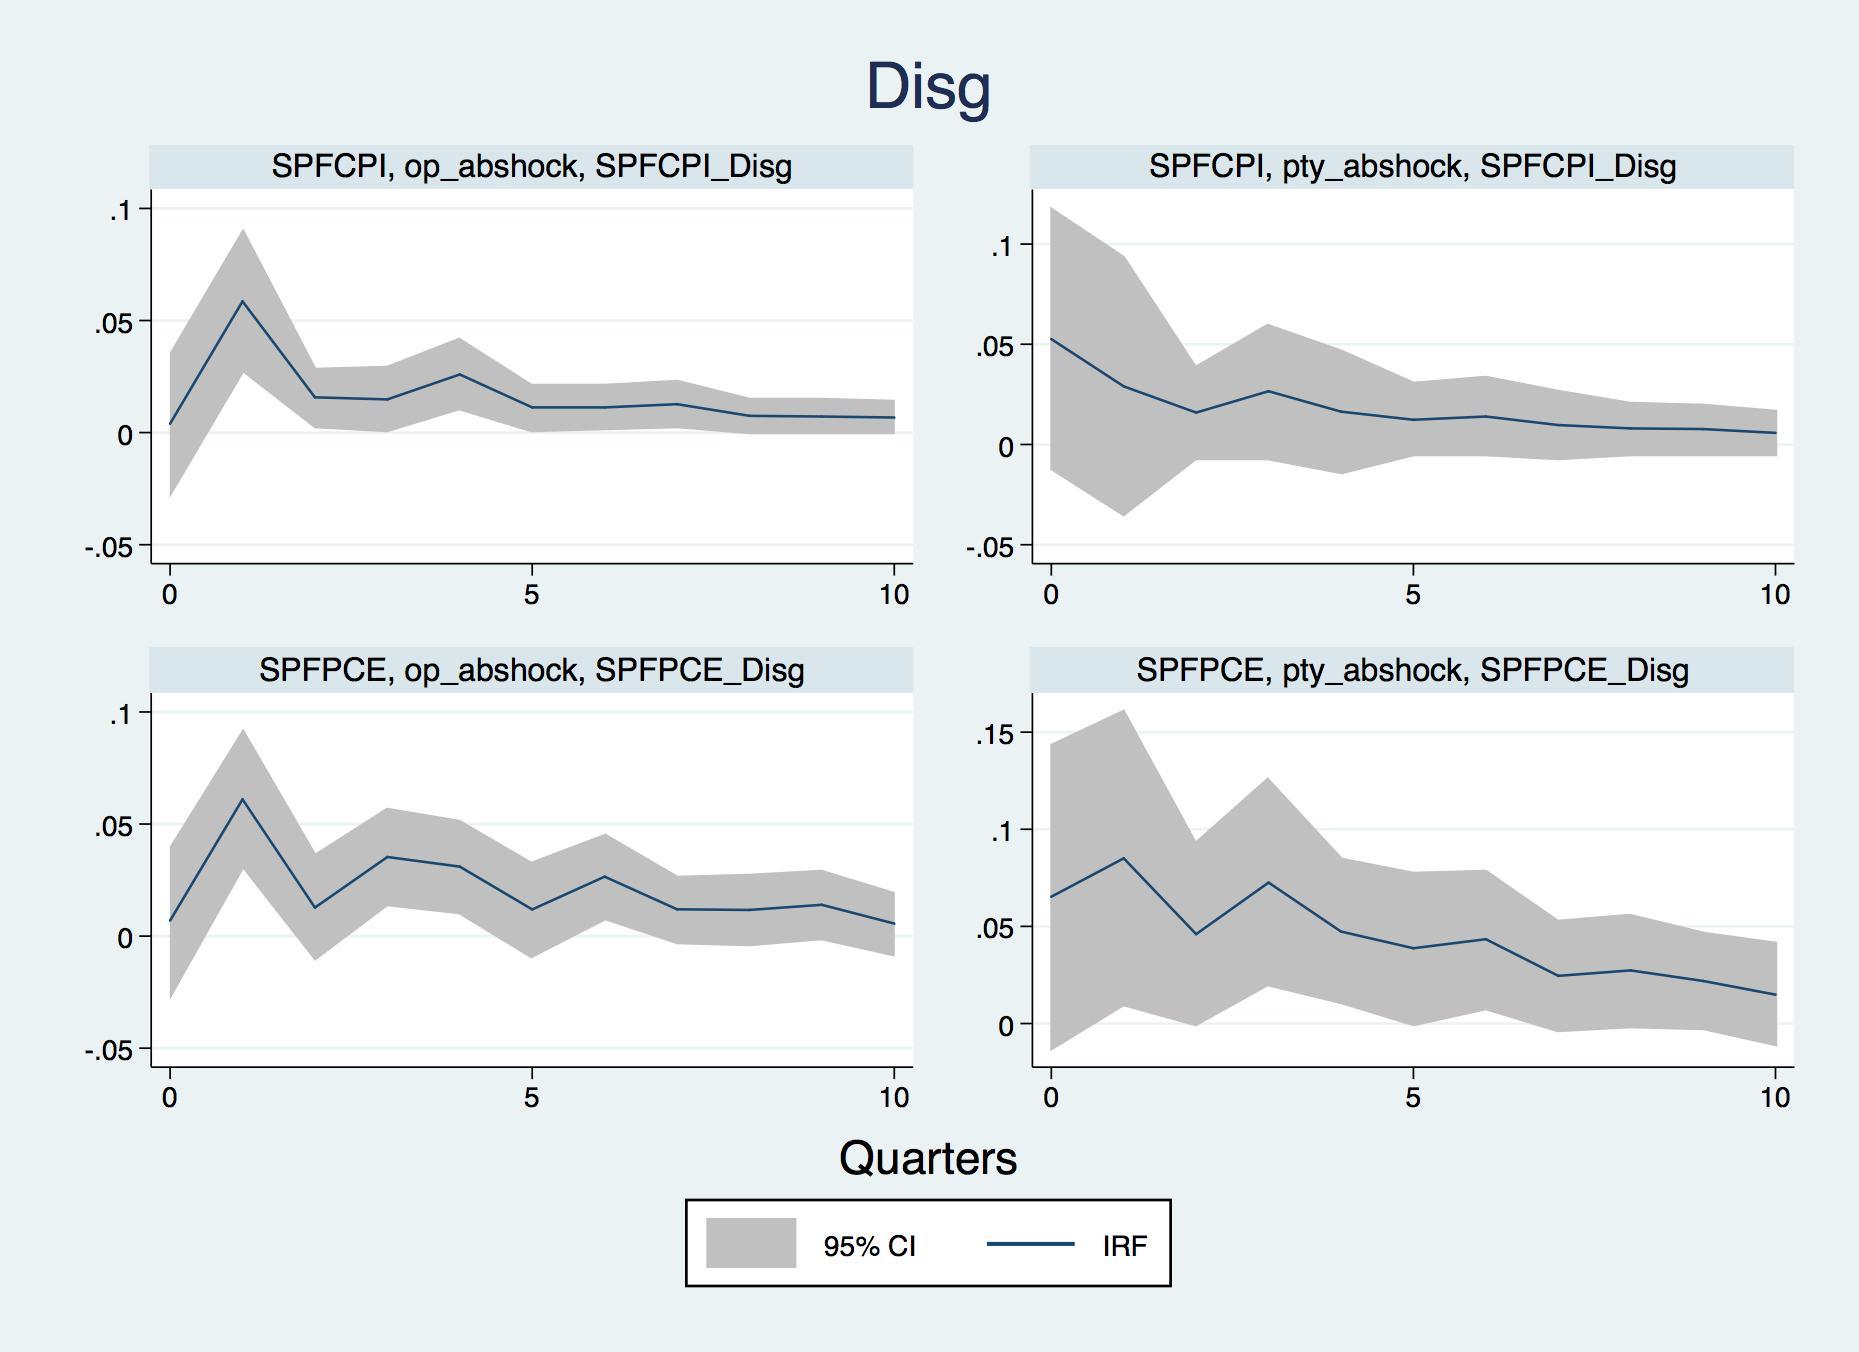
\includegraphics[width=7cm]{figuresDratf/SPFDisg_ab_ashocks_nmp.png} 
	\smallskip 
	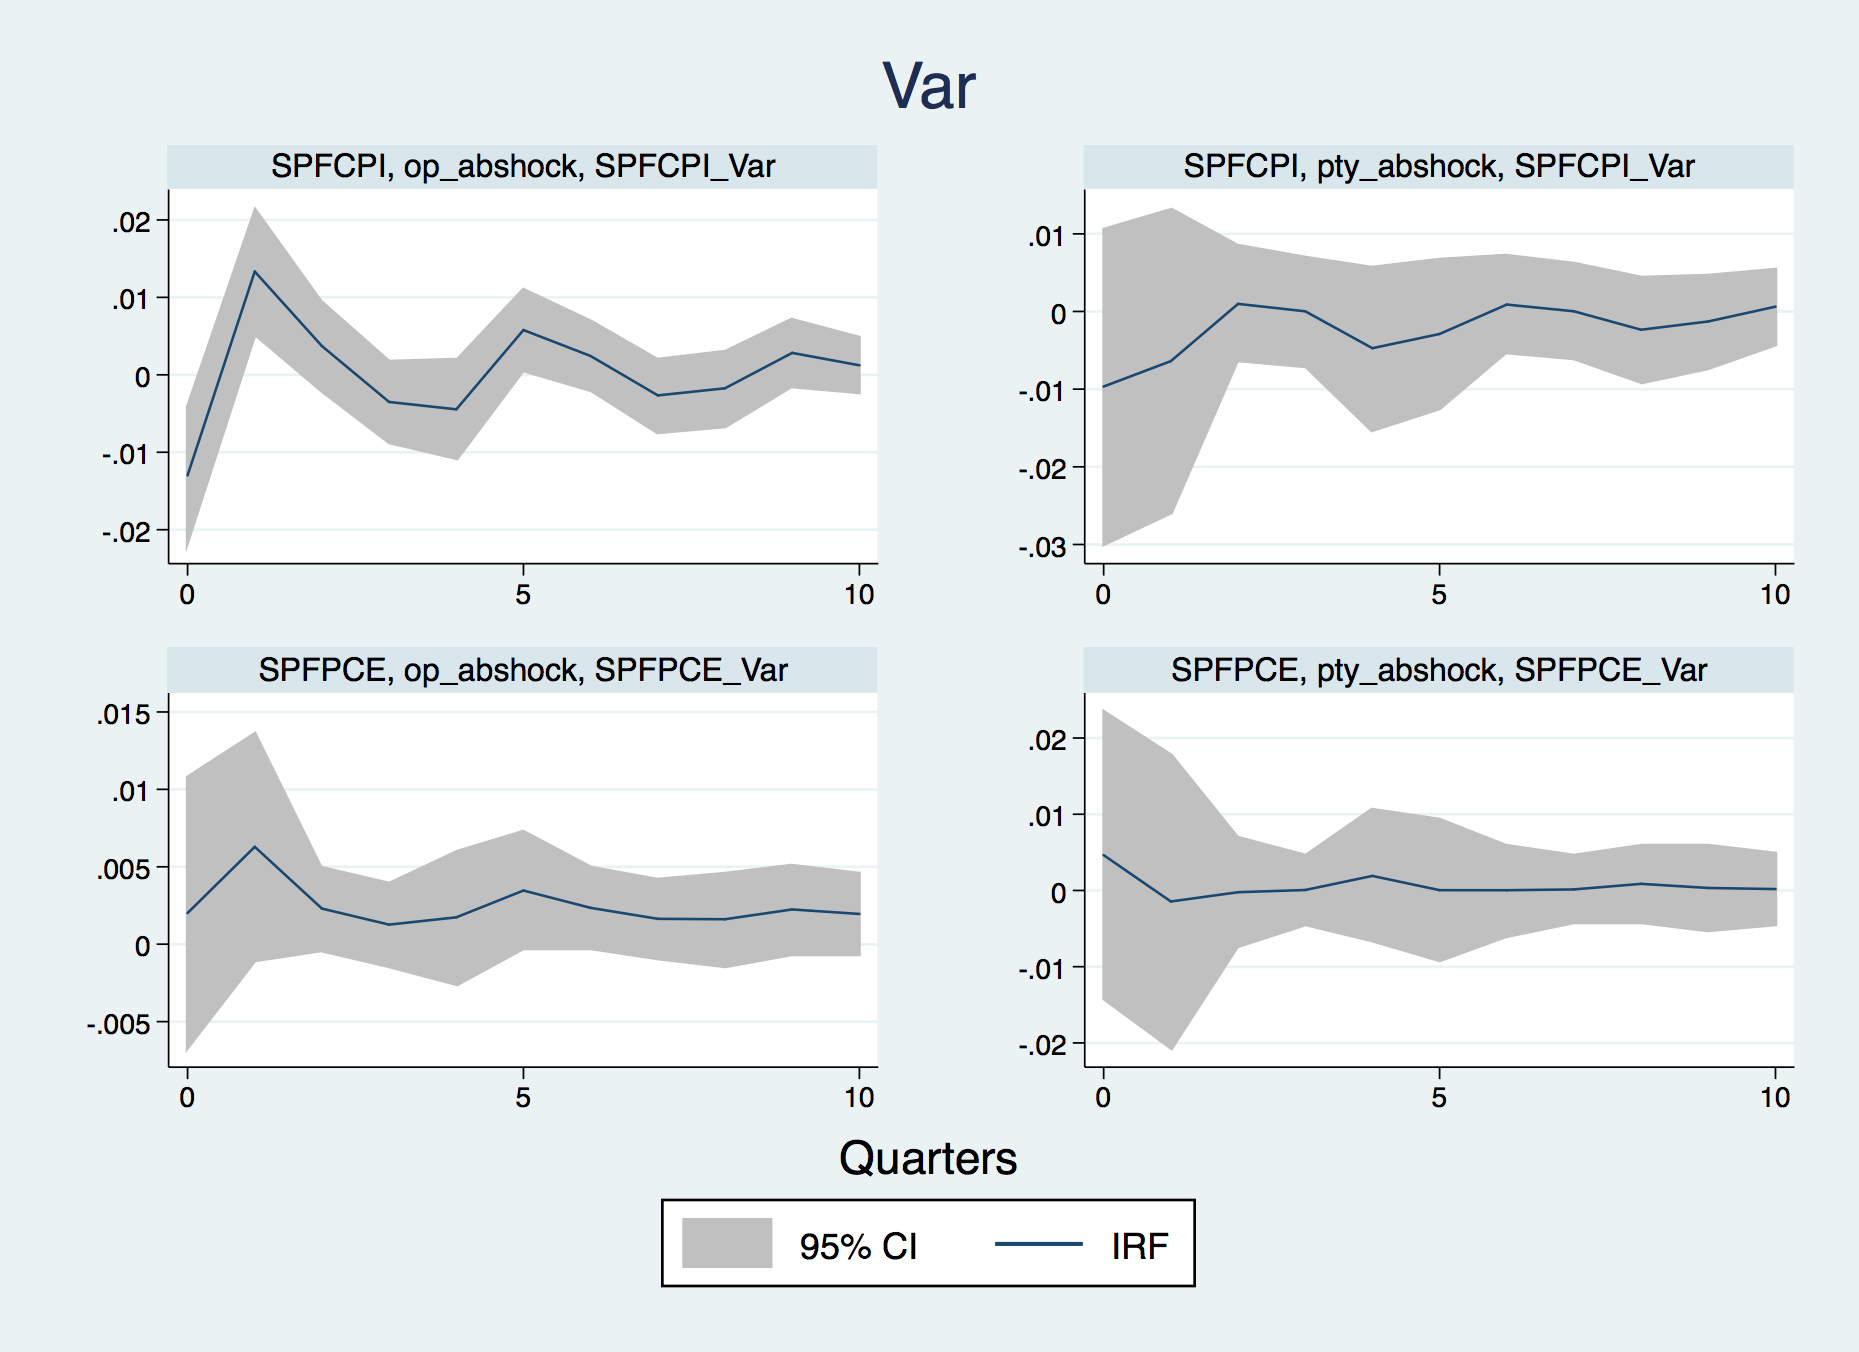
\includegraphics[width=7cm]{figuresDraft/SPFVar_ab_ashocks_nmp.png}  
\end{figure}

\end{frame}



\bibliographystyle{apalike}
\bibliography{ExpSlides}

\section{Appendix}




\begin{frame}{Sticky Expectation: individual}

For a non-updater since $t-\tau$ ($\tau=0$ for updater),
\begin{itemize}
\item \textbf{Mean} $$E_{i,t}(y_{t+h}|y_{t-\tau}) = \rho^{h+\tau} y_{t-\tau}$$  
\item \textbf{Forecast Error} $$FE_{i,t+h|t} = \underbrace{\sum^{h+\tau}_{s=0} \rho^s \omega_{t+h-s}}_{\substack{\text{weighted sum of} \\ \text{future realized shocks}} }$$
\item \textcolor{blue}{\textbf{Variance}} $$Var_{i,t}(y_{t+h}|y_{t-\tau}) = \sum^{h+\tau}_{s=0}\rho^{2s} \sigma^2_{\omega}$$	
\end{itemize}

\end{frame}


\begin{frame}{Sticky Expectation: individual}

$$\text{updater: } \quad \Delta Var_{i,t}(y_{t+h}|y_t)= \sum^{\tau}_{s=0} \rho^{2s}\sigma^2_{\omega}$$
$$\text{non-updater: }  \Delta Var_{i,t|t-\tau-1}(y_{t+h}|y_{t-\tau-1})  = \sigma^2_{\omega}$$


\begin{enumerate}
\item Change in expectation(and variance) depends on if update or not 
\item Cannot observe systematically sluggish response to shocks at individual level 
\end{enumerate}

\end{frame}



\begin{frame}{Sticky Expectation: population}
\begin{itemize}
	\item \textbf{Average forecast} 
	\begin{eqnarray*}
		\begin{aligned}
			\bar E_t(y_{t+h}) & = \lambda \underbrace{E_t(y_{t+h})}_{\text{rational expectation at t}} + (1-\lambda) \underbrace{\bar E_{t-1}(y_{t+h})}_{\text{average expectation at } t-1} \\
			& = \lambda E_t(y_{t+h}) + (1-\lambda) (\lambda E_{t-1}(y_{t+h})+ ...) \\
			& =\underbrace{ \lambda \sum^{\infty}_{s=0} (1-\lambda)^s E_{t-s}(y_{t+h})}_{\text{weighted sum of past rational expectations}}
		\end{aligned}
	\end{eqnarray*}
	\item \textbf{Change in average forecast}
	$$\Delta \bar E_t(y_{t+h})=\underbrace{(1-\lambda)}_{\text{stickiness}} \Delta \bar E_{t-1}(y_{t+h}) + \lambda \rho^h \omega_t$$ 
\end{itemize}
\end{frame}


\begin{frame}{Sticky Expectation: population}
\begin{itemize}
\item \textbf{Disagreements}
\begin{eqnarray*}
	\begin{aligned}
		Var_t(y_{t+h} ) & = \lambda \sum^{\infty}_{\tau=0} (1-\lambda)^{\tau} (E_{t|t-\tau}(y_{t+h}) - \bar E_t(y_{t+h}))^2  
	\end{aligned}
\end{eqnarray*}
\item \textbf{Change in disagreements}
$$\Delta Var_t (y_{t+h}) = \rho^{2h} (1-\lambda)\lambda \underbrace{\omega^2_t}_{\text{shock at time t}}$$
\end{itemize}

\begin{enumerate}
\item Disagreements rise after the shock and then gradually decline 
\item Response of disagreements depends on the size of the shock
\end{enumerate}
\end{frame}

\begin{frame}{Sticky Expectation: population}
\begin{itemize}
\item \textcolor{blue}{\textbf{Average variance}}
\begin{eqnarray*}
\begin{aligned}
	\overline {Var}_{t}(y_{t+h}) &  =  (1-\lambda)\underbrace{\overline {Var}_{t-1}(y_{t+h})}_{\text{average variance at t-1}} + \underbrace{\lambda Var_{t}(y_{t+h})}_{\text{variance of updater at t} }
\end{aligned}
\end{eqnarray*}
\item \textbf{Change in average variance}
$$\Delta \overline {Var}_{t}(y_{t+h}) = \underbrace{(1-\lambda)\Delta \overline {Var}_{t-1}(y_{t+h}) - \lambda \rho^{2h}\sigma^2_{\omega}}_{\text{does not depend on shock at t}}$$
\end{itemize}

\begin{enumerate}
\item Average variance does not respond to shocks
\item Average variance has serial correlation with the same rigidity parameter $1-\lambda$ 
\end{enumerate}

\end{frame}


\begin{frame}{Noisy Information: individuals}
\begin{itemize}
	\item \textbf{Mean}
	\begin{eqnarray*}
		\begin{aligned}
			E_{i,t}(y_{t+h}) & = \rho^{h}E_{i,t|t}(y_{t}) \\
			E_{i,t|t}(y_{t}) 
			& =  \underbrace{E_{i,t|t-1}(y_{t})}_{\text{prior}} + P \underbrace {(s_{i,t|t}-s_{i,t|t-1})}_{\text{innovations to signals}} \\
			& = (1-PH) E_{i,t|t-1}(y_{t}) + Ps_{i,t} \\
			\text{where }  & P = [P_\epsilon,P_\xi]= \Sigma^y_{i,t|t-1} H(H'\Sigma^y_{i,t|t-1} H + \Sigma^v)^{-1} \\
			\text {where } & \Sigma^y_{i,t|t-1} \text{ is the variance of } y_t \text{ based on prior belief}\\
			\text {and } & \Sigma^v =  \left[ \begin{matrix} 
				\sigma^2_{\epsilon} &  0 \\ 0 & \sigma^2_\xi \end{matrix}\right] 
		\end{aligned}
	\end{eqnarray*}
\end{itemize}
\end{frame}

\begin{frame}{Noisy Information: individuals}
\begin{itemize}
\item \textbf{Change in mean}
\begin{eqnarray*}
	\begin{aligned}
		\Delta E_{i,t|t}(y_{t+h}) & = \underbrace{\rho^h (1-PH)\Delta E_{i,t-1|t-1}(y_{t})}_{\text{Lagged response}} \\
		& + \underbrace{\rho^hPH \Delta y_{i,t} + \rho^h P\Delta v_{i,t}}_{\text{Shocks to signals}}\\
	\end{aligned}
\end{eqnarray*}
\end{itemize}

\begin{enumerate}
	\item Rigidity parameter $1-PH$
	\item Serial correlation at individual level 
	\item Always respond to shocks 
\end{enumerate}

\end{frame}

\begin{frame}{Noisy Information: individuals}
\begin{itemize}
	\item \textbf{Variance}
	
	\begin{eqnarray*}
		\begin{aligned}
			\Sigma^y_{i,t|t} = \Sigma^y_{i,t|t-1} - \Sigma^y_{i,t|t-1} H'(H \Sigma^y_{i,t-1} H' +\Sigma^v) ^{-1}H \Sigma^y_{i,t|t-1} 
		\end{aligned}
	\end{eqnarray*}
	\item \textbf{Change in variance} 
	$$\Delta \Sigma^y_{i,t|t} <0$$
	
\end{itemize}
\begin{enumerate}
	\item It does not depend on the realizations of the signal. 
	\item It decreases unambiguously from $t-1$ to $t$. 
	\item The two properties carry through to h-period ahead forecast 
\end{enumerate}

\end{frame}


\begin{frame}{Noisy Information: population}
\begin{itemize}
\item \textbf{Mean}

\begin{eqnarray*}
	\begin{aligned}
		\bar E_{t|t} (y_{t+h}) & = \rho^h [(1-PH) \underbrace{\bar E_{t-1}(y_{t+h})}_{\text{Average prior}} + P \underbrace{\bar s_{t}}_{\text{Average Signals}}] \\
		& = (1-PH) \bar E_{t-1}(y_{t+h}) + P [\epsilon_t, 0]' \\
		& = (1-PH) \bar E_{t-1}(y_{t+h}) + P \epsilon_t
	\end{aligned}
\end{eqnarray*}
\end{itemize}

\begin{enumerate}
	\item Same properties to the individual forecast 
\end{enumerate}

\end{frame}




\begin{frame}{Noisy Information: population}
\begin{itemize}
\item \textbf{Disagreements}
\begin{eqnarray*}
\begin{aligned}
	Var_t(y_{t+h}) & = E((E_{i,t|t}(y_{t+h}) - \bar E_t(y_{t+h}))^2) \\
	& = \rho^{2h} P^2_\xi \sigma^2_\xi  
\end{aligned}
\end{eqnarray*}
\end{itemize}

\begin{enumerate}
	\item increase with the forecast horizon
	\item depends on noisiness private signals, but not on that of public signals and the variance of the true variable $y$ 
	\item increase with the rigidity parameter $P$ in this model
\end{enumerate}

\end{frame}



\begin{frame}{Noisy Information: population}
\begin{itemize}
\item \textbf{Change in disagreements}
\begin{eqnarray*}
\begin{aligned}
\Delta Var_t(y_{t+h}) & = \rho^{2h}(1-\rho^2) P^2_\xi \sigma^2_\xi >0
\end{aligned}
\end{eqnarray*}
\end{itemize}

\begin{enumerate}
	\item disagreements increase as time goes from $t-1$ to $t$. 
	\item disagreements increase as approaching the variable of forecast
\end{enumerate}

\end{frame}


\begin{frame}{Noisy Information: population}
\begin{itemize}
\item \textbf{Average variance}
\begin{eqnarray*}
\begin{aligned}
\bar Var_t (y_{t+h}) = \bar \Sigma^y_t
\end{aligned}
\end{eqnarray*}
\item \textbf{Change in average variance}
\begin{eqnarray*}
\Delta Var_t(y_{t+h}) < 0 
\end{eqnarray*}

\end{itemize}

\begin{enumerate}
	\item average variance is the same as individual variance, not depend on signals
	\item the variance unambiguously drop over time 
\end{enumerate}

\end{frame}


\end{document}
